% NeurIPS 2026 anonymous-submission paper draft.
\documentclass{article}

% Official NeurIPS template hook for numeric citations.
\PassOptionsToPackage{numbers, compress}{natbib}

% Load NeurIPS style.
\usepackage{neurips_2026}

% Official template packages.
\usepackage[utf8]{inputenc}
\usepackage[T1]{fontenc}
\usepackage{hyperref}
\usepackage{url}
\usepackage{xcolor}
\usepackage{nicefrac}

% Packages (avoid loading natbib/geometry separately).
\usepackage{amsmath,amssymb,amsthm}
\usepackage{mathtools}
\usepackage{graphicx}
\usepackage{booktabs}
\usepackage{microtype}
\usepackage{enumitem}
\usepackage{subcaption}
\usepackage{changepage}
\usepackage{placeins}

% Algorithms
\usepackage{algorithm}
\usepackage{algorithmic}

% TikZ (load once)
\usepackage{tikz}
\usetikzlibrary{arrows.meta,calc,positioning}

\DeclareMathOperator*{\argmin}{arg\,min}
\DeclareMathOperator{\Var}{Var}

% Soft Bellman operator
\newcommand{\hatTs}{\widehat{\mathcal T}_{\mathrm{soft}}}
% Hard max Bellman operator
\newcommand{\Th}{\mathcal T_{\mathrm{hard}}}
\newcommand{\hard}{\mathrm{hard}}
\newcommand{\soft}{\mathrm{soft}}
\newcommand{\Cov}{\mathrm{Cov}}

\newcommand{\ALGCOMMENT}[1]{\item[]\texttt{\#~#1}}

\newcommand{\ProjF}{\Pi_{\mathcal F}}
\newcommand{\norm}[2][]{\left\| #2 \right\|_{#1}}
\newcommand{\inner}[3][]{\left\langle #2,\, #3 \right\rangle_{#1}}
\newcommand{\loc}{\mathrm{loc}}

\theoremstyle{plain}
\newtheorem{theorem}{Theorem}
\newtheorem{lemma}{Lemma}
\newtheorem{proposition}{Proposition}
\newtheorem{corollary}{Corollary}
\theoremstyle{definition}
\newtheorem{definition}{Definition}
\theoremstyle{remark}
\newtheorem{remark}{Remark}
\newtheorem{assumption}{Assumption}

\newcommand{\E}{\mathbb{E}}
% Optional short running title:

\title{Stationary Reweighting Yields Local Convergence of Soft Fitted Q-Iteration}

\author{%
  Lars van der Laan \\
  Department of Statistics, University of Washington \\
  \texttt{lvdlaan@uw.edu} \\
  \And
  Nathan Kallus \\
  Netflix and Cornell University
}

\begin{document}

\maketitle
\begin{abstract}
Fitted \(Q\)-iteration (FQI) and soft FQI are widely used value-based methods for
offline reinforcement learning, but their standard stability guarantees often
depend on Bellman completeness, a strong closure condition that can fail under
function approximation. We analyze soft FQI without Bellman completeness and
identify the stability mechanism that replaces it: local stationary norm
alignment. Near the soft-optimal fixed point, the soft Bellman operator has the
same first-order behavior as the policy-evaluation operator for the soft-optimal
policy. This operator contracts in the policy's stationary state-action norm,
whereas standard fitted regression projects Bellman targets in the behavior
norm. This mismatch explains instability under distribution shift. We use this
insight to develop stationary-reweighted soft FQI, which reweights each
regression step toward the stationary distribution of the current softmax policy.
Under approximate realizability and controlled weighting error, we prove
finite-sample local linear convergence to the projected fixed point, separating
statistical error from geometrically damped weight-estimation error. Our results
also show that ordinary soft FQI is locally stable under on-policy stationary
sampling, even without Bellman completeness, and explain temperature annealing as
a continuation strategy for reaching a contraction region.
\end{abstract}
\section{Introduction}

A core objective in reinforcement learning is to compute the optimal value
function, defined as the fixed point of a Bellman optimality equation
\citep{bellman1966dynamic}. The hard \(\max\) in this operator introduces
nondifferentiability and can exacerbate instability when combined with function
approximation and bootstrapping. Entropy regularization replaces the hard maximum
with a smooth softmax, yielding a differentiable Bellman operator that underlies
many modern value-based algorithms
\citep{ziebart2008maximum,ziebart2010causal,haarnoja2017reinforcement,
haarnoja2018soft}.
 


 



Fitted \(Q\)-iteration and its entropy-regularized analogue, \emph{soft} FQI,
approximate this fixed point by iterating projected Bellman updates: each step
forms bootstrapped one-step targets and regresses them onto a function class.
These methods are central in offline RL and large-scale approximate dynamic
programming
\citep{ernst2005tree,munos2005error,lazaric2012finite,uehara2023offline},
because they are simple to implement and compatible with off-the-shelf
supervised learners
\citep{voloshin2019empirical,fujimoto2019off,le2019batch,agarwal2021deep}.
When the function class is Bellman complete, standard analyses give
finite-sample guarantees for the projected Bellman iteration
\citep{gordon1995stable,tsitsiklis1996analysis,munos2008finite,
farahmand2010error,scherrer2014approximate,fan2020theoretical}.

However, fitted value-iteration methods can degrade under function approximation
and distribution shift when Bellman completeness fails
\citep{chen2019information,patterson2022generalized,vdLaanKallus2025FQE}. Information-theoretic,
hardness, and classical counterexample results show that, without additional
structure, offline value-function approximation can suffer poor horizon
dependence, exponential error amplification, or loss of convergence
\citep{chen2019information,foster2021offline,wang2021exponential,
amortila2020variant,meyn2024projected,gordon1995stable,baird1995residual,
tsitsiklis1996analysis}. These limitations have motivated minimax and adversarial \(Q\)-learning methods,
which relax Bellman completeness through saddle-point formulations
\citep{dai2018sbeed,uehara2020minimax,uehara2021finite,uehara2023offline,
jin2021bellman,xie2021batch}. However, they introduce more complex objectives,
auxiliary critic classes, and delicate optimization and tuning, moving away from
the simplicity of supervised learning.

In this paper, we revisit standard soft FQI and ask when it can remain stable
without Bellman completeness. We show that stability is governed by a local norm
mismatch. Near the soft-optimal solution, the projected soft Bellman update is
locally contractive in the stationary norm of the soft-optimal policy, whereas
standard soft FQI projects in the behavior-distribution norm. Under function approximation
and distribution shift, this mismatch can destroy local contraction. We therefore
propose stationary reweighting: a simple reweighting of the least-squares step
that targets the stabilizing stationary norm while retaining the supervised
learning structure of FQI\@.


\subsection{Contributions}

Our main contributions are:
\vspace{-0.25cm}
\begin{enumerate}[leftmargin=1.5em]

\item \textbf{Local contraction of projected soft value iteration.}
Near the soft-optimal solution, the soft Bellman operator has the same
first-order behavior as policy evaluation under the soft-optimal policy. This
identifies the policy's stationary distribution as the natural projection norm.
Under this projection, the fitted soft Bellman update is locally contractive and
converges linearly, even without Bellman completeness.

\item \textbf{Stationary reweighting for off-policy data.}
We approximate the stationary-norm projection from behavior data by reweighting
each Bellman regression with estimated stationary state-action density ratios.
Exact ratios are unnecessary; the weights only need to preserve the stabilizing
projection norm up to controlled error.

\item \textbf{Finite-sample local convergence guarantees without Bellman completeness.}
We prove finite-sample local convergence for stationary-reweighted soft FQI\@.
Inside a contraction basin, the iterates converge linearly up to statistical and
weight-estimation errors, with weight errors damped geometrically across
iterations. As a special case, ordinary unweighted soft FQI is locally stable under
on-policy stationary sampling, even without Bellman completeness.

\end{enumerate}
\vspace{-0.25cm}

\textbf{Scope.}
Our guarantees are local: they show that stationary reweighting stabilizes soft
FQI within a contraction basin of the population projected update. We do not
prove basin entry from arbitrary offline initializations, and we condition on
sufficiently accurate stationary-ratio weights. Section~\ref{sec::algo} and
Appendix~\ref{app:homotopy} discuss warm starts and temperature annealing as one possible
basin-entry strategy; Appendix~\ref{app:ratio-estimation} discusses estimation of stationary ratios using DICE-style, minimax, and emphatic occupancy-ratio methods
\citep{liu2018breaking,nachum2019dualdice,zhang2020gendice,
uehara2020minimax,sutton2016emphatic,hallak2016generalized}.

\subsection{Related Work}

Several approaches address instability of fitted Bellman updates under function
approximation and distribution shift. One line strengthens the approximation
structure through linear or low-rank assumptions, representation learning, or
state-space discretization
\citep{melo2007convergence,duan2020minimax,yang2020reinforcement,
jin2023provably,chang2022learning,peng1993convergence,van2006performance,
xie2021batch}. Classical FQE/FQI analyses typically handle distribution shift through
concentrability or distribution-mismatch constants
\citep{munos2008finite,scherrer2014approximate,fan2020theoretical,
xie2022role}. Another line replaces least-squares Bellman regression with
minimax, adversarial, or pessimistic Bellman-error objectives
\citep{uehara2020minimax,jin2021bellman,xie2021batch,uehara2023offline,
xie2021bellman}. These methods test Bellman residuals against auxiliary critic
classes and obtain guarantees under conditions such as partial coverage, dual
realizability, or critic richness. Related entropy-regularized control methods
\citep{ziebart2008maximum,haarnoja2018soft,geist2019theory,neu2017unified,
zhan2023policy,lan2023policy}
optimize policies directly rather than through regression-based fixed-point
iteration. In contrast, we keep the fitted soft \(Q\)-iteration template and ask
whether changing only the regression norm can restore local contraction.

Weighting methods play several related roles in reinforcement learning.
Importance sampling reweights returns or trajectories for off-policy evaluation
\citep{precup2000eligibility,precup2001off,thomas2016data,de2023value}, while
density-ratio and DICE-style methods estimate stationary or discounted occupancy
corrections for off-policy evaluation and learning
\citep{liu2018breaking,hallak2017consistent,nachum2019dualdice,
zhang2020gendice,uehara2020minimax}. Emphatic weighting is closest in
motivation: it reweights Bellman-style TD recursions to mitigate off-policy
bootstrapping instability, mainly in policy evaluation
\citep{yu2012weighted,mahmood2015emphatic,sutton2016emphatic,
hallak2016generalized,yu2018generalized,patterson2022generalized}.
Stable ratio estimation under nonlinear approximation and limited coverage
remains difficult, motivating regularization, variance control, and truncation
\citep{zhang2022truncated,mehrabi2024off,uehara2021finite}.

Our setting differs from this literature in two ways. First, we study fitted
soft \(Q\)-iteration, where weights define the projection norm in a
least-squares Bellman regression rather than update weights in a TD recursion.
Second, the relevant ratio is induced by the optimal policy and is therefore
coupled to the Bellman fixed point. For policy evaluation, prior work has shown
that stationary ratios can stabilize Bellman-based methods, including TD
learning and FQE
\citep{van2006performance,patterson2022generalized,vdLaanKallus2025FQE}. We
show that, in soft control, the optimal stationary ratio defines the local
projection norm for soft FQI, yielding local contraction near the
soft-optimal fixed point without Bellman completeness or global contraction of
the projected operator.  

\section{Preliminaries}
\label{sec:preliminaries}

\subsection{Soft Optimal Control}
\label{subsec:soft-optimal-control}

We consider a discounted MDP with continuous state space \(\mathcal S\), finite action
space \(\mathcal A\), transition kernel \(P\), reward \(r_0\), discount
\(\gamma\in[0,1)\), and behavior distribution \(\nu_b\) over
\(\mathcal S\times\mathcal A\). For any \(Q:\mathcal S\times\mathcal A\to
\mathbb R\) and temperature \(\tau>0\), define the softmax policy
\[
\pi_Q(a\mid s)
=
\frac{\exp\{Q(s,a)/\tau\}}
     {\sum_{b\in\mathcal A}\exp\{Q(s,b)/\tau\}}.
\]

The \textbf{soft Bellman optimality operator} \citep{haarnoja2017reinforcement,haarnoja2018soft,uehara2023offline} is
\[
(\mathcal T Q)(s,a)
=
r_0(s,a)
+\gamma\,\E_{S'\sim P(\cdot\mid s,a)}
\left[
\tau \log \sum_{a'\in\mathcal A} e^{Q(S',a')/\tau}
\right].
\]
The \textbf{soft optimal \(Q\)-function} \(Q^\star\) is the unique bounded fixed
point of \(\mathcal T\), equivalently the \(Q\)-function maximizing the
entropy-regularized discounted return. The \textbf{soft optimal
policy} is \(\pi^\star:=\pi_{Q^\star}\).

Our local analysis uses the policy-evaluation operator obtained by freezing the
softmax policy at \(Q\). Let \(\mathsf H(\pi_Q(\cdot\mid S'))\) denote the
Shannon entropy of \(\pi_Q\) at \(S'\), and define
\[
\tilde r_Q(s,a)
:=
r_0(s,a)
+
\gamma\,\E_{S'\sim P(\cdot\mid s,a)}
\bigl[\tau\,\mathsf H(\pi_Q(\cdot\mid S'))\bigr],
\]
\[
\begin{aligned}
\mathcal T^{\mathrm{eval}}_{Q}f(s,a)
&:=
\tilde r_Q(s,a)
+
\gamma(P^{\mathrm{eval}}_{\pi_Q}f)(s,a),\\
(P^{\mathrm{eval}}_{\pi_Q}f)(s,a)
&:=
\E_{S'\sim P(\cdot\mid s,a),\,A'\sim\pi_Q(\cdot\mid S')}
\bigl[f(S',A')\bigr].
\end{aligned}
\]
The
entropy-regularized \textbf{Bellman evaluation operator} for the soft-optimal policy is \(\mathcal{T}^{\mathrm{eval}}_{Q^\star}\) .

Let \(\mu^\star:=\mu_{\pi^\star}\) denote the \textbf{stationary state--action
distribution} induced by \((P,\pi^\star)\). Let \(L^2(\mu^\star)\) be the Hilbert space
of functions \(f:\mathcal S\times\mathcal A\to\mathbb R\) satisfying
\(\E_{\mu^\star}[f(S,A)^2]<\infty\), equipped with norm
\[
\|f\|_{2,\mu^\star}
:=
\bigl(\E_{\mu^\star}[f(S,A)^2]\bigr)^{1/2}.
\]
Under the stationary norm, \(\mathcal T^{\mathrm{eval}}_{Q^\star}\) is a
\(\gamma\)-contraction
\citep{bertsekas1996neuro,hallak2016generalized,patterson2022generalized,
vdLaanKallus2025FQE}. For any nonnegative weight \(d\), write \(d\cdot\nu_b\)
for the distribution with \(\nu_b\)-density \(d\); in particular,
\((d\mu^\star/d\nu_b)\cdot\nu_b=\mu^\star\).

\subsection{Stationary reweighting: intuition and population target}
\label{sec:prelim-fqi-weighting}

The standard convergence argument for soft value iteration relies on the soft
Bellman operator \(\mathcal T\) being a \(\gamma\)-contraction in the sup norm:
iterating \(\mathcal T\) from any bounded initialization converges to its unique
fixed point
\citep{bellman1966dynamic,puterman1990markov,bertsekas1996neuro,
geist2019theory}. With function approximation, fitted \(Q\)-iteration does not
iterate \(\mathcal T\) directly. Instead, each Bellman update is projected back
onto the function class \(\mathcal F\), typically by least squares in the
behavior norm \(L^2(\nu_b)\) \citep{munos2008finite}. If \(\mathcal F\) is
Bellman complete, so that \(\mathcal T(\mathcal F)\subseteq\mathcal F\), this
projection is harmless. Without completeness, however, FQI iterates the
projected operator \(\Pi_{\nu_b}\mathcal T\). The difficulty is that
\(\Pi_{\nu_b}\) is nonexpansive only in \(L^2(\nu_b)\), not in the sup norm.
Thus \(\Pi_{\nu_b}\mathcal T\) need not inherit the \(\gamma\)-contraction of
\(\mathcal T\): projection can distort Bellman errors rather than contract them,
breaking the stability argument for exact value iteration
\citep{gordon1995stable,tsitsiklis1996analysis,chen2019information}.

The issue is not projection itself, but projection in a norm misaligned with
the local Bellman dynamics. Near the soft-optimal fixed point \(Q^\star\), the
soft Bellman operator is first-order equivalent to policy evaluation under the
soft-optimal policy \(\pi^\star\):
\begin{equation}
\label{eqn::linapprox}
\mathcal T(Q)
\;\approx\;
Q^\star + \gamma\,P^{\mathrm{eval}}_{\pi^\star}(Q - Q^\star)
\;=\;
\mathcal{T}^{\mathrm{eval}}_{Q^\star}(Q).
\end{equation}
This follows from the Fréchet derivative identity
\(D\mathcal T(Q)[H]=\gamma P^{\mathrm{eval}}_{\pi_Q}H\), stated formally in
Lemma~\ref{lem:first-derivative}. Since \(P^{\mathrm{eval}}_{\pi^\star}\) is
nonexpansive in \(L^2(\mu^\star)\), the linearized update is a
\(\gamma\)-contraction in the stationary norm
\citep{patterson2022generalized,vdLaanKallus2025FQE}. Thus, the natural local
projection norm is \(L^2(\mu^\star)\), not the behavior norm \(L^2(\nu_b)\).

This motivates replacing the behavior-norm projection with a stationary-norm
projection. Assume \(\mu^\star\ll\nu_b\), and let
\(d^\star:=d\mu^\star/d\nu_b\). The population stationary-weighted update is
\begin{equation}
Q^{(k+1)}
=
\argmin_{f\in\mathcal F}
E_{\nu_b}\!\left[
d^\star(S,A)\{\mathcal T(Q^{(k)})(S,A)-f(S,A)\}^2
\right]
=
\Pi_{\mathcal F}\mathcal T(Q^{(k)}),
\label{eqn::fixedpointmap}
\end{equation}
where \(\Pi_{\mathcal F}\) is the \(L^2(\mu^\star)\)-projection onto
\(\mathcal F\).  Since this projection is nonexpansive in the norm where the
linearized Bellman update contracts, the projected operator can inherit local
contraction. We make this precise in Section \ref{sec:local-geometry}. 

The ideal update \eqref{eqn::fixedpointmap} is not directly implementable,
because \(\mu^\star\) depends on the unknown optimal policy. Instead, it defines
the population norm that the fitted regression should approximate. Section
\ref{sec:stationary-reweighted-fqi} implements this idea by estimating Bellman
targets from behavior data and weighting observations by density ratios for the
stationary distribution of the current softmax policy \(\pi_{Q^{(k)}}\). Near
\(Q^\star\), the stationary distribution of \(\pi_{Q^{(k)}}\) is close to
\(\mu^\star\), so iterative reweighting approximates the ideal stationary
projection. Section~\ref{sec::finitesample} gives finite-sample theory.

\section{Local Contraction and Convergence of Soft \(Q\)-Iteration}
\label{sec:local-geometry}
\subsection{Local approximation and contraction}
 

We first control the linearization remainder in \eqref{eqn::linapprox} through a
local smoothness condition around \(Q^\star\). This shows that, near
\(Q^\star\), the projected soft Bellman operator \(\mathcal T_{\mathcal F}\) is
a locally contractive perturbation of the policy-evaluation operator
\(\mathcal T^{\mathrm{eval}}_{Q^\star}\).

For \(r>0\) and \(Q_0\in L^2(\mu^\star)\), write
\[
\mathbb B_{\mathcal F}(r,Q_0)
:=
\{f\in\mathcal F:\|f-Q_0\|_{2,\mu^\star}\le r\},
\qquad
\mathcal H_{\mathcal F}^\star
:=
\{Q_1-Q_2:Q_1,Q_2\in\mathcal F\cup\{Q^\star\}\}.
\]
For \(R>0\), define the \(Q^\star\)-star hull of the local model ball
\[
\mathbb S_{\mathcal F}^\star(R)
:=
\{Q^\star+t(f-Q^\star):f\in\mathbb B_{\mathcal F}(R,Q^\star),\ t\in[0,1]\},
\]
and define the local Bellman derivative modulus
\[
\omega_{\mathcal T}(R)
:=
\sup_{\substack{
Q\in\mathbb S_{\mathcal F}^\star(R)\\
H\in\mathcal H_{\mathcal F}^\star,\ H\ne0}}
\frac{
\|(D\mathcal T(Q)-D\mathcal T(Q^\star))[H]\|_{2,\mu^\star}
}{
\|H\|_{2,\mu^\star}
}.
\]

\begin{enumerate}[label=\textbf{C\arabic*)}, ref={C\arabic*}, leftmargin=1.5em, series=cond]
\item \label{cond::posit}
\textbf{Stationary action positivity.}
Exists \(\pi_{\min}>0\) such that
\(\pi^\star(A\mid S)\ge \pi_{\min}\) \(\mu^\star\)-almost surely.

\item \label{cond::convex}
\textbf{Model class regularity.}
\(\mathcal F\subseteq L^2(\mu^\star)\) is convex, closed, and uniformly bounded.

\item \label{cond::curvature}
\textbf{Local Bellman curvature.}
\(\omega_{\mathcal T}(R)\to0\) as \(R\downarrow0\).
\end{enumerate}

Condition~\ref{cond::posit} gives stationary action positivity, and
Condition~\ref{cond::convex} is standard for convex linear-model constraints,
such as \(\ell^1\)- and \(\ell^2\)-balls. Condition~\ref{cond::curvature} is the
only local smoothness requirement: it asks that the derivative of the soft
Bellman operator be continuous, in stationary norm, along directions relevant to
the local projected iteration. Appendices \ref{app:proof-curvature-calibrations} and \ref{app:c3-examples} give sufficient conditions under
which \(\omega_{\mathcal T}(R)\lesssim R^\alpha\) for some
\(\alpha\in(0,1]\), using \(L^\infty\)--\(L^2\) interpolation for
finite-dimensional, H\"older, Sobolev, and RKHS classes.
Appendix~\ref{app:tausmall} shows that, under action-gap conditions, the
hard-max limit can also be handled: the local curvature modulus remains small on
shrinking neighborhoods as \(\tau\downarrow0\).

Define the local contraction modulus and radius by
\[
\rho_{\mathrm{loc}}(R):=\gamma+\omega_{\mathcal T}(R),
\qquad
r_{\mathrm{loc}}:=\sup\{R>0:\rho_{\mathrm{loc}}(R)<1\}.
\]


\begin{lemma}[Linearization remainder]
\label{lem:second-order-remainder}
Under Conditions~\ref{cond::posit}--\ref{cond::curvature}, for any
\(R<r_{\mathrm{loc}}\) and any
\(Q \in \mathbb B_{\mathcal F}(R,Q^\star)\),
\[
\bigl\|\mathcal{T}(Q)-\mathcal{T}^{\mathrm{eval}}_{Q^\star}(Q)\bigr\|_{2,\mu^\star}
\;\le\;
\omega_{\mathcal T}(R)\,\|Q-Q^\star\|_{2,\mu^\star}.
\]
\end{lemma}

Combining the preceding lemma with the global \(\gamma\)-contraction of
\(\mathcal T^{\mathrm{eval}}_{Q^\star}\) in \(L^2(\mu^\star)\) gives a local
contraction bound for \(\mathcal T_{\mathcal F}\). By definition of
\(r_{\mathrm{loc}}\), the linearization error is smaller than the contraction
margin on every ball of radius \(R<r_{\mathrm{loc}}\). Hence the contraction
argument applies on
\(\mathbb B_{\mathcal F}(r_{\mathrm{loc}},Q^\star)\), provided this set is
nonempty, namely when
\[
\mathrm{dist}(\mathcal F,Q^\star)
:=
\|\Pi_{\mathcal F}Q^\star-Q^\star\|_{2,\mu^\star}
\le r_{\mathrm{loc}} .
\]

\begin{theorem}[Local contraction of the projected soft Bellman operator]
\label{thm:local-contraction}
Assume Conditions~\ref{cond::posit}--\ref{cond::curvature} hold. For any
\(R \in [\mathrm{dist}(\mathcal F,Q^\star),\, r_{\mathrm{loc}})\),
\(\mathcal{T}_{\mathcal F} = \Pi_{\mathcal F} \mathcal T\)
is a \(\rho_{\mathrm{loc}}(R)\)-contraction on
\(\mathbb{B}_{\mathcal{F}}(R,Q^\star)\): for all
\(Q_1,Q_2 \in \mathbb{B}_{\mathcal{F}}(R,Q^\star)\),
\[
\|\mathcal{T}_{\mathcal F}(Q_1)
- \mathcal{T}_{\mathcal F}(Q_2)\|_{2,\mu^\star}
\;\le\;
\rho_{\mathrm{loc}}(R)\,\|Q_1 - Q_2\|_{2,\mu^\star}.
\]
\end{theorem}
 

\subsection{Local convergence of soft \(Q\)-iteration}

If the approximation error is small relative to the local contraction margin,
Banach's fixed-point theorem gives a unique projected fixed point near
\(Q^\star\). We impose the following condition.

\begin{enumerate}[label=\textbf{C\arabic*)}, ref={C\arabic*}, leftmargin=1.5em, resume=cond]
\item \label{cond::eps-small}
\textbf{Approximate realizability.}
There exists \(R_{\mathrm{fp}}\in(0,r_{\mathrm{loc}})\) such that
\[
\mathrm{dist}(\mathcal F,Q^\star)
\le
\{1-\rho_{\mathrm{loc}}(R_{\mathrm{fp}})\}R_{\mathrm{fp}}.
\]
\end{enumerate}

By Lemma~\ref{lem:proj-fixed-point}, Condition~\ref{cond::eps-small} ensures
that \(\mathcal T_{\mathcal F}\) has a fixed point \(Q^\dagger\in\mathcal F\)
inside the local contraction region:
\[
Q^\dagger=\mathcal T_{\mathcal F}(Q^\dagger),
\qquad
\varepsilon_{\mathcal F}
:=
\|Q^\dagger-Q^\star\|_{2,\mu^\star}.
\]
We next show that soft \(Q\)-iteration converges linearly when initialized near
\(Q^\dagger\). Since the contraction region is centered at \(Q^\star\), any ball
\(\mathbb B_{\mathcal F}(r,Q^\dagger)\) with
\(r+\varepsilon_{\mathcal F}<r_{\mathrm{loc}}\) is contained in the local
contraction region around \(Q^\star\).

\begin{theorem}[Local linear convergence around the projected soft optimum]
\label{thm:local-linear}
Assume Conditions~\ref{cond::posit}--\ref{cond::eps-small} hold. Let
\(r>0\) satisfy $r+\varepsilon_{\mathcal F}<r_{\mathrm{loc}}.$ 
Then, for any initialization
\(Q^{(0)}\in\mathbb B_{\mathcal F}(r,Q^\dagger)\) and all \(k\ge0\),
\[
\|Q^{(k)} - Q^\dagger\|_{2,\mu^\star}
\le
\{\rho_{\mathrm{loc}}(r+\varepsilon_{\mathcal F})\}^k
\|Q^{(0)} - Q^\dagger\|_{2,\mu^\star}.
\]
\end{theorem}

The theorem shows that soft \(Q\)-iteration is locally contractive around
\(Q^\dagger\): within any admissible ball
\(\mathbb B_{\mathcal F}(r,Q^\dagger)\) with
\(r+\varepsilon_{\mathcal F}<r_{\mathrm{loc}}\), the
iterates move toward \(Q^\dagger\) at rate
\(\rho_{\mathrm{loc}}(r+\varepsilon_{\mathcal F})\). As the iterates approach \(Q^\dagger\),
they enter smaller basins with sharper contraction moduli. In the realizable
case, the modulus approaches \(\gamma\) at a geometric rate; see
Corollary~\ref{cor:finite-time-tightening} in Appendix~\ref{app:rate-tightening}.

\section{Stationary-Reweighted Soft FQI}
\label{sec:stationary-reweighted-fqi}
\label{sec::algo}

The preceding section identifies the ideal stationary-norm update
\(\mathcal T_{\mathcal F}=\Pi_{\mathcal F}\mathcal T\). Stationary-reweighted
soft FQI approximates this update from behavior data by weighting each Bellman
regression with an estimated stationary density ratio. This section gives the
finite-sample algorithm.

\textbf{Algorithm.}
Given offline transitions
\(\mathcal D_n := \{(S_i,A_i,R_i,S_i')\}_{i=1}^n\) sampled from \(\nu_b\) and a
function class \(\mathcal F\), initialize \(\widehat Q^{(0)}\). For the induced
policy \(\pi_{\widehat Q^{(0)}}\), estimate weights \(\widehat d^{(0)}\)
targeting the stationary ratio
\(\mathrm d\mu_{\pi_{\widehat Q^{(0)}}}/\mathrm d\nu_b\).

For each \(k \in \{0,\dots,K-1\}\), form the empirical soft Bellman targets
\[
\widehat y_i^{(k)}
=
R_i
+
\gamma\tau \log \sum_{a'}
\exp\!\bigl(\widehat Q^{(k)}(S_i',a')/\tau\bigr).
\]
Then update the \(Q\)-estimate by weighted least squares:
\[
\widehat Q^{(k+1)}
\in
\argmin_{Q\in\mathcal F}
\frac{1}{n}\sum_{i=1}^n
\widehat d^{(k)}(S_i,A_i)\,
\bigl(\widehat y_i^{(k)}-Q(S_i,A_i)\bigr)^2.
\]
Finally, estimate weights \(\widehat d^{(k+1)}\) for the updated policy
\(\pi_{\widehat Q^{(k+1)}}\) and continue. 


\textbf{Computation.} Each iteration adds a density-ratio estimation step to the usual
Bellman regression step. In practice, neither the \(Q\)-function nor the density
ratio must be solved to completion at every iteration. One can instead
parametrize both \(Q\) and \(d\) with neural networks and alternate between one or
a few stochastic-gradient updates for each, as in deep fitted \(Q\)-learning or
boosting-style fitted value iteration
\citep{riedmiller2005neural,tosatto2017boosted}.

\textbf{Estimating stationary ratios.}
The stationary state-action density ratio can be estimated using existing
off-policy evaluation tools, including DICE-style saddle-point methods
\citep{liu2018breaking,nachum2019dualdice,nachum2019algaedice,
zhang2020gendice,lee2021optidice,lee2022coptidice}, minimax weight estimators
\citep{uehara2020minimax,uehara2021finite}, and projected or balancing-weight
methods \citep{wang2023projected}; see Appendix~\ref{app:ratio-estimation}.
With linear or RKHS critics, these objectives often reduce to tractable
linear-system or closed-form updates
\citep{dikkala2020minimax,uehara2020minimax,wang2023projected,
olivas2025source}. Existing finite-sample guarantees apply under conditions such
as realizability, completeness, coverage, and identification
\citep{uehara2021finite}. Stationary ratios are the undiscounted analogues of
discounted occupancy ratios, which are central to importance-sampling, doubly
robust, and efficient policy-value estimators
\citep{jiang2016doubly,thomas2016data,kallus2020double,kallus2022efficiently,
amortila2024harnessing}. In our setting, the ratio plays a different role: it
stabilizes the Bellman regression geometry rather than only debiasing a final
policy-value estimate.

\textbf{Initialization, warm starts, and temperature annealing.}
Our guarantees are local: they apply once the iterates lie in a basin where the
stationary projected Bellman update is contractive. Standard soft FQI can be
used as a warm start for reaching this basin. For example, under approximate
Bellman completeness, standard soft FQI may approach \(Q^\dagger\) up to an
inherent Bellman error \citep{munos2008finite}; if this error is smaller than
the contraction radius, the local guarantee applies from that point onward.
After the switch to stationary weighting, the recursion contracts toward the
stationary projected fixed point, and the finite-sample bound no longer
accumulates the classical inherent Bellman-error term.

Temperature annealing provides another basin-entry heuristic, inspired by
classical continuation and deterministic annealing methods
\citep{allgower1990numerical,rose2002deterministic}. At large temperature
\(\tau\), the soft Bellman update is smoother, the local contraction basin can
be larger, and the optimal soft policy is closer to uniform. Thus, one can start
from a simple initialization, approximate the initial stationary ratio by that
of the uniform policy, and then gradually decrease \(\tau\), warm-starting each
stage from the previous solution while updating the stationary-ratio estimate.
If consecutive basins overlap, the iterates remain locally stable along the
annealing path. Appendix~\ref{app:homotopy} gives a population-level
continuation argument and shows that, under an action-gap condition, this path
can approach the hard-max limit. A full finite-sample analysis of the annealing
scheme is left for future work.

\section{Finite-Sample Convergence Analysis}
\label{sec::finitesample}

We prove the finite-sample guarantee for stationary-reweighted soft FQI\@.
Theorem~\ref{thm:convergencemain} shows that, within an admissible local basin,
the iterates contract toward \(Q^\dagger\) up to statistical error from empirical
Bellman regression and geometrically damped weight-estimation error. The proof
combines: (i) an inexact local Picard recursion, (ii) a high-probability bound
for one weighted Bellman regression, and (iii) a localization argument that keeps
the iterates inside the contraction basin.

\subsection{Inexact local Picard iteration}

We first establish a local analogue of the classical FQI recursion of
\citet{munos2008finite}. Since contraction holds only inside a local basin, the
per-iteration errors need not be zero, but must be small relative to the
contraction margin.

\begin{lemma}[Local inexact iteration error bound]
\label{lem:inexact-fqi}
Assume Conditions~\ref{cond::posit}--\ref{cond::eps-small}. Fix
\(r>0\) satisfying \(r+\varepsilon_{\mathcal F}<r_{\mathrm{loc}}\), and set
\(\rho_r:=\rho_{\mathrm{loc}}(r+\varepsilon_{\mathcal F})\). Suppose that, for some nonnegative
sequence \(\{\xi_k\}_{k\ge0}\), the inexact iterates satisfy
\[
\|\mathcal T_{\mathcal F}(\widehat Q^{(k)}) - \widehat Q^{(k+1)}\|_{2,\mu^\star}\le \xi_k,\quad
\|\widehat Q^{(0)}-Q^\dagger\|_{2,\mu^\star}\le r,\quad
\xi_k\le (1-\rho_r)r.
\]
Then, for every \(k\ge0\),
\[
\|\widehat Q^{(k)}-Q^\dagger\|_{2,\mu^\star}
\le
\rho_r^k\|\widehat Q^{(0)}-Q^\dagger\|_{2,\mu^\star}
+
\sum_{j=0}^{k-1}\rho_r^{k-1-j}\xi_j.
\]
\end{lemma}

The condition \(\xi_k \le (1-\rho_r)r\) is the local-basin slack condition:
at the boundary of the basin, contraction pulls the iterate inward by
\((1-\rho_r)r\), and the one-step error must fit within this margin.
Under this condition, Lemma~\ref{lem:inexact-fqi} yields linear convergence up
to the inexactness floor
\(\sum_{j=0}^{k-1} \rho_r^{\,k-1-j}\xi_j\).

\subsection{Finite-sample bounds on the per-iteration error}

We next bound the per-iteration inexactness $\|\mathcal T_{\mathcal F}(\widehat Q^{(k)})
  -\widehat Q^{(k+1)}\|_{2,\mu^\star}$ with high probability, separating sampling noise, approximation error, and
weight-estimation error. We express the ERM rates through metric entropy. Let
\(N(\varepsilon,\mathcal F,L^2(P))\) denote the \(L^2(P)\)-covering number, and
define
\[
\mathcal J(\delta,\mathcal F)
:=
\int_0^\delta
\sup_P
\sqrt{\log N(\varepsilon,\mathcal F,L^2(P))}\,d\varepsilon,
\qquad
\delta_n
:=
\inf\left\{
\delta>0:
\mathcal J(\delta,\mathcal F)
\le
\sqrt n\,\delta^2
\right\}.
\]
Then \(\delta_n\) yields the standard ERM rates over \(\mathcal F\)
\citep{wainwright2019high}; for example,
\(\delta_n\asymp \sqrt{s\log(d/s)/n}\) for \(s\)-sparse linear models,
\(\delta_n\asymp \sqrt{V\log(n/V)/n}\) for VC-subgraph classes, and
\(\delta_n\asymp n^{-s/(2s+d)}\) for H\"older/Sobolev classes of smoothness
\(s\) in dimension \(d\le 2s\) \citep{wainwright2019high}.

\begin{enumerate}[label=\textbf{C\arabic*)}, ref={C\arabic*}, leftmargin=1.5em, resume=cond]
\item \label{cond::bounded}
\textbf{Bounded regression objects.}
There exists \(M<\infty\) such that \(|R|\le M\) and
\(\sup_{f\in\mathcal F}\|f\|_\infty\le M\).

\item \label{cond::weight-coverage}
\textbf{Coverage and bounded weights.}
\(\mu^\star\ll\nu_b\) and there exists
\(1\le\kappa_{\mathrm{cov}}<\infty\) such that, for all \(0\le k\le K-1\),
\[
\|d^\star\|_\infty\le \kappa_{\mathrm{cov}},
\qquad
\|\widehat d^{(k)}\|_\infty\le \kappa_{\mathrm{cov}},
\qquad
\|(\widehat d^{(k)}-d^\star)/\sqrt{d^\star}\|_\infty
\le \kappa_{\mathrm{cov}} .
\]

\item \label{cond::split}
\textbf{Sample splitting.}
The weight estimators \(\{\widehat d^{(k)}\}_{k=0}^K\) are computed
using data independent of the batch \(\mathcal{D}_n\) used for the regression
updates.

\item \label{cond::entropy}
\textbf{Entropy integral regularity.}
 \(\mathcal J(\infty, \mathcal F) < \infty\),
\(\mathcal J(\delta,\mathcal F)/
\{\delta \sqrt{\log\!\log(1/\delta)}\}\to\infty\) as \(\delta\to 0\).
\end{enumerate}
Condition~\ref{cond::bounded} simplifies the analysis and can be relaxed using
truncation and tail conditions \citep{wainwright2019high}.
Condition~\ref{cond::weight-coverage} imposes bounded target--behavior coverage
and keeps the estimated weights controlled. It is the analogue of coverage or
concentrability assumptions in offline RL
\citep{xie2022role,uehara2020minimax}.
Condition~\ref{cond::split} ensures independence between weight estimation and
the regression sample and can be removed by cross-fitting
\citep{nie2021quasi,foster2023orthogonal,van2026researcher}. It is only a
split between the data used to estimate the weights and the data used for the
Bellman regressions; the FQI regression iterates may all be fitted on the same
\(\mathcal D_n\), since the empirical-process event below is uniform over the
regression and target function classes.
Finally, Condition~\ref{cond::entropy} controls localized Rademacher
complexities, following \citet{munos2008finite}, and holds for classes with
polynomial metric entropy.


Fix \(K\ge1\) and \(\eta\in(0,1)\), and define the statistical regression error 
\[
\delta_{\mathrm{stat}}(n,\eta,K)
:=
\delta_n+\sqrt{\frac{\log(eK/\eta)}{n}},
\qquad
\mathcal H_{\mathcal F}:=\{f-f':f,f'\in\mathcal F\}.
\]
For each iteration, define the relative distortion of the weighted
quadratic norm by
\[
\chi_{\mathcal H,k}
:=
\sup_{\substack{h\in\mathcal H_{\mathcal F}\\
E_{\nu_b}[d^\star h^2]>0}}
\left|
\frac{E_{\nu_b}[(\widehat d^{(k)}-d^\star)h^2]}
     {E_{\nu_b}[d^\star h^2]}
\right|,
\]
and the residual-interaction term
\[
\omega_{\mathrm{Bell},d^\star}(k)
:=
\left\|
\frac{\widehat d^{(k)}-d^\star}{\sqrt{d^\star}}
\{\mathcal T\widehat Q^{(k)}
-\mathcal T_{\mathcal F}\widehat Q^{(k)}\}
\right\|_{2,\nu_b}.
\]

\begin{enumerate}[label=\textbf{C\arabic*)}, ref={C\arabic*}, leftmargin=1.5em, resume=cond]
\item \label{cond::weight-stability}
\textbf{Weighted-loss curvature stability.}
Across the \(K\) iterations, $\bar\chi_{\mathcal H}
:=
\max_{0\le k\le K-1}\chi_{\mathcal H,k}
<1.$
\end{enumerate}

Condition~\ref{cond::weight-stability} ensures that, for all
\(h\in\mathcal H_{\mathcal F}\) and \(0\le k\le K-1\),
\[
E_{\nu_b}[\widehat d^{(k)}h^2]
\ge
(1-\chi_{\mathcal H,k})E_{\nu_b}[d^\star h^2].
\]
Thus the fitted weighted loss preserves the ideal stationary curvature up to the
relative factor \(1-\chi_{\mathcal H,k}\) on fitted directions. A
simple sufficient condition is
\(\max_{0\le k\le K-1}
\|\widehat d^{(k)}/d^\star-1\|_\infty<1\), which holds with probability tending to one, with
\(\bar\chi_{\mathcal H} = o_p(1)\), if the weights are uniformly
consistent. More refined \(L^2\)-relative conditions are given in
Appendix~\ref{app:c3-examples}.


\begin{lemma}[Statistical accuracy of one weighted regression]
\label{lemma::errorperiter}
Assume Conditions~\ref{cond::bounded}--\ref{cond::weight-stability}.
There exists $C=C(M,\tau\log|\mathcal A|)<\infty$
such that, for all \(\eta\in(0,1)\), with probability at least \(1-\eta\),
simultaneously for all \(0\le k\le K-1\),
\[
\bigl\|
\mathcal T_{\mathcal F}(\widehat Q^{(k)})-\widehat Q^{(k+1)}
\bigr\|_{2,\mu^\star}
\le
\frac{C}{1-\chi_{\mathcal H,k}}
\Bigl[
\kappa_{\mathrm{cov}}\delta_{\mathrm{stat}}(n,\eta,K)
+\omega_{\mathrm{Bell},d^\star}(k)
\Bigr].
\]
\end{lemma}

The first term is the usual ERM error over \(\mathcal F\). Estimated weights
enter in two ways. The factor \((1-\chi_{\mathcal H,k})^{-1}\) is the curvature
loss from using the estimated weighted quadratic form; it is close to one under
uniform weight consistency, but can be large if weights distort curvature on
fitted directions. The term \(\omega_{\mathrm{Bell},d^\star}(k)\) captures the
interaction between weight error and the Bellman approximation residual. For
\(\varepsilon_{\mathrm{Bell}}
:=\sup_{Q\in\mathcal F}\|\mathcal TQ-\mathcal T_{\mathcal F}Q\|_{2,\mu^\star}\)
and
\(\varepsilon_{\mathrm{Bell},\infty}
:=\sup_{Q\in\mathcal F}\|\mathcal TQ-\mathcal T_{\mathcal F}Q\|_{\infty}\),
\[
\omega_{\mathrm{Bell},d^\star}(k)
\le
\min\left\{
\left\|\frac{\widehat d^{(k)}}{d^\star}-1\right\|_\infty
\varepsilon_{\mathrm{Bell}},
\;
\left\|\frac{\widehat d^{(k)}}{d^\star}-1\right\|_{2,\mu^\star}
\varepsilon_{\mathrm{Bell},\infty}
\right\}.
\]
Thus the residual-interaction term is small when the weights are accurate or
when \(\mathcal F\) has small inherent Bellman error
\citep{munos2008finite}.



\subsection{Finite-sample convergence bound}
\label{subsec:finite-sample-main}

Combining Lemma~\ref{lem:inexact-fqi} with the per-iteration bound in
Lemma~\ref{lemma::errorperiter} gives the main finite-sample result. Because
the contraction argument is local, we work on a radius where the population
contraction dominates the one-step regression errors. For \(r>0\), let
\(C=C(M,\tau\log|\mathcal A|)\) and define
\[
\rho_K(r)
:=
\rho_{\mathrm{loc}}(r+\varepsilon_{\mathcal F}),
\qquad
\bar\omega_{\mathrm{Bell},d^\star}
:=
\max_{0\le j\le K-1}\omega_{\mathrm{Bell},d^\star}(j).
\]
The worst-case one-step regression error is
\[
\bar\xi_K
:=
\frac{C}{1-\bar\chi_{\mathcal H}}
\left\{
\kappa_{\mathrm{cov}}\delta_{\mathrm{stat}}(n,\eta,K)
+
\bar\omega_{\mathrm{Bell},d^\star}
\right\}.
\]

\begin{enumerate}[label=\textbf{C\arabic*)}, ref={C\arabic*}, leftmargin=1.5em, resume=cond]
\item \label{cond::rsat}
\textbf{Admissible localization radius.}
There exists \(r>0\) such that
\[
r+\varepsilon_{\mathcal F}<r_{\mathrm{loc}},
\qquad
\rho_K(r)<1,
\qquad
\bar\xi_K \le (1-\rho_K(r))r.
\]
\end{enumerate}
Condition~\ref{cond::rsat} is a finite-sample localization requirement: the
one-step perturbation must be smaller than the stability margin of some local
contraction ball. In particular, if the statistical and weight-estimation
errors vanish, then for any fixed \(r>0\) satisfying
\(r+\varepsilon_{\mathcal F}<r_{\mathrm{loc}}\) and \(\rho_K(r)<1\), the slack
condition \(\bar\xi_K \le (1-\rho_K(r))r\) holds for all sufficiently large \(n\).

Our main result is stated below. For a fixed admissible radius \(r\), write
\(\rho_K:=\rho_K(r)\), and define the geometrically averaged Bellman-residual
interaction
\[
\Omega_{\mathrm{Bell},d^\star}(k)
:=
(1-\rho_K)
\sum_{j=0}^{k-1}
\rho_K^{k-1-j}
\omega_{\mathrm{Bell},d^\star}(j).
\]

\begin{theorem}[Local convergence with geometrically damped weight error]
\label{thm:convergencemain}
Assume Conditions~\ref{cond::posit}--\ref{cond::rsat} hold. Fix any admissible
\(r>0\), use the corresponding \(\rho_K=\rho_K(r)\), and assume
\(\widehat Q^{(0)} \in \mathbb B_{\mathcal F}(r,Q^\dagger)\).
Then, with probability at least
\(1-\eta\), for all \(1 \le k \le K\),
\[
\bigl\|\widehat Q^{(k)} - Q^\dagger\bigr\|_{2,\mu^\star}
\le
\rho_K^{\,k}
\bigl\|\widehat Q^{(0)} - Q^\dagger\bigr\|_{2,\mu^\star}
+
\frac{C}{(1-\rho_K)(1-\bar\chi_{\mathcal H})}
\Bigl\{
\kappa_{\mathrm{cov}}\delta_{\mathrm{stat}}(n,\eta,K)
+\Omega_{\mathrm{Bell},d^\star}(k)
\Bigr\}.
\]
\end{theorem}

 

As a useful special case, ordinary soft FQI is locally stable under
on-policy stationary sampling.

\begin{corollary}[On-policy stationary sampling]
\label{cor:on-policy-stationary}
Assume the conditions of Theorem~\ref{thm:convergencemain} hold, with
\(\nu_b=\mu^\star\) and unit weights \(\hat{d}^{j} \equiv d^\star\equiv 1\). Then
\(\chi_{\mathcal H,j}=0\) and \(\omega_{\mathrm{Bell},d^\star}(j)=0\) for all \(j\), and with probability at least
\(1-\eta\), for all \(1\le k\le K\),
\[
\bigl\|\widehat Q^{(k)} - Q^\dagger\bigr\|_{2,\mu^\star}
\le
\rho_K^{\,k}
\bigl\|\widehat Q^{(0)} - Q^\dagger\bigr\|_{2,\mu^\star}
+
\frac{C}{1-\rho_K}\,\delta_{\mathrm{stat}}(n,\eta,K).
\]
\end{corollary}

Thus, under on-policy stationary sampling, unweighted soft FQI converges locally
linearly up to statistical error. The remaining terms in
Theorem~\ref{thm:convergencemain} quantify the cost of approximating this
stationary projection off policy. 
 

\textbf{Structure of the bound.}
Theorem~\ref{thm:convergencemain} is an inexact Picard recursion in the locally
contractive stationary norm. The initialization error contracts at rate
\(\rho_K\). The statistical error and Bellman-residual interaction enter
additively with the usual stability factor \((1-\rho_K)^{-1}\) and the
regression-curvature loss \((1-\bar\chi_{\mathcal H})^{-1}\). Unlike classical
FQI bounds based on Bellman completeness, the result uses stationary ratio
weighting and approximate realizability. Appendix~\ref{app:ratio-estimation}
reviews existing methods for estimating stationary ratios, including DICE-style,
minimax, and balancing-weight approaches, and summarizes representative
finite-sample guarantees
\citep{uehara2020minimax,uehara2021finite}.


 
 



The term \(\Omega_{\mathrm{Bell},d^\star}(k)\) tracks how weight error interacts
with Bellman approximation error over the \(k\) iterations. It is a geometric
average of the per-step terms \(\omega_{\mathrm{Bell},d^\star}(j)\): errors from
recent iterations receive more weight, while earlier errors are damped by the
contraction factor \(\rho_K\). Thus imperfect weights are most harmful when
they align with the Bellman residual
\(\mathcal T\widehat Q^{(j)}-\mathcal T_{\mathcal F}\widehat Q^{(j)}\). If these
interactions decay geometrically, then \(\Omega_{\mathrm{Bell},d^\star}(k)\)
decays at the slower of that decay rate and \(\rho_K\). Appendix~\ref{app:coupled-weight-error}
gives a companion bound for the coupled case $\omega_{\mathrm{Bell},d^\star}(k)
\lesssim
\|\widehat Q^{(k)}-Q^\dagger\|_{2,\mu^\star}^{\kappa}
+\delta_{\mathrm{wt}} .$ 


\section{Experimental investigation}

We use two controlled simulations to illustrate the mechanism predicted by the
local theory. The Garnet experiment in Appendix~\ref{appendix::expgarnet}
isolates norm mismatch and temperature annealing in a finite MDP. The main
continuous offline RL experiment adds nonlinear state dynamics, controlled
behavior--target shift, estimated stationary ratios, and finite-sample weight
stabilization.

\textbf{Continuous offline RL simulation.}
We evaluate a continuous-state navigation MDP designed to separate Bellman
incompleteness from off-policy distribution shift. Across ten behavior regimes,
from nearly on-policy to severe shift, we compare unweighted soft FQI,
stabilized oracle stationary weighting, and estimated local RBF-polynomial
stationary weighting using a deliberately Bellman-incomplete linear
state-action \(Q\)-class. A grid solve at \(\tau=10^{-3}\) provides
\(Q^\star_\tau\), the target stationary distribution, and oracle density ratios.
The estimated weights use a DICE-style moment estimator with finite-sample
stabilization. We report direct low-temperature fitting at \(\tau=10^{-3}\);
Appendix~\ref{app:soft-fqi-simulation-details} gives environment, weighting,
and annealing details.

\begin{figure}[thb]
\centering
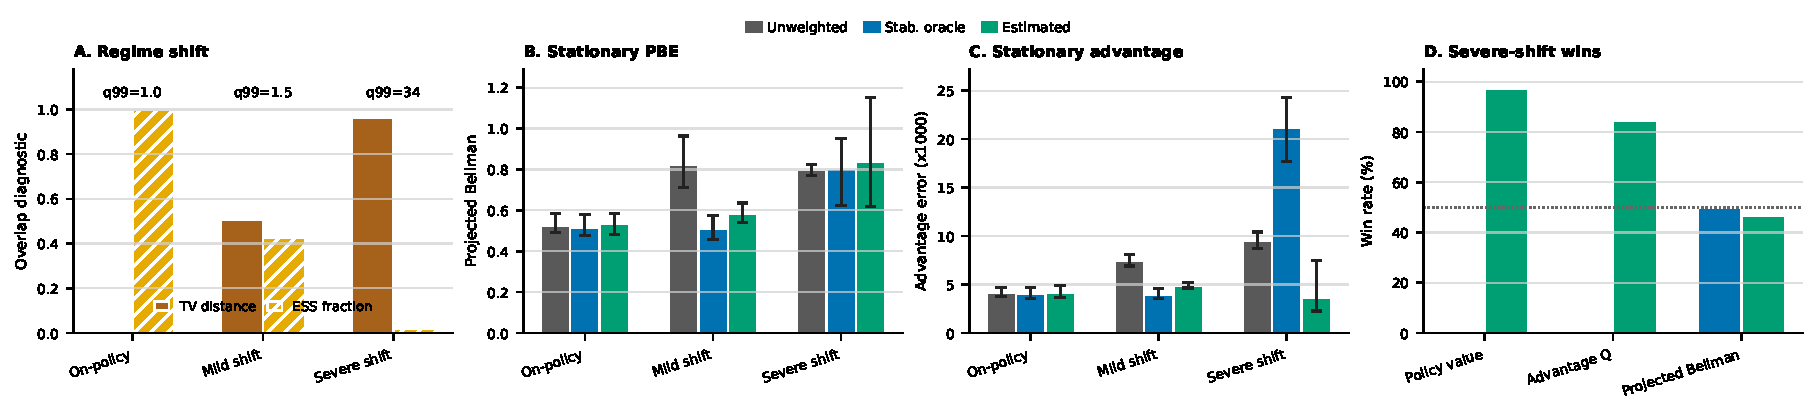
\includegraphics[width=\linewidth]{figures/main_text_simulation_figure.pdf}
\caption{Continuous offline RL. (A) Overlap diagnostics over ten behavior
regimes from near-on-policy to severe off-policy shift. (B) Stationary
projected Bellman error. (C) Advantage-centered stationary \(Q\)-error. (D)
Severe-shift win rates against unweighted soft FQI; unweighted is the reference.
Points and intervals in (B)--(C) show medians and IQRs over 500 datasets.}
\label{fig:soft-fqi-main}
\end{figure}

Figure~\ref{fig:soft-fqi-main} reports stationary projected Bellman error,
\(\|Q-\mathcal T_{\mathcal F}(Q)\|_{2,\mu^\star}\), and
advantage-centered stationary \(Q\)-RMSE,
\(\|(Q-Q^\star_\tau)-\pi^\star(Q-Q^\star_\tau)\|_{2,\mu^\star}\), which removes
within-state shifts and captures action-relevant error. Weighting is neutral
near on-policy but reduces target-stationary Bellman and advantage errors as
behavior--target shift increases. Under severe shift, poor coverage makes exact
ratios highly variable, so stabilized approximate weighting can improve
action-relevant error even when it does not uniformly reduce projected Bellman
error. Estimated local RBF-polynomial weights beat unweighted FQI on advantage
error in 407 of 500 seeds and policy value in 488 of 500 seeds, but on
projected Bellman residual in only 234 of 500 seeds. Expanded discussion is in
Appendix~\ref{appendix::contexp}.

\textbf{Comparison with minimax Bellman-residual fitting.}
Appendix~\ref{appendix::minimax} compares stationary weighting with a
regularized minimax Bellman-residual baseline using the same linear
\(Q\)-features and the same RBF-polynomial critic dictionary used for ratio
estimation. The methods show complementary strengths: estimated stationary
weights track the stabilized oracle correction when coverage is adequate, while
minimax residual fitting is competitive in some severe-shift regimes where
ratio estimation is difficult. We evaluate minimax by Bellman residual,
advantage error, and true-\(Q\) error.

\textbf{Takeaway.}
The results suggest that Bellman completeness is not the only route to stable
soft fitted value iteration: aligning the projection norm with the local
stationary geometry can recover contraction under misspecification. The
guarantees remain local and finite-action. In particular, constants depend on
minimum action probabilities, the present proof does not directly cover
continuous actions, and without an action gap the low-temperature contraction
radius can shrink. High-dimensional offline RL benchmarks are left for future
work.


\FloatBarrier
\bibliographystyle{plainnat}
\bibliography{../../common/ref}








 \appendix
\section{Discussion and Conclusion}
\label{app:additional-conclusion}

This paper identifies a simple mechanism behind the stability of fitted soft
value iteration without Bellman completeness. Near the soft-optimal fixed point,
the soft Bellman operator behaves like policy evaluation under the soft-optimal
policy, whose natural contraction norm is the corresponding stationary
state-action norm. Standard off-policy soft FQI instead projects Bellman targets
in the behavior norm. Under function approximation and distribution shift, this
projection-norm mismatch can destroy the local contraction that would otherwise
stabilize fitted iteration.

Stationary reweighting addresses this mismatch without changing the Bellman
target, adding an adversarial critic, or imposing Bellman completeness. It
changes only the regression weights, so that the fitted projection approximates
the stationary projection suggested by the local dynamics. Our finite-sample
analysis shows that, inside a contraction basin, the iterates converge linearly
to the stationary projected fixed point up to statistical and weight-estimation
errors. The bound also clarifies how approximate weights enter: they affect the
regression curvature and interact with the Bellman approximation residual, so
imperfect weights are less harmful when the function class is closer to Bellman
complete.

The result is local, and its scope is determined by basin entry, coverage, and
weight estimation. Stationary weighting requires sufficient overlap between the
behavior distribution and the relevant stationary distribution, and poor overlap
can make exact ratios too variable. This motivates regularized, discounted,
clipped, or otherwise stabilized occupancy weights in practice, as well as warm
starts and temperature annealing as basin-entry strategies. These requirements
reflect the usual coverage and stability challenges in off-policy value
learning, rather than a limitation specific to stationary reweighting.

Stationary weighting should be viewed as complementary to minimax and
adversarial Bellman-residual methods. Minimax objectives provide a powerful way
to control Bellman residuals through critic classes and can perform well with
suitable tuning. Stationary weighting offers a different route: it preserves the
supervised-regression structure of FQI while aligning the fitted objective with
the distribution under which the local Bellman dynamics contract. Understanding
how these approaches can be combined, and how to tune them reliably under
limited overlap, is an important direction for future work.

Overall, the main message is that Bellman completeness is not the only way to
control fitted soft value iteration. When the projection norm is aligned with
the stationary geometry of the target policy, local contraction can be recovered
under misspecification. This perspective makes the role of coverage explicit,
explains when ordinary soft FQI is already stable, and provides a modular path
for stabilizing regression-based offline RL with existing density-ratio and
balancing-weight tools.

 

\section{Main experiment results}
\subsection{Illustrative Garnet experiment}
\label{appendix::expgarnet}
We generate Garnet MDPs \citep{bhatnagar2009natural} with
\(|\mathcal S|=50\), \(|\mathcal A|=4\), branching factor \(5\), and
\(\gamma=0.99\). The target is the near-hard-max soft-optimal policy at
\(\tau=10^{-6}\), while the behavior policy is drawn independently at each
state, creating severe norm mismatch. We use a five-dimensional linear class
that contains \(Q^\star_\tau\) but is not Bellman complete: in each seed, the
first basis vector is the normalized \(Q^\star_\tau\) table and the remaining
four basis vectors are independent Gaussian state-action features orthogonalized
against it. We collect \(10^5\) reset-sampled one-step transitions.
Figure~\ref{fig:soft-fqi-garnet}
shows the mechanism cleanly: under low temperature, behavior-distribution-norm FQI can be
unstable; stationary weighting stabilizes the projected dynamics; and
annealing improves the trajectory into the low-temperature regime.

\begin{figure}[h]
    \centering
    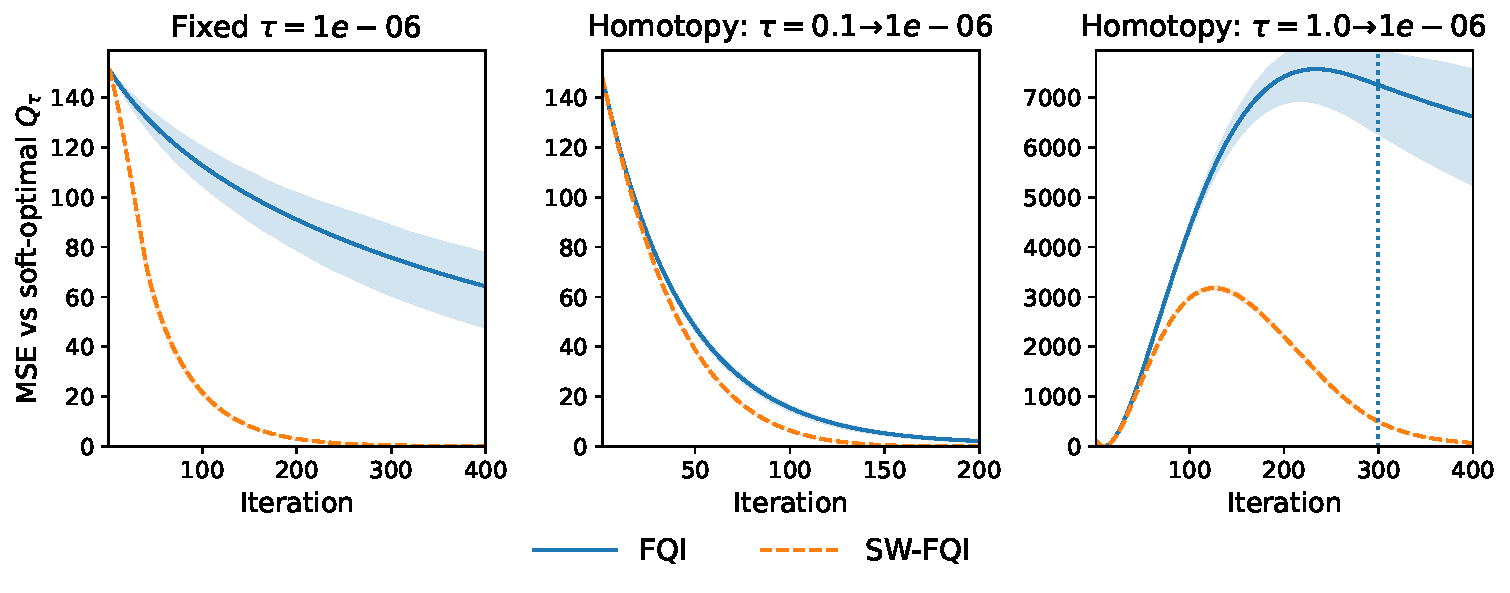
\includegraphics[width=0.7\linewidth]{figures/soft_fqi_garnet_benchmark_5b.pdf}
    \caption{Illustrative Garnet diagnostic. Left: direct training at
    \(\tau=10^{-6}\). Middle/right: temperature homotopy. Shaded regions show
    25\%--75\% quantiles over 200 random MDPs/datasets; the dashed line marks
    when \(\tau\) reaches its target.}
    \label{fig:soft-fqi-garnet}
\end{figure}


\subsection{Continuous offline RL}
\label{appendix::contexp}

\textbf{Expanded setup.}
We evaluate a continuous-state navigation MDP designed to separate Bellman
incompleteness from off-policy distribution shift. The environment has five
actions, nonlinear stochastic dynamics, a goal region, and a decoy region that
attracts behavior data. A grid solve at \(\tau=10^{-3}\) gives
\(Q^\star_\tau\), the target stationary distribution, and oracle density ratios.
Across ten behavior regimes, from nearly on-policy to severe shift, we run 60
iterations with a deliberately Bellman-incomplete linear state-action
\(Q\)-class, comparing unweighted soft FQI, stabilized oracle stationary
weighting, and estimated local RBF-polynomial stationary weighting. Both
weighted methods clip and renormalize positive weights and mix toward uniform
weights when effective sample size is too small. The estimated method uses a
DICE-style saddle-point moment estimator with a shared RBF-polynomial dictionary
and a discounted target \((\gamma_w=0.95)\) instead of the exact stationary
target. We report direct low-temperature fitting at \(\tau=10^{-3}\);
Appendix~\ref{app:soft-fqi-simulation-details} gives details and annealing
comparisons, which gave modest but consistent improvements.


\textbf{Expanded discussion.} Figure~\ref{fig:soft-fqi-main} In Appendix \ref{appendix::contexp} reports stationary projected Bellman error
\(\|Q-\mathcal T_{\mathcal F}(Q)\|_{2,\mu^\star}\), which vanishes at the
projected fixed point \(Q^\dagger\), and advantage-centered stationary
\(Q\)-RMSE,
\(\|(Q-Q^\star_\tau)-\pi^\star(Q-Q^\star_\tau)\|_{2,\mu^\star}\), which removes
constant shifts and captures policy-relevant value error. On policy, weighting
is essentially neutral. As shift increases, unweighted FQI has larger
target-stationary Bellman and advantage errors, while weighting reduces these
errors in this controlled setting. Under severe shift, poor coverage makes
exact stationary ratios highly variable, creating a bias--variance tradeoff
between exact and stabilized approximate reweighting. Estimated local
RBF-polynomial weights improve the policy-relevant quantities in most seeds:
they beat unweighted FQI on advantage error in 407 of 500 seeds and policy value
in 488 of 500 seeds. This does not uniformly translate to projected Bellman
residual, where estimated weights beat unweighted FQI in 234 of 500 seeds. Thus
stable approximate weighting can improve policy quality under limited coverage
even when it does not uniformly reduce projected Bellman error.




The main figure for the continuous offline RL experiment is
Figure~\ref{fig:soft-fqi-main}.


 



\subsection{Minimax Bellman-residual comparison}
\label{appendix::minimax}

\textbf{Expanded comparison with minimax Bellman-residual fitting.}
We compare stationary weighting with a regularized minimax Bellman-residual
baseline using the same linear \(Q\)-features as soft FQI and the same
RBF-polynomial critic dictionary used for ratio learning. This gives a strong
residual-minimization comparator without changing the actor's approximation
class. Figure~\ref{fig:minimax-weighting-overlap} reports policy-relevant
advantage error, unprojected target-stationary Bellman residual, and
target-stationary \(Q\)-error, evaluating minimax on its natural residual metric
and on the \(Q\)- and advantage-level quantities used in the main analysis.
Estimated stationary weights track the stabilized oracle correction when
coverage is adequate; minimax fitting is more competitive in severe-shift
regimes where ratio estimation is difficult.
Figure~\ref{fig:softfqi-minimax-oracle-sensitivity} and
Table~\ref{tab:oracle-tuned-tikhonov} in Appendix~\ref{app:soft-fqi-simulation-details} show that heavier Tikhonov regularization
can improve the minimax residual while leaving substantial target-stationary
\(Q\)-error.

 
\begin{figure}[h]
\centering
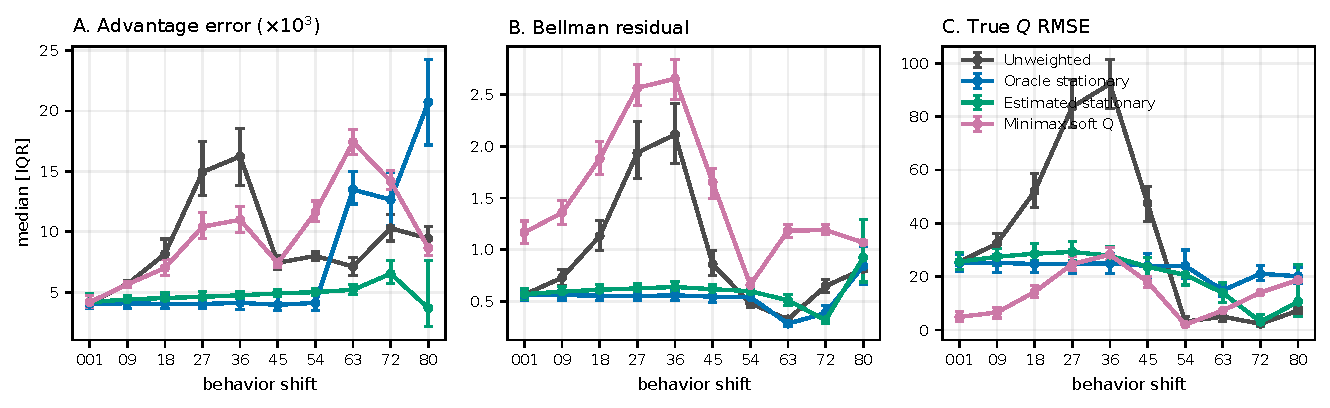
\includegraphics[width=\linewidth]{figures/minimax_vs_weighting_overlap_regimes.pdf}
\caption{Minimax Bellman-residual comparison. We compare unweighted soft FQI,
stabilized-oracle stationary weighting, estimated stationary weighting, and a
Tikhonov-regularized minimax Bellman-residual baseline over the same ten
behavior regimes. Points and intervals show medians and IQRs over 500 datasets.
The panels report target-stationary advantage error, the unprojected
target-stationary Bellman residual, and target-stationary \(Q\)-error.}
\label{fig:minimax-weighting-overlap}
\end{figure}



 

\section{Controlled simulation details}
\label{app:soft-fqi-simulation-details}

\paragraph{Environment and grid reference.}
The benchmark is a continuous two-dimensional navigation MDP with five
discrete actions, nonlinear stochastic dynamics, a high-reward goal basin, and
a lower-reward decoy basin. The decoy is used only to construct behavior
policies whose stationary distributions differ from the soft-optimal stationary
distribution. We compute reference quantities on a grid: soft value iteration
with temperature \(\tau=10^{-3}\) gives \(Q^\star_\tau\), the soft-optimal
policy, and the corresponding stationary state-action distribution. Oracle
density ratios are the soft-optimal stationary probabilities divided by the
behavior stationary probabilities.
The state space is the box \([-1,1]^2\), discretized as a \(25\times25\) grid
for reference dynamic programming. The five action vectors are
\((0,0)\), \((0.23,0)\), \((-0.23,0)\), \((0,0.23)\), and \((0,-0.23)\). For
state \(s=(x,y)\) and action \(a=(a_x,a_y)\), the transition mean before
clipping to the box is
\[
s
+0.13
\begin{pmatrix}
\sin(\pi y)+0.35x(1-y^2)\\
-0.85\sin(\pi x)+0.25y(1-x^2)
\end{pmatrix}
+a
+0.055
\begin{pmatrix}
a_y x\\
-a_x y
\end{pmatrix}.
\]
The grid transition probabilities are proportional to a Gaussian density around
this mean with standard deviation \(0.075\), mixed with uniform teleportation
probability \(0.002\). Rewards are evaluated at the transition mean:
\[
\begin{aligned}
r(s,a)
=\;&1.20\,b_{(0.62,0.62),0.20}
+0.55\,b_{(-0.55,0.45),0.23}
-0.22\,b_{(0.05,-0.10),0.22}
\\
&-0.035\frac{\|a\|_2^2}{0.23^2}
+0.055\{\sin(2\pi x)a_x-\cos(\pi y)a_y\},
\end{aligned}
\]
where \(b_{c,\sigma}(z)=\exp\{-\|z-c\|_2^2/(2\sigma^2)\}\). Each finite-sample
run uses \(n=5000\) one-step transitions, discount \(\gamma=0.97\), 60 FQI
iterations, and ridge \(10^{-4}\). The main direct/annealed comparison uses 500
seeds, and the oracle annealing sensitivity uses 200 seeds.

\paragraph{Behavior regimes.}
Only the data-collection distribution changes across regimes. We use ten
mixtures ranging from
\(0.999\pi^\star+0.001\pi_{\mathrm{unif}}\) to
\(0.20\pi^\star+0.70\pi_{\mathrm{decoy}}+0.10\pi_{\mathrm{unif}}\), with
intermediate target-policy masses \(0.91,0.82,\ldots,0.28\). The mild-shift
regime,
\(0.55\pi^\star+0.35\pi_{\mathrm{decoy}}+0.10\pi_{\mathrm{unif}}\), has total
variation distance \(0.507\), ESS fraction \(0.428\), and 99th percentile
oracle ratio \(1.5\). The most severe regime has total variation distance
\(0.964\), ESS fraction \(0.017\), and 99th percentile oracle ratio \(34\).

For each behavior regime, we report two overlap diagnostics. The total
variation distance is
\[
\mathrm{TV}(\mu^\star,\nu_b)
=
\frac12\sum_{s,a}\left|\mu^\star(s,a)-\nu_b(s,a)\right|,
\]
where \(\mu^\star\) is the soft-optimal stationary state-action distribution and
\(\nu_b\) is the behavior stationary state-action distribution. The effective
sample size fraction is the population oracle-ratio quantity
\[
\mathrm{ESS}
=
\frac{1}{E_{\nu_b}[(d^\star)^2]},
\qquad
d^\star=\frac{d\mu^\star}{d\nu_b},
\]
the population analogue of \((\sum_i w_i)^2/(n\sum_i w_i^2)\).

\paragraph{Weight stabilization and estimated stationary weights.}
The stabilized oracle method starts from the grid-computed stationary density
ratio to the fixed soft-optimal reference policy \(\pi^\star_\tau\). In the
experiments the weighted regressions use this fixed target/reference weight
rather than refitting a new ratio for every FQI iterate. The estimated local
RBF-polynomial method uses the same state-action samples as FQI. The linear
\(Q\)-class has ten features
\[
1,\ x,\ y,\ a_x,\ a_y,\ x^2,\ y^2,\ a_x^2+a_y^2,\ 
b_{(0.62,0.62),0.28}(s),\ b_{(-0.55,0.45),0.30}(s).
\]
The ratio and critic share a finite RBF-polynomial dictionary consisting of ten
polynomial state-action features plus \(36\) state centers crossed with five
actions, for \(190\) total features. The RBF bandwidth is \(0.65\) times the
median positive distance between dictionary centers. The DICE-style estimator
uses primal and dual ridge penalties \(10^{-5}\) and normalization penalty
10. We target discounted stationary ratios with \(\gamma_w=0.95\), which
regularizes the stationary-flow equations while keeping the weights close to
the stationary correction. For both weighted methods, raw weights are truncated
below at \(10^{-8}\), clipped at the smaller of the empirical 99th percentile
and 25, renormalized to have mean one, and mixed as
\((1-\lambda)w+\lambda\). We choose \(\lambda\in[0,0.50]\) by binary search to
raise the empirical ESS fraction to at least \(0.25\) when possible, using
\(\lambda=0.50\) otherwise.

\paragraph{Diagnostics.}
Stationary projected Bellman error is the Bellman residual after projection in
the target stationary norm. Advantage-centered stationary \(Q\)-error subtracts
the within-state action average before computing target-stationary error,
removing raw \(Q\)-shifts that do not affect low-temperature action choice.
Panel~D reports severe-shift win rates against unweighted FQI for the three
diagnostics shown or discussed in the main text.

\paragraph{Minimax Bellman-residual baseline.}
The minimax comparison uses the same \(Q\)-function class as the corresponding
soft FQI run. For a linear parameterization \(Q_\theta\), let
\(\delta_\theta(S,A,R,S')\) denote the soft Bellman residual formed with the
same target update and temperature as the fitted-\(Q\) regressions. The critic
class is the same RBF-polynomial dictionary \(\psi(S,A)\) used by the
stationary-ratio estimator. The baseline solves the regularized empirical
projected-residual objective
\[
  \min_\theta
  \left\|
    \mathbb P_n \psi\,\delta_\theta
  \right\|_{(\mathbb P_n\psi\psi^\top+\lambda_c I)^{-1}}^2
  + \lambda_q\|\theta\|_2^2 ,
\]
with \(\lambda_q=\lambda_c=10^{-4}\) unless otherwise stated. We also ran a
ridge-sensitivity check over
\[
10^{-6},3\cdot10^{-6},10^{-5},3\cdot10^{-5},10^{-4},
3\cdot10^{-4},10^{-3},3\cdot10^{-3},10^{-2},3\cdot10^{-2},10^{-1},
\]
and a cross-validated ridge choice using the same ridge family as the ratio
estimator. The estimated-weight ablation likewise includes fixed-ridge and
cross-validated Tikhonov choices. Thus the comparison does not give stationary
weighting a larger \(Q\)-class; it compares two ways of stabilizing fitted
Bellman updates, either by changing the regression geometry through stationary
weights or by controlling Bellman moments with an adversarial residual critic.

\paragraph{Additional stress tests.}
We include three diagnostics to separate the proposed mechanism from generic
regularization effects. First, a rich-feature negative control augments the
linear action features with RBF state-action features, substantially reducing
projection mismatch. In the mild and moderate regimes, the gains from
stationary weighting become modest, as expected if weighting mainly corrects
the projection geometry rather than acting as a generic regularizer; the
severe-shift case remains coverage-limited. Second, a sample-size sweep varies
the number of behavior transitions from \(1000\) to \(10000\) in three shift
regimes. The estimated-weight gap to oracle weighting shrinks as effective
sample size improves, while the most severe regimes remain limited by coverage.
Third, a weight-estimator ablation varies the discounted stationary target
\(\gamma_w\in\{0,0.5,0.95,1\}\) and compares fixed-ridge and cross-validated
ridge choices. The ablation shows the expected bias--variance tradeoff: nearly
stationary targets can be accurate when coverage is adequate, while discounted
or ridge-stabilized targets are more reliable under severe shift.

\begin{figure}[t]
\centering
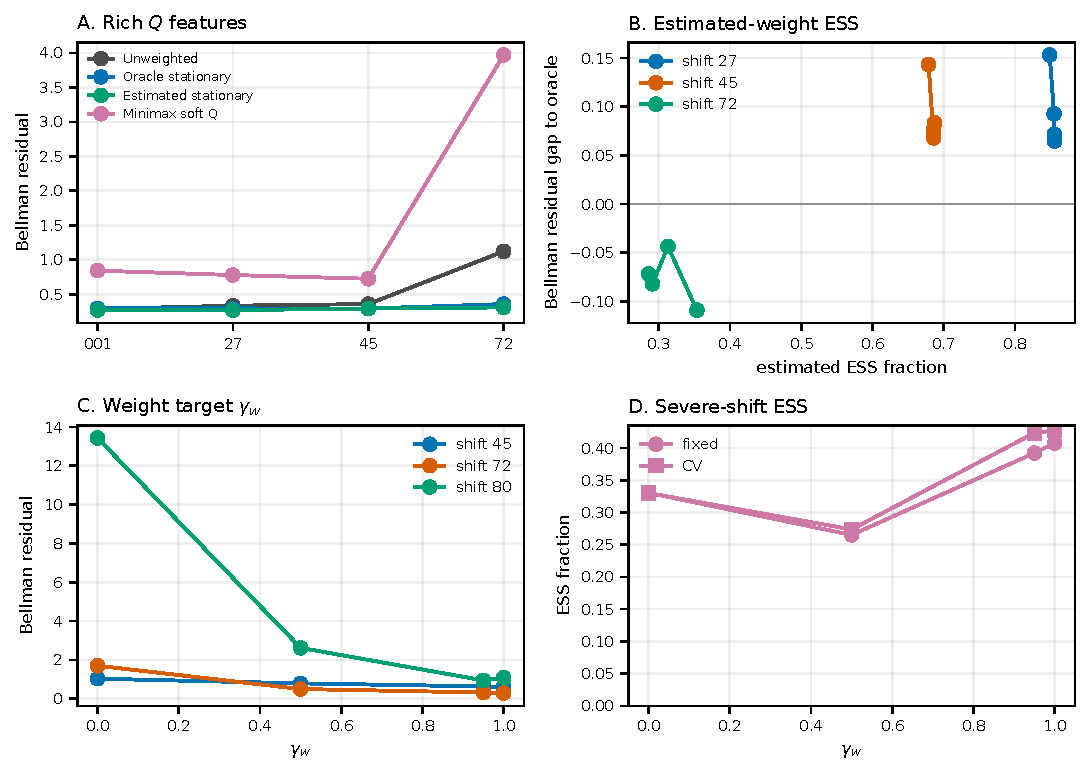
\includegraphics[width=\linewidth]{figures/softfqi_supporting_diagnostics.pdf}
\caption{\textbf{Supporting diagnostics.} Richer \(Q\)-features reduce the
weighting gap in the mild and moderate regimes, while the severe-shift case
remains coverage-limited. The ESS and \(\gamma_w\) sweeps show when estimated
stationary weights track the oracle correction and when finite-sample weight
error dominates.}
\label{fig:softfqi-supporting-diagnostics}
\end{figure}

\begin{figure}[t]
\centering
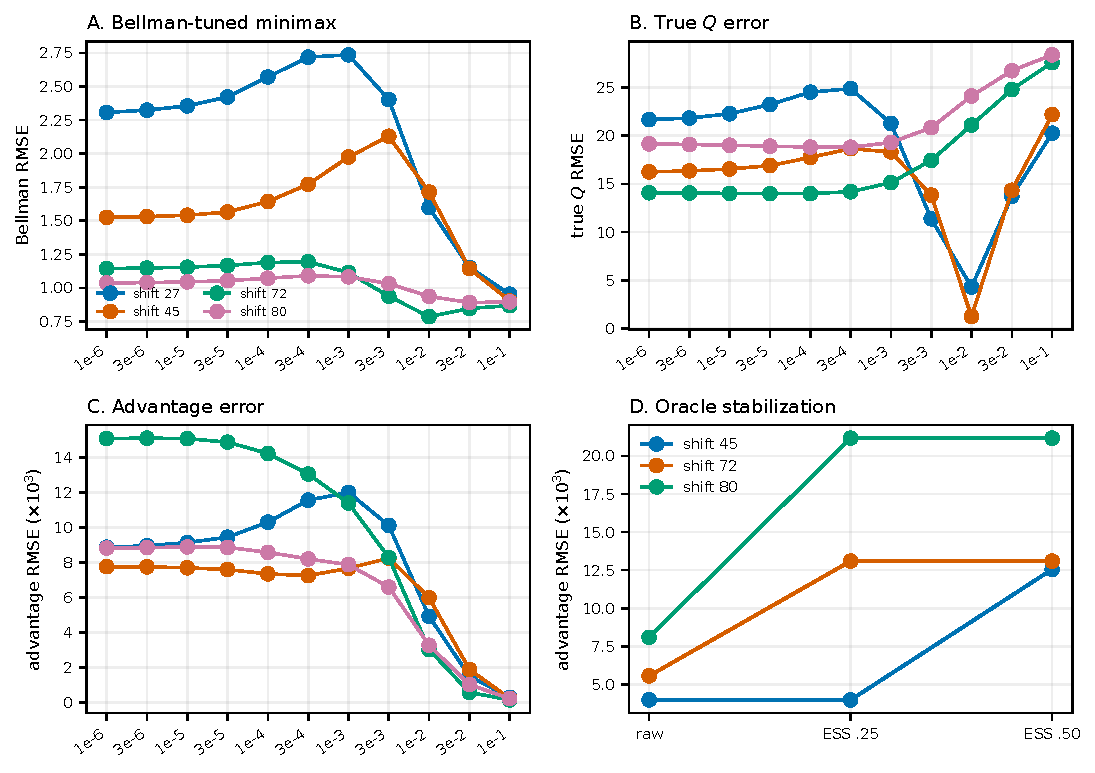
\includegraphics[width=\linewidth]{figures/softfqi_minimax_oracle_sensitivity.pdf}
\caption{\textbf{Minimax and oracle-stabilization sensitivity.} Varying the
minimax ridge reveals the residual--shrinkage tradeoff: stronger regularization
can reduce Bellman residuals and advantage error while still leaving large
target-stationary \(Q\)-error. Oracle stabilization controls the severe-shift
bias--variance tradeoff for exact stationary ratios.}
\label{fig:softfqi-minimax-oracle-sensitivity}
\end{figure}

\begin{figure}[t]
\centering
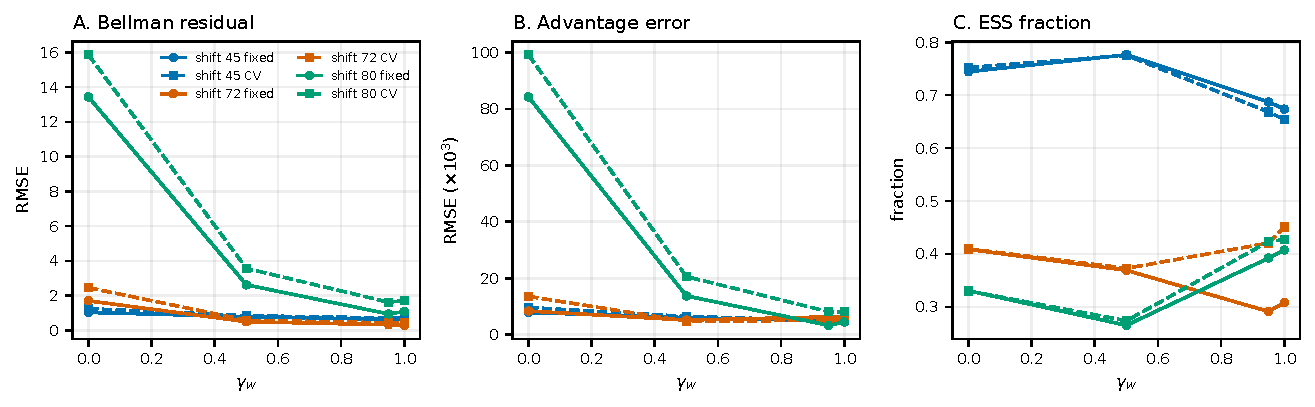
\includegraphics[width=\linewidth]{figures/softfqi_weight_estimator_sensitivity.pdf}
\caption{\textbf{Estimated-weight sensitivity.} We vary the stationary target
\(\gamma_w\) and compare fixed versus cross-validated Tikhonov regularization
for the density-ratio estimator. The severe-shift regimes show the expected
bias--variance tradeoff: more target-stationary weights improve the residual
when coverage is adequate, while ESS and ridge selection determine stability.}
\label{fig:softfqi-weight-estimator-sensitivity}
\end{figure}

\paragraph{Oracle tuning check.}
Table~\ref{tab:oracle-tuned-tikhonov} gives a deliberately generous tuning
check. For each family and regime, we select the Tikhonov setting, and for
estimated weights also the stationary target \(\gamma_w\), that minimizes the
target-stationary Bellman residual after observing the true grid reference. This
is not a deployable model-selection rule; it is a sensitivity analysis to check
that the comparison is not an artifact of the default ridge. Oracle tuning
improves residuals for both families in some regimes, but heavily regularized
minimax fits can still have large true-\(Q\) error. The qualitative pattern is
unchanged: minimax remains a useful Bellman-residual baseline, while stationary
weighting more directly targets the target-stationary \(Q\) geometry.

\begin{table}[t]
\centering
\caption{Oracle-tuned Tikhonov sensitivity for estimated stationary weights and
minimax soft \(Q\). Entries are medians with interquartile ranges over the
corresponding sweep. The oracle criterion column indicates which metric was
used to choose the tuning rule within each family and regime.}
\label{tab:oracle-tuned-tikhonov}
\scriptsize
\resizebox{\linewidth}{!}{\begin{tabular}{llllllll}
\toprule
family & regime & oracle criterion & selected Tikhonov/target & Bellman RMSE & Advantage x1e3 & True Q RMSE & Value error \\
\midrule
estimated weights & shift 45 & Bellman RMSE & $\gamma_w=1$, fixed, $\lambda=1e-05$ & 0.614 [0.555, 0.654] & 4.97 [4.69, 5.24] & 22.1 [18.8, 25.6] & 25.6 [25.6, 25.6] \\
estimated weights & shift 72 & Bellman RMSE & $\gamma_w=1$, fixed, $\lambda=1e-05$ & 0.291 [0.27, 0.326] & 6.55 [5.67, 7.51] & 2.49 [1.22, 4.86] & 25.6 [25.6, 27.3] \\
estimated weights & shift 80 & Bellman RMSE & $\gamma_w=0.95$, fixed, $\lambda=1e-05$ & 0.946 [0.715, 1.21] & 3.32 [2.36, 6.91] & 10.6 [4.45, 20.7] & 25.6 [25.6, 27.1] \\
minimax soft Q & shift 27 & Bellman RMSE & $\lambda_q=\lambda_c=10^{-1}$ & 0.953 [0.951, 0.956] & 0.282 [0.279, 0.287] & 20.3 [20.1, 20.4] & 25.6 [25.6, 25.6] \\
minimax soft Q & shift 45 & Bellman RMSE & $\lambda_q=\lambda_c=10^{-1}$ & 0.903 [0.901, 0.905] & 0.222 [0.215, 0.226] & 22.2 [22.1, 22.3] & 25.6 [25.6, 25.6] \\
minimax soft Q & shift 72 & Bellman RMSE & $\lambda_q=\lambda_c=10^{-2}$ & 0.786 [0.782, 0.792] & 3.02 [2.94, 3.11] & 21.1 [20.7, 21.4] & 25.6 [25.6, 25.6] \\
minimax soft Q & shift 80 & Bellman RMSE & $\lambda_q=\lambda_c=3\times 10^{-2}$ & 0.891 [0.889, 0.893] & 1.02 [0.99, 1.04] & 26.7 [26.7, 26.8] & 27.3 [27.3, 27.3] \\
\bottomrule
\end{tabular}
}
\end{table}

\paragraph{Annealing sensitivity.}
The main continuous experiment uses direct low-temperature fitting at
\(\tau=10^{-3}\). To check whether continuation becomes more important near the
hard-max limit, we also repeat the experiment at \(\tau=10^{-6}\). For
\(\tau=10^{-3}\), we use the staged schedule
\(0.2,0.05,0.01,0.003,10^{-3}\); for \(\tau=10^{-6}\), we append a final
\(10^{-6}\) stage. Table~\ref{tab:soft-fqi-annealing-sensitivity} reports
median stationary projected Bellman error over 200 datasets. Annealing has a
small effect at both temperatures: the largest median change is \(1.26\%\) at
\(\tau=10^{-3}\) and \(1.21\%\) at \(\tau=10^{-6}\).

\begin{table}[h]
\centering
\caption{Annealing sensitivity. Entries are median stationary projected
Bellman error over 200 offline datasets. Gain is
\((\mathrm{direct}-\mathrm{annealed})/\mathrm{direct}\).}
\label{tab:soft-fqi-annealing-sensitivity}
\begin{tabular}{lllccc}
\toprule
\(\tau\) & Regime & Method & Direct & Annealed & Gain \\
\midrule
\(10^{-3}\) & On-policy & Unweighted & 0.526 & 0.521 & 0.94\% \\
\(10^{-3}\) & On-policy & Stab.\ oracle & 0.516 & 0.510 & 1.05\% \\
\(10^{-3}\) & On-policy & Estimated & 0.533 & 0.527 & 1.05\% \\
\(10^{-3}\) & Mild shift & Unweighted & 0.822 & 0.819 & 0.37\% \\
\(10^{-3}\) & Mild shift & Stab.\ oracle & 0.510 & 0.504 & 1.10\% \\
\(10^{-3}\) & Mild shift & Estimated & 0.584 & 0.577 & 1.17\% \\
\(10^{-3}\) & Severe shift & Unweighted & 0.798 & 0.788 & 1.26\% \\
\(10^{-3}\) & Severe shift & Stab.\ oracle & 0.804 & 0.797 & 0.80\% \\
\(10^{-3}\) & Severe shift & Estimated & 0.839 & 0.832 & 0.82\% \\
\(10^{-6}\) & On-policy & Unweighted & 0.529 & 0.524 & 0.94\% \\
\(10^{-6}\) & On-policy & Stab.\ oracle & 0.519 & 0.515 & 0.80\% \\
\(10^{-6}\) & On-policy & Estimated & 0.533 & 0.529 & 0.79\% \\
\(10^{-6}\) & Mild shift & Unweighted & 0.811 & 0.808 & 0.38\% \\
\(10^{-6}\) & Mild shift & Stab.\ oracle & 0.508 & 0.504 & 0.85\% \\
\(10^{-6}\) & Mild shift & Estimated & 0.581 & 0.574 & 1.09\% \\
\(10^{-6}\) & Severe shift & Unweighted & 0.798 & 0.789 & 1.21\% \\
\(10^{-6}\) & Severe shift & Stab.\ oracle & 0.815 & 0.809 & 0.83\% \\
\(10^{-6}\) & Severe shift & Estimated & 0.849 & 0.845 & 0.42\% \\
\bottomrule
\end{tabular}
\end{table}

\section{Local Geometry and Operator Smoothness}
\label{app:local-geometry-operator-smoothness}

This appendix collects the local contraction picture and the operator-smoothness facts used to prove the local contraction theorem.

\subsection{Local contraction geometry}
\label{app:local-geometry}

Figure~\ref{fig:local-geometry} summarizes the geometry behind the local
contraction argument. Inside \(\mathbb B_{\mathcal F}(r_{\mathrm{loc}},Q^\star)\), the Bellman map
\(\mathcal T\) contracts toward \(Q^\star\), while the projection
\(\Pi_{\mathcal F}\) keeps iterates in \(\mathcal F\). Starting in
\(\mathbb B_{\mathcal F}(r,Q^\dagger)\) with
\(r+\varepsilon_{\mathcal F}<r_{\mathrm{loc}}\), the iterates remain
inside the contraction region and move toward the constrained fixed point
\(Q^\dagger\).

\begin{figure}[t]
    \centering
% Shared radii (ensures alignment across both figures)
\def\R{2.4}   % corresponds to r_{\mathrm{loc}}
\def\r{1.5}   % corresponds to an admissible r

\begin{tikzpicture}[scale=0.9, >=Stealth]

  % Centers
  \coordinate (Qstar)  at (0,0);
  \coordinate (QFstar) at ({\R-\r},0); % tangent inside

  % Outer circle: contraction region
  \draw[thick] (Qstar) circle (\R);

  % Text label + math label (bottom, inside)
  \node at ($(Qstar)+(90:0.8*\R)$) {
    \begin{tabular}{c}
      \small $\mathbb{B}_{\mathcal F}(r_{\mathrm{loc}},\, Q^\star)$
    \end{tabular}
  };

  % Inner circle: basin of attraction
  \draw[thick, dashed] (QFstar) circle (\r);

  % Basin label (top, inside)
  \node at ($(QFstar)+(90:0.9)$) {
    \begin{tabular}{c}
      \small $\mathbb{B}_{\mathcal F}(r,\, Q^\dagger)$
    \end{tabular}
  };

  % Points
  \fill (Qstar) circle (2pt);
  \fill (QFstar) circle (2pt);

  % Labels
  \node[below, xshift=-5pt] at (Qstar) {$Q^\star$};
  \node[below, xshift=12pt, yshift=10] at (QFstar) {$Q^\dagger$};

\draw[-, thick] (Qstar) -- (QFstar)
     node[midway, above] {\scriptsize $\varepsilon_{\mathcal F}$};

  % Contraction point inside basin (below + right)
  \coordinate (Qtemp) at ($(QFstar)+(-50:0.9*\r)$);

  % Draw point Q (label above so it's inside the circle)
  \fill (Qtemp) circle (2pt);
  \node[above] at (Qtemp) {\small $Q$};

% Dashed contraction arrow toward Q_F^*
\draw[->, dashed, thick]
    (Qtemp) -- ($(QFstar)!0.065!(Qtemp)$)
      node[midway, below right, xshift=-2pt, yshift=14pt]
           {\scriptsize $\rho_{\mathrm{loc}}(r+\varepsilon_{\mathcal F})$};

% --- Extra arrowhead in the same direction ---

% Compute inner point on the main arrow
\coordinate (innerF)   at ($(QFstar)!0.05!(Qtemp)$);

% Midpoint between Qtemp and innerF
\coordinate (midF)     at ($(Qtemp)!0.5!(innerF)$);

% Draw a tiny arrow segment in the same direction
\draw[-{Stealth[scale=0.8]}, dashed, thick]
    (midF) -- ($(midF)!0.15!(innerF)$);

% Main dashed contraction arrow toward true Q^*
\draw[->, dashed, thick]
    (Qtemp) -- ($(Qstar)!0.05!(Qtemp)$)
      node[midway, below right, xshift=-22pt, yshift=-1pt]
           {\scriptsize $\rho_{\mathrm{loc}}(R)$};

% Compute inner and midpoint along same line
\coordinate (inner)   at ($(Qstar)!0.05!(Qtemp)$);
\coordinate (midStar) at ($(Qtemp)!0.5!(inner)$);

% Small arrow, along same direction, slightly larger head
\draw[-{Stealth[scale=0.8]}, dashed, thick]
    (midStar) -- ($(midStar)!0.15!(inner)$);

\end{tikzpicture}\begin{tikzpicture}[scale=0.9, >=Stealth]

  % Axes (shorter x-axis)
  \draw[->] (-2,0) -- (2,0) node[right] {$Q$};
  \draw[->] (0,-0.1) -- (0,2.1)
      node[above] {\footnotesize $\mathcal{T}(Q)-\mathcal{T}_{\pi^\star}^{\mathrm{eval}}(Q)$};

  % Fixed point Q^*
  \coordinate (Qstar) at (0,0);
  \fill (Qstar) circle (2pt);
  \node[below] at (Qstar) {$Q^\star$};

  % Projected Q_F^*
  \coordinate (QFstar) at ({\R-\r},0);
  \fill (QFstar) circle (2pt);
  \node[below] at (QFstar) {$Q^\dagger$};

  % Curvature |x|^{1+alpha}
  \draw[thick]
    plot[domain=0:1.75, samples=120]
      ({-\x}, {0.6*pow(\x,1.5)});
  \draw[thick]
    plot[domain=0:1.75, samples=120]
      ({\x}, {0.6*pow(\x,1.5)});

  % curvature label
  \node at (0,1)
      {\small $\propto \omega_{\mathcal T}(|x|)\,|x|$};

\end{tikzpicture}

\captionsetup{aboveskip=2pt, belowskip=0pt}
\caption{Contraction geometry. Left: contraction region
$\mathbb{B}_{\mathcal F}(r_{\mathrm{loc}}, Q^\star)$ and basin of attraction
$\mathbb{B}_{\mathcal F}(r, Q^\dagger)$, where
$r+\varepsilon_{\mathcal F}<r_{\mathrm{loc}}$.
Right: one--dimensional curvature slice of
$\mathcal{T}(Q)-\mathcal{T}_{\pi^\star}^{\mathrm{eval}}(Q)$
near $Q^\star$, with distances
$R = \mathrm{dist}(Q, Q^\star)$ and
$r = \mathrm{dist}(Q, Q^\dagger)$.}
\label{fig:local-geometry}
\vspace{-4pt}
\end{figure}

\subsection{Operator smoothness results}

 \subsubsection{First derivative of the Bellman operator}


\begin{lemma}[First derivative of the soft Bellman operator]
\label{lem:first-derivative}
For any $Q$ and perturbation $H$, the Fréchet derivative of $\mathcal T$ at $Q$
is
\[
D\mathcal T(Q)[H] \;=\; \gamma\,P^{\mathrm{eval}}_{\pi_Q}H.
\]
In particular, at $Q^\star$, $\|D\mathcal T(Q^\star)[H]\|_{2,\mu^\star}
\;\le\;
\gamma\,\|H\|_{2,\mu^\star}$.
\end{lemma}

\begin{proof}[Proof of Lemma~\ref{lem:first-derivative}]
Fix $(s,a)$ and a perturbation $H$. Since the reward term does not depend on $Q$,
\[
D\mathcal{T}(Q)[H](s,a)
=
\gamma\,\E_{S'\sim P(\cdot\mid s,a)}
\big[D\phi_{S'}(Q)[H]\big],
\]
where $\phi_{S'}(Q) := \tau\log\sum_{b}\exp(Q(S',b)/\tau)$.
Let $g(z)=\tau\log\sum_{b}e^{z_b/\tau}$ with $z_b(Q)=Q(S',b)$.
The gradient of $g$ is the softmax, so
$\partial g/\partial z_b(z(Q))=\pi_Q(b\mid S')$.
By the chain rule,
\[
D\phi_{S'}(Q)[H]
=
\sum_{b}\pi_Q(b\mid S')\,H(S',b).
\]
Substituting back gives
\begin{align*}
D\mathcal T(Q)[H](s,a)
&=
\gamma\,\E_{S'\sim P(\cdot\mid s,a)}
\Big[\sum_{b}\pi_Q(b\mid S')\,H(S',b)\Big]
\\[0.3em]
&=
\gamma\,P^{\mathrm{eval}}_{\pi_Q}H(s,a).
\end{align*}
This proves the claim.
\end{proof}



\subsubsection{Second derivative and local curvature}


\textbf{Computation of second derivative.} The next lemma shows that the second derivative of $\mathcal{T}$ has a
positive–semidefinite covariance form.

\begin{lemma}[Second derivative]
\label{lem:second-derivative}
For any $Q$ and directions $H_1, H_2$,
\begin{align*}
&D^2\mathcal{T}(Q)[H_1,H_2](s,a)
=
\\[-0.3em]
&\qquad
\gamma\,\mathbb{E}_{S' \sim P(\cdot \mid s,a)}
\left[
    \tfrac{1}{\tau}\,
    \mathrm{Cov}_{\pi_Q}
    \bigl( H_1(S',\cdot),\, H_2(S',\cdot) \bigr)
\right].
\end{align*}
\end{lemma}

\begin{proof}[Proof of Lemma~\ref{lem:second-derivative}]
Fix $(s,a)$ and directions $H_1,H_2$.  As in
Lemma~\ref{lem:first-derivative},
\begin{align*}
(\mathcal T Q)(s,a)
&=
r_0(s,a)
+
\gamma\,\E_{S'\sim P(\cdot\mid s,a)}
\!\left[\phi_{S'}(Q)\right],\\[0.25em]
\phi_{S'}(Q)
&:=
\tau\log\!\sum_{b}\exp\!\bigl(Q(S',b)/\tau\bigr).
\end{align*}
Thus,
\begin{align*}
&D^2\mathcal T(Q)[H_1,H_2](s,a)\\
\qquad &=
\gamma\,\E_{S'\sim P(\cdot\mid s,a)}
\!\left[
   D^2\phi_{S'}(Q)[H_1,H_2]
\right].
\end{align*}

For fixed $S'$, write $z_b(Q)=Q(S',b)$ and
$g(z)=\tau\log\sum_{b}e^{z_b/\tau}$, so $\phi_{S'}(Q)=g(z(Q))$.
Let $\pi_Q(\cdot\mid S')$ be the softmax at $z(Q)$.
Then
\begin{align*}
\frac{\partial g}{\partial z_b}\bigl(z(Q)\bigr)
&= \pi_Q(b\mid S'),
\\[-0.4em]
\frac{\partial^2 g}{\partial z_b\,\partial z_c}\bigl(z(Q)\bigr)
&=
\frac{1}{\tau}\Bigl[
   \pi_Q(b\mid S')\,\mathbf 1\{b=c\}
\\[-0.4em]
&\hphantom{=\frac{1}{\tau}\Bigl[}\;
   -\,\pi_Q(b\mid S')\,\pi_Q(c\mid S')
\Bigr].
\end{align*}
Hence
\begin{align*}
&  D^2\phi_{S'}(Q)[H_1,H_2]
\\
&\quad =
\sum_{b,c}
\frac{\partial^2 g}{\partial z_b\,\partial z_c}(z(Q))\,
H_1(S',b)\,H_2(S',c)
\\[0.25em]
&\quad =
\frac{1}{\tau}\Bigl(
   \E_{\pi_Q}\!\left[H_1(S',\cdot)\,H_2(S',\cdot)\right]
\\[-0.4em]
&\qquad\qquad\qquad
   -\,\E_{\pi_Q}\!\left[H_1(S',\cdot)\right]\,
      \E_{\pi_Q}\!\left[H_2(S',\cdot)\right]
\Bigr)
\\[0.25em]
&\quad =
\frac{1}{\tau}\,
\Cov_{\pi_Q}\!\bigl(
   H_1(S',\cdot),\,H_2(S',\cdot)
\bigr).
\end{align*}
Taking expectation over $S'$ yields the claimed expression.

\medskip

For positive semidefiniteness, set $H_1 = H_2 = H$:
\begin{align*}
D^2\mathcal T(Q)[H,H](s,a)
&=
\frac{\gamma}{\tau}\,
\E_{S' \sim P(\cdot\mid s,a)}
\Bigl[
   \Var_{\pi_Q}\big(H(S',\cdot)\big)
\Bigr]\\
&\;\ge\; 0.
\end{align*}
In particular, $D^2\mathcal T(Q)$ is positive semidefinite for every $Q$.
Moreover, for any fixed $S'$ the covariance form is strictly positive
whenever $H(S',\cdot)$ is nonconstant under $\pi_Q(\cdot\mid S')$,
so $D^2\mathcal T(Q)$ is strictly positive definite along
nontrivial action-differential directions.
\end{proof}


\textbf{A sufficient interpolation condition.}
The main theorem uses the intrinsic curvature modulus
\(\omega_{\mathcal T}\). The following stronger interpolation condition is a
simple way to verify it in standard classes.
\begin{enumerate}[label=\textbf{S\arabic*)}, ref={S\arabic*}, leftmargin=1.5em]
\item \label{cond::supnorm}
\textbf{\(L^\infty\)--\(L^2\) control.}
There exist \(\alpha\in(0,1]\) and \(C_\infty<\infty\) such that
\[
\|H\|_\infty
\le
C_\infty\|H\|_{2,\mu^\star}^{\alpha}
\]
for all \(H\in\mathcal H_{\mathcal F}^\star\).
\end{enumerate}



\textbf{Uniform boundedness of second derivative and curvature bound.}
\begin{lemma}[Uniform boundedness of the second derivative]
\label{lem:second-derivative-bounded}
Assume Conditions~\ref{cond::posit}–\ref{cond::supnorm} hold. Then there exists a finite constant
\[
\beta_{\loc}
:=
\frac{\gamma}{2\tau}\,
C_{\infty}\sqrt{\frac{|\mathcal{A}|}{\pi_{\min}}}
\]
such that, for all \(Q\), all \(H_2\in L^2(\mu^\star)\), and all
\(H_1=tH\) with \(H\in\mathcal H_{\mathcal F}^\star\) and \(t\in[0,1]\),
\begin{equation}
\label{eq:second-derivative-op-bound}
\bigl\|D^2\mathcal{T}(Q)[H_1,H_2]\bigr\|_{2,\mu^\star}
\;\le\;
\beta_{\loc}\,
\|H_1\|_{2,\mu^\star}^{\alpha}\,
\|H_2\|_{2,\mu^\star},
\end{equation}
where $\alpha$ is the exponent from \ref{cond::supnorm}.
\end{lemma}
\begin{proof}
By Lemma~\ref{lem:second-derivative},
\(D^2\mathcal{T}(Q)[H_1,H_2]\) can be expressed in terms of the covariance
\(\Cov_{\pi_Q}\bigl(H_1(S',\cdot),\, H_2(S',\cdot)\bigr)\).


For fixed $S'$, write $h_i := H_i(S',\cdot)\in\mathbb{R}^{|\mathcal A|}$ and
$p_Q := \pi_Q(\cdot\mid S')$. Then
\[
\Cov_{\pi_Q}\bigl(H_1(S',\cdot),H_2(S',\cdot)\bigr)
=
h_1^\top\bigl(\mathrm{diag}(p_Q) - p_Q p_Q^\top\bigr)h_2,
\]
and the covariance matrix
$\mathrm{diag}(p_Q) - p_Q p_Q^\top$ has spectral norm at most $1/2$, so
\[
\bigl|\Cov_{\pi_Q}\bigl(H_1(S',\cdot),H_2(S',\cdot)\bigr)\bigr|
\;\le\;
\tfrac12\,\|h_1\|_2\,\|h_2\|_2.
\]
Thus, for each $(s,a)$,
\begin{align*}
  &  \bigl|D^2\mathcal{T}(Q)[H_1,H_2](s,a)\bigr|\\
&\;\le\;
\frac{\gamma}{2\tau}\,
\E_{S'\mid s,a}
\bigl[\,\|H_1(S',\cdot)\|_2\,\|H_2(S',\cdot)\|_2\,\bigr].
\end{align*}



Let $(S,A)\sim\mu^\star$ and $S'\sim P(\cdot\mid S,A)$, and define
$Z(S') := \|H_1(S',\cdot)\|_2\,\|H_2(S',\cdot)\|_2$.
By Jensen's inequality,
\begin{align*}
\bigl\|D^2\mathcal{T}(Q)[H_1,H_2]\bigr\|_{2,\mu^\star}^2
&=
\E_{\mu^\star}\Bigl[
  D^2\mathcal{T}(Q)[H_1,H_2](S,A)^2
\Bigr]
\\
&\le
\left(\frac{\gamma}{2\tau}\right)^2
\E_{\mu^\star}
\Bigl[
  \E_{S'\mid S,A} Z(S')^2
\Bigr].
\end{align*}
Since $\mu^\star$ is stationary for $\pi^\star$, the marginal distribution of
$S'$ under $(S,A)\sim\mu^\star$, $S'\sim P(\cdot\mid S,A)$ coincides with the
state marginal of $\mu^\star$. Hence
\[
\E_{\mu^\star}
\Bigl[
  \E_{S'\mid S,A} Z(S')^2
\Bigr]
=
\E_{S'}\bigl[
  \|H_1(S',\cdot)\|_2^2\,\|H_2(S',\cdot)\|_2^2
\bigr].
\]

By the assumption $\pi^\star(a\mid s)\ge\pi_{\min}$ whenever $\mu^\star(s,a)>0$,
for any state $s$ and $h\in\mathbb{R}^{|\mathcal A|}$,
\begin{align*}
\|h\|_2^2
&= \sum_a h(a)^2
\\
&= \sum_a \frac{h(a)^2}{\pi^\star(a\mid s)}\,\pi^\star(a\mid s)
\\
&\le \frac{1}{\pi_{\min}}
   \sum_a \pi^\star(a\mid s)\,h(a)^2.
\end{align*}
Applying this with $h = H_i(S',\cdot)$ gives
\[
\|H_i(S',\cdot)\|_2^2
\;\le\;
\frac{1}{\pi_{\min}}
\sum_a \pi^\star(a\mid S')\,H_i(S',a)^2.
\]
Since \(H_1=tH\) with \(H\in\mathcal H_{\mathcal F}^\star\) and \(t\in[0,1]\),
Condition~\ref{cond::supnorm} and \(t\le t^\alpha\) give
\(\|H_1\|_{\infty}\le
C_\infty\|H_1\|_{2,\mu^\star}^{\alpha}\). Thus, using
$\|H_1(S',\cdot)\|_2^2 \le \sup_{s}\|H_1(s,\cdot)\|_2^2 \le
|\mathcal{A}|\,\|H_1\|_{\infty}^2$, we obtain
\begin{align*}
 \E_{S'}&\!\left[
  \|H_1(S',\cdot)\|_2^2\,\|H_2(S',\cdot)\|_2^2
\right]\\
&\le
\sup_{s}\|H_1(s,\cdot)\|_2^2\,
\E_{S'}\!\left[\|H_2(S',\cdot)\|_2^2\right]
\\[0.4em]
&\le
|\mathcal{A}|\,
\|H_1\|_{\infty}^2\,
\E_{S'}\!\left[\|H_2(S',\cdot)\|_2^2\right]
\\[0.4em]
&\le
\frac{|\mathcal{A}|}{\pi_{\min}}\,
\|H_1\|_{\infty}^2\,
\|H_2\|_{2,\mu^\star}^2
\\[0.4em]
&\le
\frac{|\mathcal{A}|}{\pi_{\min}}\,
C_{\infty}^2\,
\|H_1\|_{2,\mu^\star}^{2\alpha}\,
\|H_2\|_{2,\mu^\star}^2.
\end{align*}
Combining with the previous display gives
\begin{align*}
& \bigl\|D^2\mathcal{T}(Q)[H_1,H_2]\bigr\|_{2,\mu^\star}^2\\
&\quad \;\le\;
\frac{|\mathcal{A}|}{\pi_{\min}}\,
C_{\infty}^2
\left(\frac{\gamma}{2\tau}\right)^{\!2}
\|H_1\|_{2,\mu^\star}^{2\alpha}\,
\|H_2\|_{2,\mu^\star}^2
\\[-0.3em]
&\quad \;=\;
\frac{|\mathcal{A}|\,C_{\infty}^2}{\pi_{\min}}
\left(\frac{\gamma}{2\tau}\right)^{\!2}
\|H_1\|_{2,\mu^\star}^{2\alpha}\,
\|H_2\|_{2,\mu^\star}^2.
\end{align*}
so that
\[
\bigl\|D^2\mathcal{T}(Q)[H_1,H_2]\bigr\|_{2,\mu^\star}
\;\le\;
\beta_{\loc}\,
\|H_1\|_{2,\mu^\star}^{\alpha}\,
\|H_2\|_{2,\mu^\star},
\]
where
$\beta_{\loc}
:=
\frac{\gamma}{2\tau}\,
C_{\infty}\sqrt{\frac{|\mathcal{A}|}{\pi_{\min}}}$.
This proves the claimed bound.

For one-point Taylor remainders, Condition~\ref{cond::supnorm} can often be
weakened to an \(L^4\)--\(L^2\) coupling such as
\(\|H\|_{4,\mu^\star}^2 \le C_4\|H\|_{2,\mu^\star}^{1+\alpha}\). For the
pairwise contraction theorem, however, the needed sufficient condition is the
bilinear derivative-drift bound in \eqref{eq:second-derivative-op-bound}, since
the second derivative must remain linear in the second direction.
\end{proof}

\begin{lemma}[Interpolation implies the curvature modulus]
\label{lem:interpolation-implies-curvature}
Assume Conditions~\ref{cond::posit} and~\ref{cond::supnorm}. Then
Condition~\ref{cond::curvature} holds with
\[
\omega_{\mathcal T}(R)
\le
\beta_{\loc}R^\alpha,
\qquad
\beta_{\loc}
:=
\frac{\gamma}{2\tau}
C_{\infty}\sqrt{\frac{|\mathcal A|}{\pi_{\min}}}.
\]
Consequently the polynomial sufficient radius
\[
r_{\mathrm{poly}}
:=
\left(\frac{1-\gamma}{\beta_{\loc}}\right)^{1/\alpha}
\]
satisfies \(r_{\mathrm{poly}}\le r_{\mathrm{loc}}\).
\end{lemma}
\begin{proof}
Let \(Q\in\mathbb S_{\mathcal F}^\star(R)\) and
\(H\in\mathcal H_{\mathcal F}^\star\). By the mean-value representation,
\[
\{D\mathcal T(Q)-D\mathcal T(Q^\star)\}[H]
=
\int_0^1
D^2\mathcal T(Q^\star+u(Q-Q^\star))[Q-Q^\star,H]\,du .
\]
Since \(Q\in\mathbb S_{\mathcal F}^\star(R)\), the direction
\(Q-Q^\star\) has the form \(t(f-Q^\star)\) for some
\(f\in\mathcal F\) and \(t\in[0,1]\).
Applying Lemma~\ref{lem:second-derivative-bounded} gives
\[
\|(D\mathcal T(Q)-D\mathcal T(Q^\star))[H]\|_{2,\mu^\star}
\le
\beta_{\loc}\|Q-Q^\star\|_{2,\mu^\star}^{\alpha}
\|H\|_{2,\mu^\star}
\le
\beta_{\loc}R^\alpha\|H\|_{2,\mu^\star}.
\]
Taking the supremum over \(Q\) and \(H\) gives the claim.
\end{proof}

\subsection{Curvature calibrations and sup-norm local radii}
\label{app:proof-curvature-calibrations}

\begin{lemma}[Curvature calibrations]
\label{lem:curvature-calibrations}
The following sufficient bounds hold.
\begin{enumerate}[leftmargin=1.5em,label=(\roman*)]
\item If Condition~\ref{cond::supnorm} holds, then
\[
\omega_{\mathcal T}(R)
\le
\beta_{\loc}R^\alpha,
\qquad
\beta_{\loc}
:=
\frac{\gamma C_{\infty}}{2\tau}
\sqrt{\frac{|\mathcal A|}{\pi_{\min}}}.
\]
Thus
\[
r_{\mathrm{loc}}
\ge
\left(\frac{1-\gamma}{\beta_{\loc}}\right)^{1/\alpha}.
\]

\item Under the action-gap conditions
Assumptions~\ref{cond::S1}--\ref{cond::S4},
\[
\bar\omega_{\mathcal T,\tau}(R)
\le
\bar\beta_{\loc}^{\mathrm{gap}}(\tau)R^\alpha,
\qquad
\bar\beta_{\loc}^{\mathrm{gap}}(\tau)
:=
\frac{\gamma}{\tau}
C_{\mathrm{ref}}C_{\mathrm{gap}}e^{-\Delta/\tau}.
\]
Consequently, the fixed-reference gap analogue has radius at least
\[
\bar r_{\mathrm{loc}}^{\mathrm{gap}}(\tau)
:=
\min\!\left\{
r_{\mathrm{gap}},\,
\left(\frac{1-\gamma\kappa_\tau}
{\bar\beta_{\loc}^{\mathrm{gap}}(\tau)}\right)^{1/\alpha}
\right\}.
\]
\end{enumerate}
\end{lemma}

\begin{proof}[Proof of Lemma~\ref{lem:curvature-calibrations}]
The first claim is Lemma~\ref{lem:interpolation-implies-curvature}. For the
gap claim, define the fixed-reference analogue \(\bar\omega_{\mathcal T,\tau}\)
by replacing \(\|\cdot\|_{2,\mu^\star}\) with \(\|\cdot\|_{2,\bar\mu}\) in
Condition~\ref{cond::curvature} and restricting the segment region to
\(\mathbb B_{\mathrm{gap}}\). Lemma~\ref{lem:second-derivative-gap} and the
same mean-value argument as in Lemma~\ref{lem:interpolation-implies-curvature}
give
\[
\bar\omega_{\mathcal T,\tau}(R)
\le
\bar\beta_{\loc}^{\mathrm{gap}}(\tau)R^\alpha .
\]
Solving \(\gamma+\beta_{\loc}R^\alpha<1\) gives the first radius bound.
Solving
\(\gamma\kappa_\tau+\bar\beta_{\loc}^{\mathrm{gap}}(\tau)R^\alpha<1\), while
also requiring the segment to remain in \(\mathbb B_{\mathrm{gap}}\), gives the
fixed-reference gap radius in \eqref{eq:gap-radii}.
\end{proof}

\subsubsection{Sup-norm sufficient local radii}

Under the sup-norm interpolation route, the abstract approximate-realizability
condition has the following explicit sufficient form. Let
\[
d_{\mathcal F}
:=
\mathrm{dist}(\mathcal F,Q^\star),
\qquad
r_{\mathrm{poly}}
:=
\left(\frac{1-\gamma}{\beta_{\loc}}\right)^{1/\alpha}.
\]
If there exists \(R_{\mathrm{fp}}\in(0,r_{\mathrm{poly}})\) such that
\[
d_{\mathcal F}
\le
\{1-\gamma-\beta_{\loc}R_{\mathrm{fp}}^\alpha\}R_{\mathrm{fp}},
\]
then Condition~\ref{cond::eps-small} holds with this \(R_{\mathrm{fp}}\).
Equivalently, it is enough that
\[
d_{\mathcal F}
\le
\frac{\alpha}{\alpha+1}(1-\gamma)
\left\{\frac{1-\gamma}{(\alpha+1)\beta_{\loc}}\right\}^{1/\alpha},
\]
obtained by maximizing the right-hand side over \(R_{\mathrm{fp}}\). In this
case \(\varepsilon_{\mathcal F}\le R_{\mathrm{fp}}\), so any
\[
0<r<r_{\mathrm{poly}}-R_{\mathrm{fp}}
\]
is an admissible initialization radius for Theorem~\ref{thm:local-linear}; more
generally, any \(r\) with \(r+\varepsilon_{\mathcal F}<r_{\mathrm{poly}}\) is
admissible, and its contraction rate satisfies
\[
\rho_{\mathrm{loc}}(r+\varepsilon_{\mathcal F})
\le
\gamma+\beta_{\loc}(r+\varepsilon_{\mathcal F})^\alpha.
\]


\subsubsection{Proof of the Bellman linearization remainder}

\begin{proof}[Proof of Lemma \ref{lem:second-order-remainder}]
Fix \(Q\in\mathbb B_{\mathcal F}(R,Q^\star)\), set
\(H:=Q-Q^\star\), and define \(Q_t:=Q^\star+tH\). Then
\(Q_t\in\mathbb S_{\mathcal F}^\star(R)\) for \(t\in[0,1]\). The
fundamental theorem of calculus gives
\[
\mathcal T(Q)-\mathcal T(Q^\star)
=
\int_0^1D\mathcal T(Q_t)[H]\,dt .
\]
By Lemma~\ref{lem:first-derivative},
\[
D\mathcal{T}(Q^\star)[Q - Q^\star]
=
\gamma\,P^{\mathrm{eval}}_{\pi^\star}(Q - Q^\star).
\]
Since \(Q^\star\) is a fixed point, \(\mathcal{T}(Q^\star)=Q^\star\), and
\[
\mathcal{T}(Q^\star)+D\mathcal{T}(Q^\star)[Q-Q^\star]
=
Q^\star+\gamma P^{\mathrm{eval}}_{\pi^\star}(Q-Q^\star)
=
\mathcal{T}^{\mathrm{eval}}_{Q^\star}(Q),
\]
we have
\begin{align*}
\mathcal T(Q)-\mathcal T^{\mathrm{eval}}_{Q^\star}(Q)
&=
\int_0^1
\{D\mathcal T(Q_t)-D\mathcal T(Q^\star)\}[H]\,dt .
\end{align*}
Since \(H\in\mathcal H_{\mathcal F}^\star\), Condition~\ref{cond::curvature}
implies
\begin{align*}
\bigl\|\mathcal T(Q)-\mathcal T^{\mathrm{eval}}_{Q^\star}(Q)\bigr\|_{2,\mu^\star}
&\le
\int_0^1
\|(D\mathcal T(Q_t)-D\mathcal T(Q^\star))[H]\|_{2,\mu^\star}\,dt
\\
&\le
\omega_{\mathcal T}(R)\|H\|_{2,\mu^\star}.
\end{align*}
\end{proof}

\subsection{Proof of the local contraction theorem}

\begin{proof}[Proof of Theorem \ref{thm:local-contraction}]
First, since \(R \ge \mathrm{dist}(\mathcal F, Q^\star)\),
\(\mathbb{B}_{\mathcal{F}}(R,Q^\star)\) is the intersection of a closed ball
and a convex set. It is therefore convex and nonempty because
$\Pi_{\mathcal F}Q^\star \in \mathcal F$ with
$\|\Pi_{\mathcal F}Q^\star - Q^\star\|_{2,\mu^\star}
= \mathrm{dist}(\mathcal F, Q^\star) \le R$. Fix
\(Q_1,Q_2\in \mathbb B_{\mathcal F}(R,Q^\star)\) and set
\(H:=Q_1-Q_2\). For
$t \in [0,1]$, define the path $Q_t := Q_2 + tH \in \mathcal{F}$. By the
fundamental theorem of calculus in Banach spaces,
\[
\mathcal{T}(Q_1) - \mathcal{T}(Q_2)
=
\int_0^1 D\mathcal{T}(Q_t)[H]\,dt.
\]
Taking $L^2(\mu^\star)$ norms and using the triangle inequality,
\begin{equation}
\label{eq:T-diff-derivative}
\|\mathcal T(Q_1)-\mathcal T(Q_2)\|_{2,\mu^\star}
\;\le\;
\int_0^1
\|D\mathcal T(Q_t)[H]\|_{2,\mu^\star}\,dt.
\end{equation}

We now bound \(\|D\mathcal T(Q_t)[H]\|_{2,\mu^\star}\) uniformly over
\(t\in[0,1]\). Since the ball is convex, \(Q_t\in
\mathbb B_{\mathcal F}(R,Q^\star)\). Add and subtract the derivative at the
optimum:
\[
D\mathcal T(Q_t)[H]
=
D\mathcal T(Q^\star)[H]
+
\bigl(D\mathcal T(Q_t)-D\mathcal T(Q^\star)\bigr)[H].
\]
Using Lemma~\ref{lem:first-derivative} and
Condition~\ref{cond::curvature}, we control each term separately.

First, at $Q^\star$,
\begin{equation}
\label{eqn::boundfirst}
\|D\mathcal T(Q^\star)[H]\|_{2,\mu^\star}
=
\gamma\,\|P^{\mathrm{eval}}_{\pi^\star} H\|_{2,\mu^\star}
\;\le\;
\gamma\,\|H\|_{2,\mu^\star},
\end{equation}
since $P^{\mathrm{eval}}_{\pi^\star}$ is nonexpansive in $L^2(\mu^\star)$.

Second, because \(H\in\mathcal H_{\mathcal F}^\star\) and
\(Q_t\in\mathbb S_{\mathcal F}^\star(R)\),
\begin{equation}
\label{eqn::boundsecond}
\Bigl\|
\bigl(D\mathcal T(Q_t)-D\mathcal T(Q^\star)\bigr)[H]
\Bigr\|_{2,\mu^\star}
\;\le\;
\omega_{\mathcal T}(R)\,\|H\|_{2,\mu^\star}.
\end{equation}


Combining the bounds in \eqref{eqn::boundfirst} and \eqref{eqn::boundsecond},
we obtain, for all $t \in [0,1]$,
\[
\|D\mathcal T(Q_t)[H]\|_{2,\mu^\star}
\;\le\;
\gamma\,\|H\|_{2,\mu^\star}
\;+\;
\omega_{\mathcal T}(R)\,\|H\|_{2,\mu^\star}
=
\rho_{\mathrm{loc}}(R)\,\|H\|_{2,\mu^\star},
\]
where \(\rho_{\mathrm{loc}}(R)=\gamma+\omega_{\mathcal T}(R)\). Substituting this bound into
\eqref{eq:T-diff-derivative} yields
\[
\|\mathcal T(Q_1)-\mathcal T(Q_2)\|_{2,\mu^\star}
\;\le\;
\int_0^1 \rho_{\mathrm{loc}}(R)\,\|H\|_{2,\mu^\star}\,dt
=
\rho_{\mathrm{loc}}(R)\,\|Q_1 - Q_2\|_{2,\mu^\star}.
\]

This gives the desired unprojected Lipschitz bound. Since
$\Pi_{\mathcal F}$ is the metric projection onto the closed convex set
$\mathcal F$ in $L^2(\mu^\star)$, it is nonexpansive. Therefore
\[
\|\mathcal T_{\mathcal F}(Q_1)-\mathcal T_{\mathcal F}(Q_2)\|_{2,\mu^\star}
\le
\|\mathcal T(Q_1)-\mathcal T(Q_2)\|_{2,\mu^\star}
\le
\rho_{\mathrm{loc}}(R)\,\|Q_1-Q_2\|_{2,\mu^\star}.
\]
Since \(R<r_{\mathrm{loc}}\), \(\rho_{\mathrm{loc}}(R)<1\), so
\(\mathcal T_{\mathcal F}\) is a strict contraction on
\(\mathbb{B}_{\mathcal{F}}(R,Q^\star)\) in the
$L^2(\mu^\star)$ norm.
\end{proof}

\section{Local Fixed Point and Population Convergence}
\label{app:local-fixed-point-population-convergence}

We next collect the fixed-point existence argument and the population convergence proof for the projected soft Bellman iteration.

\subsection{Existence of the local fixed point}

Banach's fixed-point
theorem implies that $\mathcal T_{\mathcal F}$ admits a locally
unique fixed point in a neighborhood of $Q^\star$:
\[
Q^\dagger \in \mathcal F
\quad\text{such that}\quad
Q^\dagger = \mathcal T_{\mathcal F}(Q^\dagger),
\]
whenever the gap $\mathrm{dist}(\mathcal F, Q^\star)$ is sufficiently
small.

\begin{lemma}[Existence and local uniqueness of $Q^\dagger$]
\label{lem:proj-fixed-point}
Under \ref{cond::posit}--\ref{cond::curvature}, suppose there
exists \(R \in (0,r_{\mathrm{loc}})\) such that
\begin{equation}
\label{eq:invariance-condition}
\mathrm{dist}(\mathcal F,Q^\star)
\;\le\;
(1-\rho_{\mathrm{loc}}(R))\,R.
\end{equation}
Then $\mathcal T_{\mathcal F}$ maps
$\mathbb{B}_{\mathcal F}(R,Q^\star)$ into itself and admits a unique
fixed point $Q^\dagger$ in this ball.
\end{lemma}

\subsection{Proof of locally unique existence of the fixed point}
\begin{proof}[Proof of Lemma~\ref{lem:proj-fixed-point}]
Fix \(R \in (0,r_{\mathrm{loc}})\) satisfying \eqref{eq:invariance-condition}, and let
$Q \in \mathbb{B}_{\mathcal F}(R,Q^\star)$. By
Theorem~\ref{thm:local-contraction}, the operator
$\mathcal T_{\mathcal F}$ is a $\rho_{\mathrm{loc}}(R)$-contraction on
$\mathbb{B}_{\mathcal F}(R,Q^\star)$, so in particular
\[
\|\mathcal T_{\mathcal F}(Q) - \mathcal T_{\mathcal F}(Q^\star)\|_{2,\mu^\star}
\;\le\;
\rho_{\mathrm{loc}}(R)\,\|Q - Q^\star\|_{2,\mu^\star}
\;\le\;
\rho_{\mathrm{loc}}(R)\,R.
\]
Moreover, since $\mathcal T(Q^\star) = Q^\star$, we have
$\mathcal T_{\mathcal F}(Q^\star) = \Pi_{\mathcal F}Q^\star$ and hence
\[
\|\mathcal T_{\mathcal F}(Q^\star) - Q^\star\|_{2,\mu^\star}
=
\|\Pi_{\mathcal F}Q^\star - Q^\star\|_{2,\mu^\star}
=
\mathrm{dist}(\mathcal F, Q^\star).
\]
By the triangle inequality,
\begin{align*}
&\|\mathcal T_{\mathcal F}(Q) - Q^\star\|_{2,\mu^\star}\\
&\le
\|\mathcal T_{\mathcal F}(Q) - \mathcal T_{\mathcal F}(Q^\star)\|_{2,\mu^\star}
+
\|\mathcal T_{\mathcal F}(Q^\star) - Q^\star\|_{2,\mu^\star}
\\
&\le
\rho_{\mathrm{loc}}(R)\,R + \mathrm{dist}(\mathcal F, Q^\star)
\\
&\le
\rho_{\mathrm{loc}}(R)\,R + (1-\rho_{\mathrm{loc}}(R))\,R
\;=\;
R,
\end{align*}
where the last inequality uses \eqref{eq:invariance-condition}. Thus
$\mathcal T_{\mathcal F}(Q) \in \mathbb{B}_{\mathcal F}(R,Q^\star)$, so
$\mathcal T_{\mathcal F}$ maps $\mathbb{B}_{\mathcal F}(R,Q^\star)$ into itself.

By Theorem~\ref{thm:local-contraction},
$\mathcal T_{\mathcal F}$ is a strict contraction on
$\mathbb{B}_{\mathcal F}(R,Q^\star)$ with respect to $\|\cdot\|_{2,\mu^\star}$.
Since $\mathbb{B}_{\mathcal F}(R,Q^\star)$ is a closed, convex subset of
$L^2(\mu^\star)$ and is nonempty for \(R > \mathrm{dist}(\mathcal F, Q^\star)\),
Banach's fixed-point theorem implies that $\mathcal T_{\mathcal F}$ admits a
unique fixed point $Q^\dagger$ in
$\mathbb{B}_{\mathcal F}(R,Q^\star)$.
\end{proof}

\subsection{Proof of local linear convergence}

\begin{lemma}
\label{lem:C1-implies-invariance}
Suppose Condition~\ref{cond::eps-small} holds. Then there exists
$r \in (0,r_{\mathrm{loc}})$ such that
\[
\mathrm{dist}(\mathcal F, Q^\star)
\;\le\;
(1-\rho_{\mathrm{loc}}(r))\,r,
\]
so the assumptions of Lemma~\ref{lem:proj-fixed-point} are satisfied.
\end{lemma}

\begin{proof}
Condition~\ref{cond::eps-small} gives
\(R_{\mathrm{fp}}\in(0,r_{\mathrm{loc}})\) such that
\[
\mathrm{dist}(\mathcal F,Q^\star)
\le
\{1-\rho_{\mathrm{loc}}(R_{\mathrm{fp}})\}R_{\mathrm{fp}}.
\]
Thus the invariance condition of Lemma~\ref{lem:proj-fixed-point} holds with
\(r=R_{\mathrm{fp}}\).
\end{proof}



\begin{proof}[Proof of Theorem~\ref{thm:local-linear}]
By Condition~\ref{cond::eps-small} and Lemma \ref{lem:C1-implies-invariance}, the projected fixed point
$Q^\dagger$ exists.

\paragraph{Step 1: Contraction on a neighborhood of $Q^\dagger$.}
For any $Q \in \mathbb{B}_{\mathcal F}(r,Q^\dagger)$, the triangle
inequality gives
\[
\|Q - Q^\star\|_{2,\mu^\star}
\;\le\;
\|Q - Q^\dagger\|_{2,\mu^\star}
+
\|Q^\dagger - Q^\star\|_{2,\mu^\star}
\;\le\;
r + \varepsilon_{\mathcal F}.
\]
Thus
\[
\mathbb{B}_{\mathcal F}(r,Q^\dagger)
\;\subseteq\;
\mathbb{B}_{\mathcal F}(r + \varepsilon_{\mathcal F}, Q^\star).
\]
Since $\varepsilon_{\mathcal F} \ge \mathrm{dist}(\mathcal F, Q^\star)$ and
$r + \varepsilon_{\mathcal F} < r_{\mathrm{loc}}$, the local contraction property of
Theorem~\ref{thm:local-contraction} applies with radius
$R := r + \varepsilon_{\mathcal F}$ and yields: for all $Q_1,Q_2 \in \mathbb{B}_{\mathcal F}(r,Q^\dagger)$
\[
\|\mathcal T_{\mathcal F}(Q_1) - \mathcal T_{\mathcal F}(Q_2)\|_{2,\mu^\star}
\;\le\;
\rho_{\mathrm{loc}}(R)\,\|Q_1 - Q_2\|_{2,\mu^\star},
\]
where
\[
\rho_{\mathrm{loc}}(R)=\rho_{\mathrm{loc}}(r+\varepsilon_{\mathcal F}).
\]




\paragraph{Step 2: Invariance and linear convergence.}
Let $Q^{(0)} \in \mathbb{B}_{\mathcal F}(r,Q^\dagger)$ and define
$Q^{(k+1)} = \mathcal T_{\mathcal F}(Q^{(k)})$. Since
$Q^\dagger = \mathcal T_{\mathcal F}(Q^\dagger)$, by Theorem \ref{thm:local-contraction}, we have
for any $Q \in \mathbb{B}_{\mathcal F}(r,Q^\dagger)$,
\begin{align*}
\|\mathcal T_{\mathcal F}(Q) - Q^\dagger\|_{2,\mu^\star}
&=
\|\mathcal T_{\mathcal F}(Q)
   - \mathcal T_{\mathcal F}(Q^\dagger)\|_{2,\mu^\star}
\\[0.3em]
&\le\;
\rho_{\mathrm{loc}}(r+\varepsilon_{\mathcal F})\,
\|Q - Q^\dagger\|_{2,\mu^\star}.
\end{align*}
Since $ \rho_{\mathrm{loc}}(r+\varepsilon_{\mathcal F}) < 1$, it follows that
$\mathcal T_{\mathcal F}(Q) \in \mathbb{B}_{\mathcal F}(r,Q^\dagger)$,
so the ball is invariant.

By induction, $Q^{(k)} \in \mathbb{B}_{\mathcal F}(r,Q^\dagger)$
for all $k \ge 0$, and
\[
\|Q^{(k)} - Q^\dagger\|_{2,\mu^\star}
\;\le\;
 \{\rho_{\mathrm{loc}}(r+\varepsilon_{\mathcal F})\}^k\,\|Q^{(0)} - Q^\dagger\|_{2,\mu^\star},
\]
which proves the claim.


\end{proof}

\subsection{Contraction-rate tightening}
\label{app:rate-tightening}

Theorem~\ref{thm:local-linear} is intentionally conservative: the modulus
\(\rho_{\mathrm{loc}}(r+\varepsilon_{\mathcal F})\) depends on the initialization radius \(r\) and gives
a uniform bound over all later iterations. As the iterates approach
\(Q^\dagger\), they enter smaller basins where contraction is
stronger. In particular, if
\(Q^{(K)} \in \mathbb{B}_{\mathcal F}(r',Q^\dagger)\) with \(r'<r\),
we may reapply Theorem~\ref{thm:local-linear} with initialization
\(Q^{(0)}:=Q^{(K)}\), yielding the sharper modulus
\(\rho_{\mathrm{loc}}(r'+\varepsilon_{\mathcal F})\). Along the trajectory,
the relevant modulus decreases toward
\(\rho_{\mathrm{loc}}(\varepsilon_{\mathcal F})\). Under misspecification,
this is the smallest modulus reachable by centering the local ball at
\(Q^\dagger\), and it approaches \(\gamma\) only when both
\(\varepsilon_{\mathcal F}\) and the curvature modulus are small.

The following corollary shows that, in the realizable case, the observed
contraction modulus tightens along the trajectory; the familiar geometric
envelope is recovered under the appendix interpolation check.

\begin{corollary}[Finite-time tightening of the contraction rate]
\label{cor:finite-time-tightening}
Assume $Q^\dagger=Q^\star$ and the conditions of
Theorem~\ref{thm:local-linear}. Define
$e_k := \|Q^{(k)} - Q^\star\|_{2,\mu^\star}$ and
\(\rho:=\rho_{\mathrm{loc}}(r)\). Then the per-iteration contraction modulus
satisfies
\[
\rho_k:=\frac{e_{k+1}}{e_k}
\le \rho_{\mathrm{loc}}(e_k)
=\gamma+\omega_{\mathcal T}(e_k),
\qquad k\ge0\text{ whenever }e_k>0.
\]
If, in addition, the interpolation sufficient condition in
Lemma~\ref{lem:interpolation-implies-curvature} holds, then
\[
\rho_k-\gamma
\le
\beta_{\loc}e_0^\alpha \rho^{\alpha k},
\qquad k\ge0\text{ whenever }e_k>0.
\]
\end{corollary}

Thus the intrinsic modulus \(\omega_{\mathcal T}\) controls how quickly the
observed contraction improves along the trajectory. Under the
\(L^\infty\)--\(L^2\) interpolation route, the exponent \(\alpha\) gives the
explicit polynomial envelope; when \(\alpha=1\), the remainder is quadratic and
$\rho_k-\gamma \le \beta_{\loc} e_0 \rho^k$.

\begin{proof}[Proof of Corollary~\ref{cor:finite-time-tightening}]
Under the assumption $Q^\dagger = Q^\star$ we have
$\varepsilon_{\mathcal F} = 0$, so Theorem~\ref{thm:local-linear} yields
for any $Q^{(0)} \in \mathbb B_{\mathcal F}(r, Q^\star)$ and all $k \ge 0$,
\[
e_k
=
\|Q^{(k)} - Q^\star\|_{2,\mu^\star}
\;\le\;
\rho^k\,e_0,
\quad
\rho := \rho_{\mathrm{loc}}(r).
\]

If \(e_k=0\), the iterate is already at \(Q^\star\) and the claim is trivial.
Otherwise, by the local contraction bound applied on the smaller ball
\(\mathbb B_{\mathcal F}(e_k,Q^\star)\),
\[
e_{k+1}
\;\le\;
\rho_{\mathrm{loc}}(e_k)e_k,
\]
so the per-iteration modulus
\[
\rho_k := \frac{e_{k+1}}{e_k}
\]
satisfies
\[
\rho_k
\;\le\;
\rho_{\mathrm{loc}}(e_k)
=\gamma+\omega_{\mathcal T}(e_k).
\]
If Lemma~\ref{lem:interpolation-implies-curvature} applies, then
\(\omega_{\mathcal T}(u)\le\beta_{\loc}u^\alpha\). Using the bound from
Theorem~\ref{thm:local-linear},
\[
e_k^{\alpha}
\;\le\;
(\rho^k e_0)^{\alpha}
=
e_0^{\alpha}\,\rho^{\alpha k}.
\]
Combining the last two displays gives
\[
\rho_k - \gamma
\;\le\;
\beta_{\loc}\,e_0^{\alpha}\,\rho^{\alpha k},
\qquad k \ge 0,
\]
which is the claimed finite-time tightening of the contraction rate.
\end{proof}

\section{Weighted Regression and Finite-Sample Tools}
\label{app:weighted-regression-finite-sample-tools}

This appendix gathers the population-risk identity and empirical-process tools
used to control one weighted Bellman regression step. Ratios with \(d^\star\) in
the denominator are interpreted on \(\{d^\star>0\}\); equivalently, the
corresponding essential suprema are taken over this support.

\subsection{Population-risk identity}
Let $\mathcal F$ be a convex function class and let
$\hat Q^{\mathrm{init}} \in \mathcal F$ be an initial (possibly
data–dependent) estimate.
Write
\[
V_{\hat Q^{\mathrm{init}}}(s')
:=
\tau\log\sum_{a'\in\mathcal A}
\exp\{\hat Q^{\mathrm{init}}(s',a')/\tau\}
\]
for the corresponding soft value.

In what follows, expectations are taken with the nuisance estimators held fixed.
Define the stationary-weighted population risk
\[
\hat R_0(Q)
:=
\E_{\nu_b}\!\left[
  d^\star(S,A)\,
  \bigl\{
    R + \gamma V_{\hat Q^{\mathrm{init}}}(S')
    - Q(S,A)
  \bigr\}^2
\right].
\]

Lemma~\ref{lem:proj-pop-risk} shows that this stationary-reweighted population
objective is correctly specified for the projected soft Bellman operator
\(\mathcal T_{\mathcal F}(\hat Q^{\mathrm{init}})\).

\begin{lemma}[Fixed-point operator as population risk minimizer]
\label{lem:proj-pop-risk}
\[
\mathcal T_{\mathcal F}(\hat Q^{\mathrm{init}})
= \argmin_{Q \in \overline{\mathcal F}} \hat R_0(Q).
\]
\end{lemma}

\begin{proof}
Let
\[
Y^{\mathrm{init}}
:=
R + \gamma V_{\hat Q^{\mathrm{init}}}(S')
\]
and denote its conditional mean by
\[
g(S,A)
:=
\E\!\left[Y^{\mathrm{init}}\mid S,A\right]
=
\mathcal T(\hat Q^{\mathrm{init}})(S,A).
\]
Since \(d^\star\nu_b=\mu^\star\), \(\hat R_0(Q)\) equals
\[
\E_{\mu^\star}\!\left[
  \bigl\{
    Y^{\mathrm{init}}
    - Q(S,A)
  \bigr\}^2
\right].
\]
By the law of total expectation, this objective differs from
\(\|\mathcal T(\hat Q^{\mathrm{init}})-Q\|_{2,\mu^\star}^2\) by a constant
that does not depend on \(Q\). Therefore, by definition of the projected
Bellman operator,
\[
\mathcal T_{\mathcal F}(\hat Q^{\mathrm{init}})
=
\argmin_{Q \in \overline{\mathcal F}} \hat R_0(Q),
\]
since this is precisely the $L^2(\mu^\star)$ projection of the soft Bellman
target $g$ onto $\overline{\mathcal F}$.
\end{proof}

\subsection{Empirical-process preliminaries}

\subsubsection{Local maximal inequality}

Let $O_1,\ldots,O_n \in \mathcal{O}$ be independent random variables. For any
function $f:\mathcal{O} \to \mathbb{R}$, define
\begin{align}
    \|f\| := \sqrt{\frac{1}{n} \sum_{i=1}^n\mathbb{E}[f(O_i)^2]}.
\end{align}

For a star-shaped class of functions $\mathcal{F}$ and a radius
$\delta \in (0,\infty)$, define the localized Rademacher complexity
\[
\mathcal{R}_n(\mathcal{F}, \delta)
:=
\mathbb{E}\left[
\sup_{\substack{f \in \mathcal{F} \\ \|f\| \le \delta}}
\frac{1}{n} \sum_{i=1}^n \epsilon_i f(O_i)
\right],
\]
where $\epsilon_i$ are i.i.d.\ Rademacher random variables.

The following lemma provides a local maximal inequality and restates Lemma~11 of
\cite{foster2023orthogonal}; see also Lemma~11 of
\citet{van2025nonparametric}.


\begin{lemma}[Local maximal inequality]\label{lemma:loc_max_ineq}
Let $\mathcal{F}$ be a star-shaped class of functions satisfying
$\sup_{f\in\mathcal{F}} \|f\|_{\infty} \le M$.
Let $\delta = \delta_n \in (0,1)$ satisfy the critical radius condition
$\mathcal{R}_n(\mathcal{F},\delta) \le \delta^2$,
and suppose that, as $n\to\infty$,
\[
\frac{1}{\sqrt{n}}\sqrt{\log\log(1/\delta_n)} = o(\delta_n).
\]
Then there exists a universal constant $C>0$ such that, for all $\eta \in (0,1)$,
with probability at least $1 - \eta$, every $f \in \mathcal{F}$ satisfies
\begin{align*}
&\left|
\frac{1}{n}\sum_{i=1}^n
\bigl(f(O_i) - \mathbb{E}[f(O_i)]\bigr)
\right|
\;\le\;
C\Bigl(
    \delta^2
    + \delta\,\|f\|
\Bigr)
\\
&\qquad+\;
C\Bigl(
    \frac{\sqrt{\log(e/\eta)}\,\|f\|}{\sqrt{n}}
    + \frac{M\,\log(e/\eta)}{n}
\Bigr).
\end{align*}
\end{lemma}
\begin{proof}
Apply the cited one-sided inequality to the symmetric class
\(\mathcal F_\pm:=\mathcal F\cup(-\mathcal F)\). This class has the same
envelope and the same uniform entropy integral as \(\mathcal F\), up to
universal constants, and remains star-shaped.
Lemma~11 in \citet{van2025nonparametric} shows that there exists a universal
constant $C>0$ such that, for all $u \ge 1$, with probability at least
$1 - e^{-u^2}$, every $f \in \mathcal{F}_\pm$ satisfies
\[
\frac{1}{n}\sum_{i=1}^n
\bigl(f(O_i) - \mathbb{E}[f(O_i)]\bigr)
\;\le\;
C\Bigl(
  \delta^2
  + \delta\,\|f\|
  + \frac{u\,\|f\|}{\sqrt{n}}
  + \frac{M\,u^2}{n}
\Bigr).
\]
Set $u := \sqrt{\log(e/\eta)}$,
so that
$
e^{-u^2}
= e^{-\log(e/\eta)}
= \eta/e
\le \eta.
$
Substituting this choice of $u$ into the above inequality yields, with
probability at least $1 - \eta$, every $f \in \mathcal{F}$ satisfies
\begin{align*}
&\left|
\frac{1}{n}\sum_{i=1}^n
\bigl(f(O_i) - \mathbb{E}[f(O_i)]\bigr)
\right|
\;\le\;
C\Bigl(
    \delta^2
    + \delta\,\|f\|
\Bigr)
\\
&\qquad+\;
C\Bigl(
    \frac{\sqrt{\log(e/\eta)}\,\|f\|}{\sqrt{n}}
    + \frac{M\,\log(e/\eta)}{n}
\Bigr).
\end{align*}
\end{proof}

The following lemma bounds the localized Rademacher complexity in terms of the
uniform entropy integral and is a direct consequence of Theorem~2.1 of
\citet{van2011local}.

For any distribution \(Q\) and any uniformly bounded function class
\(\mathcal{F}\), let \(N(\varepsilon, \mathcal{F}, L^2(Q))\) denote the
\(\varepsilon\)-covering number of \(\mathcal{F}\) under the \(L^2(Q)\) norm
\citep{van1996weak}.
Define the uniform entropy integral of \(\mathcal{F}\) by
\begin{equation*}
\mathcal{J}(\delta, \mathcal{F})
:=
\int_{0}^{\delta}
\sup_{Q}
\sqrt{\log N(\epsilon, \mathcal{F}, L^2(Q))}\, d\epsilon ,
\end{equation*}
where the supremum is taken over all discrete probability distributions \(Q\).

\begin{lemma}\label{lemma:local_rademacher_entropy}
Let \(\mathcal{F}\) be a star-shaped class of functions such that
\(\sup_{f\in\mathcal F}\|f\|_\infty \le M\). Then, for every \(\delta>0\),
\[
\mathcal{R}_n(\mathcal{F}, \delta)
\;\lesssim\;
\frac{1}{\sqrt n}\,\mathcal{J}(\delta,\mathcal{F})
\left(1+\frac{\mathcal{J}(\delta,\mathcal{F})}{\delta \sqrt n}\right),
\]
where the implicit constant depends only on \(M\).
\end{lemma}
\begin{proof}
This bound follows directly from the argument in the proof of
Theorem~2.1 of \citet{van2011local}; see in particular the step where
the local Rademacher complexity is controlled by the uniform entropy
integral for star-shaped classes.
\end{proof}

\begin{lemma}[Empirical-process bound for one weighted regression]
\label{lemma::empiricalprocess}
Assume Conditions~\ref{cond::convex}, \ref{cond::bounded}, and~\ref{cond::entropy}.
Let $P_0$ denote the law of $(S,A,R,S')$ under $\nu_b$ and dynamics $P$,
and let $P_n$ be the empirical measure.
Let $B_w\ge1$ and let $w$ be any state--action function satisfying
\(\|w\|_\infty\le B_w\).

For each \(Q\in\mathcal F\), write
\[
V_Q(s')
:= \tau\log\sum_{a'\in\mathcal A}\exp\{Q(s',a')/\tau\}.
\]

Then there exists a constant
\(C=C(M,\tau\log|\mathcal A|)>0\) such that, for all
$\eta \in (0,1)$, with probability at least $1 - \eta$,
simultaneously for all \(Q_1,Q_2\in\mathcal F\) and
\(V_1\in\mathcal V_{\mathcal F}:=\{V_Q:Q\in\mathcal F\}\),
\begin{align*}
&\Bigl|
  (P_n - P_0)\big[
    w\,
    \bigl(Q_1-Q_2\bigr)(S,A)
\\[-0.4em]
&\qquad\qquad\quad
    \times
    \bigl\{
      R
      + \gamma V_1(S')
      - Q_2(S,A)
    \bigr\}
  \big]
\Bigr|
\\[0.4em]
&\;\le\;
C\!\left(
  B_w\delta_n^2
  +
  \delta_n\,
  \Bigl\|
    w\bigl(Q_1-Q_2\bigr)
  \Bigr\|_{L^2(P_0)}
\right)
\\[0.4em]
&\qquad+\;
C\!\left(
  \frac{
    \sqrt{\log(e/\eta)}\,
    \Bigl\|
      w\bigl(Q_1-Q_2\bigr)
    \Bigr\|_{L^2(P_0)}
  }{\sqrt{n}}
\right)
\\
&\qquad+\;
C\,B_w\frac{\log(e/\eta)}{n}.
\end{align*}
\end{lemma}
\begin{proof}[Proof of Lemma~\ref{lemma::empiricalprocess}]
Fix a bounded weight function $w$ with $\|w\|_\infty \le B_w$.
Let
\[
\mathcal V_{\mathcal F}
:=
\{\,V_Q : Q\in\mathcal F\,\},
\qquad
V_Q(s):=\tau\log\sum_{a\in\mathcal A}\exp\{Q(s,a)/\tau\}.
\]
Define the function class
\begin{align*}
\mathcal{G}_w
:=
\Bigl\{
g_{Q_1,Q_2,V_1} :\;
&(s,a,r,s') \mapsto
w(s,a)\,
\bigl(Q_1(s,a) - Q_2(s,a)\bigr)
\\[-0.4em]
&\times
\bigl\{
  r
  + \gamma V_1(s')
  - Q_2(s,a)
\bigr\}
:\;
Q_1,Q_2 \in \mathcal{F},\; V_1 \in \mathcal V_{\mathcal F}
\Bigr\}.
\end{align*}
By Conditions~\ref{cond::convex} and~\ref{cond::bounded}, every
$Q \in \mathcal F$, every $V_1\in\mathcal V_{\mathcal F}$, and $R$ are
uniformly bounded by constants depending only on
\(M\), and \(\tau\log|\mathcal A|\).
Thus, for any
$g_{Q_1,Q_2,V_1} \in \mathcal{G}_w$,
\begin{align*}
|g_{Q_1,Q_2,V_1}(s,a,r,s')|
&\le
|w(s,a)|\,
\bigl|Q_1(s,a)-Q_2(s,a)\bigr|
\\
&\qquad{}\times
\bigl(|r| + \gamma|V_1(s')| + |Q_2(s,a)|\bigr)
\\[0.25em]
&\le
C_0(M,\tau\log|\mathcal A|)\,
|w(s,a)|\,\bigl|Q_1(s,a)-Q_2(s,a)\bigr|.
\end{align*}
for some constant \(C_0(M,\tau\log|\mathcal A|)<\infty\). In particular,
$\mathcal{G}_w$ has envelope proportional to \(B_w\), and
\begin{equation}
\label{eq:norm-g-vs-wdiff}
\|g_{Q_1,Q_2,V_1}\|_{L^2(P_0)}
\;\le\;
C_0(M,\tau\log|\mathcal A|)\,
\|w\,(Q_1-Q_2)\|_{L^2(P_0)}.
\end{equation}

\paragraph{Entropy control.}
By Condition~\ref{cond::entropy}, the uniform entropy integral
$\mathcal{J}(\delta,\mathcal F)$ is finite and determines the
critical radius $\delta_n$.
For any discrete distribution $Q_S$ on $\mathcal S$, let
$\bar Q$ be the lifted state--action distribution
$\bar Q(s,a):=Q_S(s)/|\mathcal A|$.  By Condition~\ref{cond::convex}, for any
$Q,\widetilde Q\in\mathcal F$, the mean-value theorem and the finite-action
softmax gradient bound give
\[
\left|V_Q(s)-V_{\widetilde Q}(s)\right|
\le
C_{M,\tau\log|\mathcal A|}
\|Q(s,\cdot)-\widetilde Q(s,\cdot)\|_{\ell_2(\mathrm{Unif}(\mathcal A))}.
\]
Therefore
\[
\|V_Q-V_{\widetilde Q}\|_{L^2(Q_S)}
\le
C_{M,\tau\log|\mathcal A|}
\|Q-\widetilde Q\|_{L^2(\bar Q)}.
\]
It follows that, for every $\varepsilon>0$,
\[
N(\varepsilon,\mathcal V_{\mathcal F},L^2(Q_S))
\le
N(\varepsilon/C_{M,\tau\log|\mathcal A|},
  \mathcal F,L^2(\bar Q)).
\]
Since the uniform entropy supremum for $\mathcal F$ ranges over all discrete
state--action distributions, the uniform entropy of $\mathcal V_{\mathcal F}$
is controlled by that of $\mathcal F$, up to constants depending only on
$M$ and \(\tau\log|\mathcal A|\), and up to a rescaling of the radius.
The map $(Q_1,Q_2,V_1)\mapsto g_{Q_1,Q_2,V_1}$ is a Lipschitz algebraic
transformation of $(Q_1,Q_2,V_1)$, with Lipschitz constant depending
only on \(M\), and \(\tau\log|\mathcal A|\), after normalizing the
weight by \(B_w\).
By standard permanence properties of entropy under Lipschitz maps and bounded
multipliers (e.g., Thm.~2.6.18 in \cite{van1996weak}), the local entropy of
the normalized class $\mathcal G_{w/B_w}$ is therefore controlled by that of
$\mathcal F$: there exists
$C_1=C_1(M,\tau\log|\mathcal A|)$ such that
\[
\mathcal{J}(\delta,\mathcal G_{w/B_w})
\;\le\;
C_1\,\mathcal{J}(C_1\delta,\mathcal F),
\qquad \forall\,\delta>0.
\]
Hence $\mathcal G_{w/B_w}$ has the same critical radius as $\mathcal F$, up to a
multiplicative constant depending only on
\(M\), and \(\tau\log|\mathcal A|\).
We therefore continue to denote this radius by $\delta_n$.

Finally, we replace $\mathcal G_{w/B_w}$ by its star-shaped hull
\[
\mathcal G_{w/B_w}^\circ
:= \{\, t g : g \in \mathcal G_{w/B_w},\; t \in [0,1] \,\}.
\]
Standard permanence properties of uniform entropy numbers
(e.g., Thm.~2.6.18 in \cite{van1996weak}) guarantee that
$\mathcal{J}(\delta,\mathcal G_{w/B_w}^\circ)$ is bounded, up to a universal
constant factor, by $\mathcal{J}(\delta,\mathcal G_{w/B_w})$.  Hence
$\mathcal G_{w/B_w}^\circ$ has the same critical radius~$\delta_n$, up to
constants depending only on \(M\), and \(\tau\log|\mathcal A|\). Because the localized maximal inequality
applies to star-shaped classes, we work henceforth with $\mathcal G_{w/B_w}^\circ$
(without changing any resulting bounds).

\paragraph{Local empirical-process bound.}
The class $\mathcal G_{w/B_w}^\circ$ is uniformly bounded, star-shaped,
and---by the entropy bound above---has localized entropy controlled by that
of $\mathcal F$.
Lemma~\ref{lemma:local_rademacher_entropy} therefore yields
$\mathcal{R}_n(\mathcal G_{w/B_w}^\circ,\delta_n)\lesssim\delta_n^2$.
Since $\delta_n$ satisfies the critical-radius condition,
Lemma~\ref{lemma:loc_max_ineq} applies to $\mathcal G_{w/B_w}^\circ$ and gives:
for all $\eta\in(0,1)$, with probability at least $1-\eta$, every
$g\in\mathcal G_{w/B_w}^\circ$ satisfies
\begin{align*}
|(P_n - P_0)g|
&\;\le\;
C\!\left(
    \delta_n^2
    + \delta_n\,\|g\|_{L^2(P_0)}
\right)
\\[0.4em]
&+\;
C\!\left(
    \frac{
      \sqrt{\log(e/\eta)}\,\|g\|_{L^2(P_0)}
    }{\sqrt n}
    \;+\;
    \frac{\log(e/\eta)}{n}
\right),
\end{align*}
for some constant \(C=C(M,\tau\log|\mathcal A|)\). Applying the same
display to the normalized weight \(w/B_w\) and multiplying by \(B_w\) gives
the stated dependence on \(B_w\); the terms involving
\(\|w(Q_1-Q_2)\|_{L^2(P_0)}\) are unchanged by this rescaling.

\paragraph{Specialization to the inexact regression function.}
For iteration $k$, set
\[
Q_1=\mathcal{T}_{\mathcal{F}}(\widehat Q^{(k)}),\qquad
Q_2=\widehat Q^{(k+1)},\qquad
V_1=V_{\widehat Q^{(k)}},
\]
so $Q_1,Q_2$ lie in the projection class used by the regression update and
$V_1\in\mathcal V_{\mathcal F}$.
The event just constructed is uniform over these classes, so this specialization
is valid even when \(\widehat Q^{(k)}\) and \(\widehat Q^{(k+1)}\) are fitted
from the same regression sample \(\mathcal D_n\).
The associated regression function $g_k(s,a,r,s')$
\begin{align*}
&  g_k(s,a,r,s')\\
&\quad =
w(s,a)\,(Q_1-Q_2)(s,a)\,
\bigl\{r+\gamma V_1(s')-Q_2(s,a)\bigr\}
\end{align*}

belongs to $\mathcal{G}_w$.
By \eqref{eq:norm-g-vs-wdiff} and boundedness of $R$, $\mathcal F$, and
$\mathcal V_{\mathcal F}$,
\[
\|g_k\|_{L^2(P_0)}
\;\le\;
C_0(M,\tau\log|\mathcal A|)\,
\bigl\|
w\,
\bigl(
\mathcal{T}_{\mathcal{F}}(\widehat Q^{(k)})
-\widehat Q^{(k+1)}
\bigr)
\bigr\|_{L^2(P_0)}.
\]

Applying the uniform deviation bound to $g_k$
and absorbing non-coverage constants into
\(C=C(M,\tau\log|\mathcal A|)\) gives, with probability at least $1-\eta$,
\begin{align*}
&\Bigl|
  (P_n - P_0)\big[
    w\,
    \bigl(
      \mathcal T_{\mathcal F}(\widehat Q^{(k)})
      - \widehat Q^{(k+1)}
    \bigr)
\\
&\hspace{6em}
    \times
    \bigl\{
      R
      + \gamma V_{\widehat Q^{(k)}}(S')
      - \widehat Q^{(k+1)}(S,A)
    \bigr\}
  \big]
\Bigr|
\\[0.4em]
&\le
C\Bigl(
  B_w\delta_n^2
  +
  \delta_n\,
  \bigl\|
    w\bigl(
      \mathcal T_{\mathcal F}(\widehat Q^{(k)})
      - \widehat Q^{(k+1)}
    \bigr)
  \bigr\|_{L^2(P_0)}
\Bigr)
\\
&\quad+
C\,
\frac{
  \sqrt{\log(e/\eta)}\,
  \bigl\|
    w\bigl(
      \mathcal T_{\mathcal F}(\widehat Q^{(k)})
      - \widehat Q^{(k+1)}
    \bigr)
  \bigr\|_{L^2(P_0)}
}{\sqrt n}
\\
&\quad+
C\,B_w\frac{\log(e/\eta)}{n}.
\end{align*}


which is the desired bound.
\end{proof}

\subsection{Proof of the one-step regression error bound}

\begin{proof}[Proof of Lemma~\ref{lemma::errorperiter}]
Fix $0 \le k \le K-1$ and abbreviate
\[
w := d^\star,
\quad
\widehat Q := \widehat Q^{(k)},
\quad
\widehat Q^+ := \widehat Q^{(k+1)}.
\]
Let $P_0$ denote the law of $(S,A,R,S')$ under $\nu_b$ and $P_n$ the empirical
measure on $\mathcal D_n$.

\paragraph{Step 1: Empirical first-order optimality.}
By construction, $\widehat Q^+$ is the (weighted) empirical risk minimizer:
\[
\widehat Q^+
=
\argmin_{Q\in\mathcal F}
\frac{1}{n}\sum_{i=1}^n
\widehat d^{(k)}(S_i,A_i)\,
\bigl\{
  R_i + \gamma V_{\widehat Q}(S_i')
  - Q(S_i,A_i)
\bigr\}^2.
\]
By convexity of $\mathcal F$ and first-order optimality, for all $Q\in\mathcal F$,
\begin{align*}
\frac{1}{n}\sum_{i=1}^n
&\widehat d^{(k)}(S_i,A_i)\,
\bigl\{Q(S_i,A_i)-\widehat Q^+(S_i,A_i)\bigr\}
\\[-0.25em]
&\qquad\qquad\times
\bigl\{
  R_i + \gamma V_{\widehat Q}(S_i')
  - \widehat Q^+(S_i,A_i)
\bigr\}
\;\le\; 0.
\end{align*}
By Lemma~\ref{lem:proj-pop-risk}, the projected Bellman update
$\mathcal T_{\mathcal F}(\widehat Q)$ belongs to $\mathcal F$. Taking
$Q = \mathcal T_{\mathcal F}(\widehat Q)$ and rearranging, we obtain
\begin{equation}
\label{eq:firstbasic-fqi}
\begin{aligned}
P_0\big[
   \widehat d^{(k)}\,
   \Delta_k\,
   \{R + \gamma V_{\widehat Q}(S') - \widehat Q^+(S,A)\}
\big]
\\[-0.25em]
\;\le\;
(P_0 - P_n)\big[
   \widehat d^{(k)}\,
   \Delta_k\,
   \{R + \gamma V_{\widehat Q}(S') - \widehat Q^+(S,A)\}
\big],
\end{aligned}
\end{equation}
where we set
\[
\Delta_k
:=
\mathcal T_{\mathcal F}(\widehat Q) - \widehat Q^+.
\]

\paragraph{Step 2: Population quadratic lower bound.}
Using the Bellman target
\[
\mathcal T(\widehat Q)(S,A)
=
\E\bigl[
  R + \gamma V_{\widehat Q}(S') \mid S,A
\bigr],
\]
the law of total expectation yields
\begin{align*}
P_0\big[
  \widehat d^{(k)}\,
  \Delta_k\,
  \{R + \gamma V_{\widehat Q}(S') - \widehat Q^+\}
\big]
\\
=
P_0\big[
  \widehat d^{(k)}\,
  \Delta_k\,
  \{\mathcal T(\widehat Q) - \widehat Q^+\}
\big].
\end{align*}
Writing
\[
\mathcal T(\widehat Q) - \widehat Q^+
=
\{\mathcal T(\widehat Q) - \mathcal T_{\mathcal F}(\widehat Q)\}
+
\Delta_k,
\]
and using \(\Delta_k\in\mathcal H_{\mathcal F}\), the weighted-loss curvature
condition gives
\[
P_0[\widehat d^{(k)}\Delta_k^2]
\ge
(1-\chi_{\mathcal H,k})\|\Delta_k\|_{2,w\nu_b}^2.
\]
Let
\[
B_k
:=
\mathcal T(\widehat Q)-\mathcal T_{\mathcal F}(\widehat Q).
\]
Since \(\mathcal T_{\mathcal F}(\widehat Q)\) is the metric projection of
\(\mathcal T(\widehat Q)\) onto the closed convex class \(\mathcal F\), the
projection variational inequality with \(Q=\widehat Q^+\) gives
\(P_0[w\,\Delta_k B_k]\ge0\). Therefore, by Cauchy--Schwarz and the definition
of \(\omega_{\mathrm{Bell},d^\star}(k)\),
\[
P_0[(\widehat d^{(k)}-w)\Delta_k B_k]
\ge
-\omega_{\mathrm{Bell},d^\star}(k)\|\Delta_k\|_{2,w\nu_b}.
\]
Combining these pieces, we obtain the population lower bound
\begin{align}
\label{eq:quad-lower-fqi-beh}
&P_0\big[
  \widehat d^{(k)}\,
  \Delta_k\,
  \{R + \gamma V_{\widehat Q}(S') - \widehat Q^+\}
\big]
\\
&\ge
(1-\chi_{\mathcal H,k})\|\Delta_k\|_{2,w\nu_b}^2
-
\omega_{\mathrm{Bell},d^\star}(k)\|\Delta_k\|_{2,w\nu_b}.
\nonumber
\end{align}

\paragraph{Step 3: Combine with empirical-process deviation (behavior norm).}
Plugging \eqref{eq:quad-lower-fqi-beh} into \eqref{eq:firstbasic-fqi} and
rearranging gives
\begin{align}
\label{eq:basic-ineq-fqi-beh}
(1-\chi_{\mathcal H,k})\|\Delta_k\|_{2,w\nu_b}^2
&\le
(P_0 - P_n)\big[
  \widehat d^{(k)}\,
  \Delta_k\,
  \{R + \gamma V_{\widehat Q}(S') - \widehat Q^+\}
\big]
\\[-0.25em]
&\quad+
\omega_{\mathrm{Bell},d^\star}(k)\|\Delta_k\|_{2,w\nu_b}.
\nonumber
\end{align}

By Condition~\ref{cond::split}, condition on the independently estimated
weight sequence. Conditional on these weights, the multipliers \(d^\star\) and
\(\widehat d^{(k)}-d^\star\) are fixed bounded functions.
Lemma~\ref{lemma::empiricalprocess} applies uniformly over
\(Q_1,Q_2\in\mathcal F\) and \(V_1\in\mathcal V_{\mathcal F}\), so it may be
specialized to the data-dependent choices
\(\mathcal T_{\mathcal F}(\widehat Q^{(k)})\), \(\widehat Q^{(k+1)}\), and
\(V_{\widehat Q^{(k)}}\) even when all regression iterates are fitted on the
same \(\mathcal D_n\). Let
\(\xi_k:=R+\gamma V_{\widehat Q}(S')-\widehat Q^+(S,A)\). Then
\[
(P_0-P_n)[\widehat d^{(k)}\Delta_k\xi_k]
=
(P_0-P_n)[d^\star\Delta_k\xi_k]
+
(P_0-P_n)[(\widehat d^{(k)}-d^\star)\Delta_k\xi_k].
\]
Condition~\ref{cond::weight-coverage} gives
\[
\|d^\star\Delta_k\|_{L^2(P_0)}
\le
\kappa_{\mathrm{cov}}\|\Delta_k\|_{2,w\nu_b},
\qquad
\|(\widehat d^{(k)}-d^\star)\Delta_k\|_{L^2(P_0)}
\le
\kappa_{\mathrm{cov}}\|\Delta_k\|_{2,w\nu_b}.
\]
Applying Lemma~\ref{lemma::empiricalprocess} with confidence level
\(\eta/(2K)\) to each of the two multipliers and then taking a union bound
over \(k=0,\dots,K-1\) gives: with probability at least \(1-\eta\), for all
\(k\),
\begin{align*}
&\Bigl|
  (P_0 - P_n)\big[
    \widehat d^{(k)}\,
    \Delta_k\,
    \{R + \gamma V_{\widehat Q}(S') - \widehat Q^+\}
  \big]
\Bigr|
\\[0.3em]
&\le
C\Bigl(
  \kappa_{\mathrm{cov}}\delta_n^2
  +
  \kappa_{\mathrm{cov}}\delta_n\,\|\Delta_k\|_{2,w\nu_b}
\Bigr)
+
C\Bigl(
  \kappa_{\mathrm{cov}}
  \tfrac{\sqrt{\log(eK/\eta)}}{\sqrt{n}}\,
    \|\Delta_k\|_{2,w\nu_b}
  +
  \kappa_{\mathrm{cov}}\tfrac{\log(eK/\eta)}{n}
\Bigr).
\end{align*}
By definition of $\delta_{\mathrm{stat}}(n,\eta,K)$,
\[
\delta_n^2 + \tfrac{\log(eK/\eta)}{n}
\;\lesssim\;
\delta_{\mathrm{stat}}(n,\eta,K)^2,
\qquad
\delta_n + \tfrac{\sqrt{\log(eK/\eta)}}{\sqrt n}
\;\lesssim\;
\delta_{\mathrm{stat}}(n,\eta,K),
\]
so
\begin{align}
\label{eq:emp-proc-fqi-beh}
&\Bigl|
  (P_0 - P_n)\big[
    \widehat d^{(k)}\,
    \Delta_k\,
    \{R + \gamma V_{\widehat Q}(S') - \widehat Q^+\}
  \big]
\Bigr|
\\
&\quad\le
C\Bigl(
  \kappa_{\mathrm{cov}}\delta_{\mathrm{stat}}(n,\eta,K)^2
  +
  \kappa_{\mathrm{cov}}\delta_{\mathrm{stat}}(n,\eta,K)\,
  \|\Delta_k\|_{2,w\nu_b}
\Bigr).
\nonumber
\end{align}


\paragraph{Step 4: Solve the scalar inequality.}
Let
\[
x:=\|\Delta_k\|_{2,w\nu_b},
\qquad
 a:=\kappa_{\mathrm{cov}}\delta_{\mathrm{stat}}(n,\eta,K),
\qquad
\omega:=\omega_{\mathrm{Bell},d^\star}(k),
\qquad
\chi:=\chi_{\mathcal H,k}.
\]
Combining \eqref{eq:basic-ineq-fqi-beh} with the empirical-process bound
\eqref{eq:emp-proc-fqi-beh} gives
\[
(1-\chi)x^2
\le
C(a^2+a x)+\omega x .
\]
Young's inequality and \(\chi<1\) imply
\[
x
\le
\frac{C}{1-\chi}
\{a+\omega\}.
\]
Since \(w\nu_b=\mu^\star\), this is the claimed stationary-norm bound.

\end{proof}


\section{Main Finite-Sample Convergence Proofs}
\label{app:main-finite-sample-convergence-proofs}

We now combine the inexact Picard recursion with the one-step regression bound to prove the finite-sample convergence theorems.

\subsection{Proof of the inexact Picard iteration lemma}

\begin{proof}[Proof of Lemma~\ref{lem:inexact-fqi}]
Let \(\mathcal T := \mathcal T_{\mathcal F}\) and
\[
e_k := \|\widehat Q^{(k)} - Q^\dagger\|_{2,\mu^\star},
\qquad k \ge 0.
\]
By the contraction argument underlying Theorem~\ref{thm:local-linear}, for any
\(r>0\) satisfying \(r+\varepsilon_{\mathcal F}<r_{\mathrm{loc}}\), the operator
\(\mathcal T\) is a contraction on the ball
\[
\mathbb B_{\mathcal F}(r, Q^\dagger)
:=
\{Q \in \mathcal F : \|Q - Q^\dagger\|_{2,\mu^\star} \le r\}
\]
with modulus \(\rho_r = \rho_{\mathrm{loc}}(r+\varepsilon_{\mathcal F})\), that is,
\[
\|\mathcal T(Q) - Q^\dagger\|_{2,\mu^\star}
\le
\rho_r \|Q - Q^\dagger\|_{2,\mu^\star}
\quad
\text{for all } Q \in \mathbb B_{\mathcal F}(r, Q^\dagger).
\]

\paragraph{Step 1: Staying inside the basin.}
We first show by induction that \(e_k \le r\) for all \(k \ge 0\), so that
\(\widehat Q^{(k)} \in \mathbb B_{\mathcal F}(r, Q^\dagger)\) and the
local contraction property applies at each iterate.

The base case \(k = 0\) holds by assumption:
\(e_0 = \|\widehat Q^{(0)} - Q^\dagger\|_{2,\mu^\star} \le r\).

Now fix \(k \ge 0\) and suppose \(e_k \le r\). Then
\(\widehat Q^{(k)} \in \mathbb B_{\mathcal F}(r, Q^\dagger)\), so
\[
\|\mathcal T(\widehat Q^{(k)}) - Q^\dagger\|_{2,\mu^\star}
\le
\rho_r e_k.
\]
By the inexact-update assumption,
\[
\|\widehat Q^{(k+1)}
-\mathcal T(\widehat Q^{(k)})\|_{2,\mu^\star}
\le \xi_k.
\]
Therefore,
\begin{align*}
e_{k+1}
&=
\|\widehat Q^{(k+1)} - Q^\dagger\|_{2,\mu^\star}
\\
&\le
\|\mathcal T(\widehat Q^{(k)}) - Q^\dagger\|_{2,\mu^\star}
+
\|\widehat Q^{(k+1)}-\mathcal T(\widehat Q^{(k)})\|_{2,\mu^\star}
\\
&\le
\rho_r e_k + \xi_k
\;\le\;
\rho_r r + (1-\rho_r) r
\;=\;
r,
\end{align*}
where the last step uses \(e_k \le r\) and
\(\xi_k \le (1-\rho_r)r\). Thus \(e_{k+1} \le r\), completing the induction.

\paragraph{Step 2: Unrolling the inexact recursion.}
The preceding display gives, for every \(k \ge 0\),
\[
e_{k+1}
\le
\rho_r e_k + \xi_k.
\]
Iterating this recursion yields, for any \(k \ge 1\),
\[
e_k
\le
\rho_r^k e_0
+
\sum_{j=0}^{k-1} \rho_r^{\,k-1-j}\xi_j.
\]
This is the claimed bound, and the case \(k = 0\) is trivial.
\end{proof}

\subsection{Proof of Theorem \ref{thm:convergencemain}}

\begin{proof}[Proof of Theorem \ref{thm:convergencemain}]
Work on the high-probability event from Lemma~\ref{lemma::errorperiter}, on
which the one-step bound holds uniformly for all \(0\le k\le K-1\). Since
\(\chi_{\mathcal H,k}\le\bar\chi_{\mathcal H}\), define
\[
\xi_k
:=
\frac{C}{1-\bar\chi_{\mathcal H}}
\{\kappa_{\mathrm{cov}}\delta_{\mathrm{stat}}(n,\eta,K)
+\omega_{\mathrm{Bell},d^\star}(k)\}.
\]
Then
\[
\|\mathcal T_{\mathcal F}(\widehat Q^{(k)})-
\widehat Q^{(k+1)}\|_{2,\mu^\star}
\le \xi_k .
\]
By the definition of \(\bar\xi_K\), \(\xi_k\le\bar\xi_K\le
(1-\rho_K)r\), where \(\rho_K=\rho_K(r)=\rho_{\mathrm{loc}}(r+
\varepsilon_{\mathcal F})\). Lemma~\ref{lem:inexact-fqi} therefore applies and
ensures both that the iterates remain in
\(\mathbb B_{\mathcal F}(r,Q^\dagger)\) and that, for all \(1\le k\le K\),
\[
\|\widehat Q^{(k)}-Q^\dagger\|_{2,\mu^\star}
\le
\rho_K^k\|\widehat Q^{(0)}-Q^\dagger\|_{2,\mu^\star}
+
\sum_{j=0}^{k-1}\rho_K^{k-1-j}\xi_j .
\]
Substituting the definition of \(\xi_j\) and using
\(\sum_{j=0}^{k-1}\rho_K^{k-1-j}\le(1-\rho_K)^{-1}\) gives
\[
\sum_{j=0}^{k-1}\rho_K^{k-1-j}\xi_j
\le
\frac{C}{(1-\bar\chi_{\mathcal H})(1-\rho_K)}
\left\{
\kappa_{\mathrm{cov}}\delta_{\mathrm{stat}}(n,\eta,K)
+
\Omega_{\mathrm{Bell},d^\star}(k)
\right\},
\]
which is the claimed bound.
\end{proof}


\subsection{Coupled residual-interaction convergence bound}
\label{app:coupled-weight-error}

The main finite-sample theorem assumes an \emph{a priori} sequence of
residual-interaction errors. In practice, these errors depend on the iterates:
accurate weights are easier to estimate for policies near the local target. The
following companion result closes this feedback loop under a polynomial coupling
for \(\omega_{\mathrm{Bell},d^\star}(k)\) and uniform weighted-loss curvature stability.

\begin{enumerate}[label=\textbf{C\arabic*)}, ref={C\arabic*}, leftmargin=1.5em, resume=cond]
\item \label{cond::weightcoupling}
\textbf{Residual-interaction coupling.}
For any \(\eta\in(0,1)\), there exist constants \(C'<\infty\) and
\(\kappa>0\) such that, with probability at least \(1-\eta\), for all
\(0\le k\le K-1\),
\[
\omega_{\mathrm{Bell},d^\star}(k)
\le
C'\|\widehat Q^{(k)}-Q^\dagger\|_{2,\mu^\star}^{\kappa}
+\delta_{\mathrm{wt}}(n,\eta,K),
\qquad
\chi_{\mathcal H,k}\le\bar\chi_{\mathcal H}<1.
\]
\end{enumerate}

For a candidate radius \(r\), define
\[
\xi_\star(r)
:=
\frac{C}{1-\bar\chi_{\mathcal H}}
\{\kappa_{\mathrm{cov}}\delta_{\mathrm{stat}}(n,\eta,K)
+C'r^\kappa+\delta_{\mathrm{wt}}(n,\eta,K)\}.
\]

\begin{enumerate}[label=\textbf{C\arabic*)}, ref={C\arabic*}, leftmargin=1.5em, resume=cond]
\item \label{cond::rsat-star}
\textbf{Coupled-error basin stability.}
There exists \(r>0\) such that
\[
r+\varepsilon_{\mathcal F}<r_{\mathrm{loc}},
\qquad
\rho_{\mathrm{loc}}(r+\varepsilon_{\mathcal F})<1,
\qquad
\xi_\star(r)
\le
\{1-\rho_{\mathrm{loc}}(r+\varepsilon_{\mathcal F})\}r.
\]
\end{enumerate}

\begin{theorem}[Local convergence with coupled residual interactions]
\label{thm:local-convergence2}
Assume Conditions~\ref{cond::posit}--\ref{cond::entropy},
\ref{cond::weight-stability}, \ref{cond::weightcoupling}, and
\ref{cond::rsat-star} hold for some admissible \(r\), and suppose
\(\widehat Q^{(0)}\in\mathbb B_{\mathcal F}(r,Q^\dagger)\). Let
\(\bar\rho:=\rho_{\mathrm{loc}}(r+\varepsilon_{\mathcal F})\). Then, with
probability at least \(1-\eta\), for all \(1\le k\le K\),
\begin{align*}
\|\widehat Q^{(k)}-Q^\dagger\|_{2,\mu^\star}
&\le
\bar\rho^k\|\widehat Q^{(0)}-Q^\dagger\|_{2,\mu^\star}
\\
&\quad+
\frac{C}{1-\bar\rho}
\frac{\kappa_{\mathrm{cov}}\delta_{\mathrm{stat}}(n,\eta,K)
+\delta_{\mathrm{wt}}(n,\eta,K)}{1-\bar\chi_{\mathcal H}}
\\
&\quad+
\frac{C C'}{1-\bar\chi_{\mathcal H}}
\sum_{j=0}^{k-1}\bar\rho^{k-1-j}e_j^\kappa,
\end{align*}
where \(e_j:=\|\widehat Q^{(j)}-Q^\dagger\|_{2,\mu^\star}\).
\end{theorem}

\begin{proof}[Proof of Theorem \ref{thm:local-convergence2}]
On the event in Condition~\ref{cond::weightcoupling}, Lemma~\ref{lemma::errorperiter}
gives
\[
\|\mathcal T_{\mathcal F}(\widehat Q^{(k)})-\widehat Q^{(k+1)}\|_{2,\mu^\star}
\le
\frac{C}{1-\bar\chi_{\mathcal H}}
\{\kappa_{\mathrm{cov}}\delta_{\mathrm{stat}}(n,\eta,K)
+C'e_k^\kappa+\delta_{\mathrm{wt}}(n,\eta,K)\}.
\]
The basin-stability condition implies that this one-step error is at most
\((1-\bar\rho)r\) whenever \(e_k\le r\), so the same induction as in
Lemma~\ref{lem:inexact-fqi} keeps all iterates in the local ball. Unrolling the
resulting recursion yields the displayed bound.
\end{proof}


\section{Supporting Examples and Extensions}
\label{app:supporting-examples-extensions}

The remaining appendices provide examples, ratio-estimation background, annealing heuristics, and related work.

\subsection{Extension to admissible weighting functions}
\label{sec:admissible}

For clarity, the main text focuses on \(d^\star=d\mu^\star/d\nu_b\). The more
general analysis separates projection equivalence from norm comparison.

\begin{enumerate}[label=\textbf{C\arabic*)}, ref={C\arabic*}, leftmargin=1.5em, resume=cond]
\item \label{cond::overlap}
\textbf{Weighted projection equivalence.}
There exists a nonnegative \(d\in L^2(\nu_b)\) such that, for all
\(Q\in\mathcal F\),
\[
\Pi_{\mathcal F}\mathcal TQ
\in
\argmin_{f\in\mathcal F}
\E_{\nu_b}\!\left[
d(S,A)\{\mathcal TQ(S,A)-f(S,A)\}^2
\right].
\]
\end{enumerate}

Exact stationary ratios are the canonical admissible weights when
\(\mu^\star\ll\nu_b\), but other weights may also be admissible if they induce
the same projected Bellman update on \(\mathcal F\).

\begin{enumerate}[label=\textbf{C\arabic*)}, ref={C\arabic*}, leftmargin=1.5em, resume=cond]
\item \label{cond::norm-compare}
\textbf{Weighted--stationary norm comparison.}
There exists \(1\le c<\infty\) such that, for all \(f\in L^2(\mu^\star)\),
\[
c^{-1}\|f\|_{2,\mu^\star}
\le
\|f\|_{2,d\nu_b}
\le
c\|f\|_{2,\mu^\star}.
\]
\end{enumerate}

For \(d=d^\star\), \(d^\star\nu_b=\mu^\star\), so
Condition~\ref{cond::overlap} holds by identity of the two projection problems
and Condition~\ref{cond::norm-compare} holds with \(c=1\).

\subsection{Sufficient conditions for curvature and weight stability}
\label{app:c3-examples}

Condition~\ref{cond::supnorm} holds for many standard function classes used in
empirical risk minimization. For finite-dimensional linear models of dimension
\(p\), it holds with \(C_\infty \asymp \sqrt{p}\) and \(\alpha=1\). For
reproducing kernel Hilbert spaces with eigenvalue decay
\(\lambda_j \asymp j^{-2r}\), one may take
\(\alpha = 2r/(2r+1)\) \citep[Lemma~5.1]{mendelson2010regularization}. It also
holds for signed convex hulls of suitable bases
\citep[Lemma~2]{van2014uniform}, and for \(d\)-variate Hölder and Sobolev
classes of order \(s>d/2\) on bounded domains, where
\(\alpha = 1-d/(2s)\) \citep[Lemma~4]{bibaut2021sequential}; see also
\citep{adams2003sobolev,triebel2006theory}.

\paragraph{Sufficient conditions for weighted-loss stability.}
Condition~\ref{cond::weight-stability} is implied by the pointwise relative
bound
\[
\left\|\frac{\widehat d^{(k)}}{d^\star}-1\right\|_\infty<1,
\]
with ratios interpreted as in
Appendix~\ref{app:weighted-regression-finite-sample-tools}. More generally,
\[
\chi_{\mathcal H,k}
\le
B_{\mathcal H}
\left\|\frac{\widehat d^{(k)}}{d^\star}-1\right\|_{2,d^\star\nu_b},
\qquad
B_{\mathcal H}
:=
\sup_{h\in\mathcal H_{\mathcal F}}
\frac{\|h\|_{4,d^\star\nu_b}^2}{\|h\|_{2,d^\star\nu_b}^2}.
\]
Thus relative \(L^2(d^\star\nu_b)\) consistency of the weights is enough whenever
the fitted directions are not too spiky. The residual-interaction term admits
the simple sufficient bound
\[
\omega_{\mathrm{Bell},d^\star}(k)
\le
\left\|\frac{\widehat d^{(k)}}{d^\star}-1\right\|_\infty
\|\mathcal T\widehat Q^{(k)}
-\mathcal T_{\mathcal F}\widehat Q^{(k)}\|_{2,d^\star\nu_b},
\]
and sharper interpolation bounds can replace the sup-norm factor when the
Bellman residual class has additional smoothness.

\subsection{Estimation of stationary ratios}
\label{app:ratio-estimation}


Stationary-weighted soft FQI requires weights approximating the stationary
density ratio \(d_\pi=\mathrm d\mu_\pi/\mathrm d\nu_b\). Estimating such ratios is
a well-studied problem, often formulated through DICE-style saddle-point
objectives \citep{nachum2019dualdice,zhang2020gendice,lee2021optidice} or
related minimax balancing-weight methods
\citep{uehara2020minimax,wang2023projected}. Stationary ratios are the
undiscounted analogues of discounted occupancy ratios and arise as a
\(\gamma\to1\) limit under suitable normalization and standard ergodicity
conditions.

The identifying condition is stationarity. Since \(d_\pi\nu_b=\mu_\pi\) is
stationary for \((\pi,P)\), the ratio satisfies
\begin{equation}
\label{eqn:app-stationary-moment}
E\!\left[
d_\pi(S,A)\{g(S,A)-g(S',A')\}
\right]=0
\qquad \text{for all } g,
\end{equation}
where \((S,A)\sim\nu_b\), \(S'\sim P(\cdot\mid S,A)\), and
\(A'\sim\pi(\cdot\mid S')\). Conversely, if a nonnegative function \(d\)
satisfies \eqref{eqn:app-stationary-moment} for all bounded measurable \(g\)
and \(\E_{\nu_b}d(S,A)=1\), then \(d\nu_b\) is a stationary state-action
distribution for \((\pi,P)\). Hence, when the stationary distribution is unique,
\(d=d_\pi\) \(\nu_b\)-almost surely.

Minimax and DICE-style estimators enforce
\eqref{eqn:app-stationary-moment} over a critic class \(\mathcal G\) while
searching over a ratio class \(\mathcal D\). One representative empirical
estimator uses the exact finite-action conditional expectation
\[
\bar g_\pi(s')
:=
\sum_{a'\in\mathcal A}\pi(a'\mid s')g(s',a')
\]
and is
\begin{equation}
\label{eqn:app-ratio-objective}
\begin{aligned}
\widehat d_\pi
\in
\arg\min_{d\in\mathcal D}
&\sup_{g\in\mathcal G}
\left\{
\frac{1}{n}\sum_{i=1}^n
d(S_i,A_i)\{g(S_i,A_i)-\bar g_\pi(S_i')\}
-
\frac{1}{2n}\sum_{i=1}^n g(S_i,A_i)^2
\right\}
\\
&\quad+
\left(
\frac{1}{n}\sum_{i=1}^n d(S_i,A_i)-1
\right)^2,
\end{aligned}
\end{equation}
which is tractable because the action space is finite. Drawing a next action
from \(\pi(\cdot\mid S_i')\) gives a Monte Carlo approximation to the same
moment. The final term enforces normalization. The quadratic penalty in \(g\)
makes the inner problem strongly concave and turns the supremum into a squared
measure of stationarity-moment violation. Other DICE variants use different
convex regularizers, discounted-flow constraints, or positivity penalties, but
rely on the same stationarity-moment structure.

When \(\mathcal G\) is linear or an RKHS, the inner maximization often has a
closed form. For example, let \(g_\theta(x)=\theta^\top\phi(x)\), with
\(x=(s,a)\), and write
\(\bar\phi_\pi(s'):=\sum_{a'\in\mathcal A}\pi(a'\mid s')\phi(s',a')\).
For fixed \(d\), define
\[
\widehat m_d
:=
\frac{1}{n}\sum_{i=1}^n
d(S_i,A_i)\{\phi(S_i,A_i)-\bar\phi_\pi(S_i')\},
\qquad
\widehat\Sigma
:=
\frac{1}{n}\sum_{i=1}^n
\phi(S_i,A_i)\phi(S_i,A_i)^\top.
\]
With ridge regularization \(\lambda\|\theta\|_2^2/2\), the inner supremum is
\[
\sup_\theta
\left\{
\theta^\top \widehat m_d
-
\frac{1}{2}\theta^\top(\widehat\Sigma+\lambda I)\theta
\right\}
=
\frac{1}{2}\widehat m_d^\top
(\widehat\Sigma+\lambda I)^{-1}
\widehat m_d.
\]
Thus the estimator chooses \(d\) to balance stationary-flow moments in the
feature space \(\phi\). RKHS critics give an analogous kernelized discrepancy
between the weighted current state-action distribution and the induced next
state-action distribution. These structured critic classes yield stable,
computationally simple weights while approximating the stationary projection
norm
\citep{dikkala2020minimax,uehara2020minimax,wang2023projected,
olivas2025source}.

For numerical stability, implementations often regularize or truncate the ratio.
Common choices include enforcing \(d\ge0\), adding an \(\ell_2\) or entropy
penalty on \(d\), clipping large weights, or estimating a discounted stationary
ratio with discount close to one. Such regularization trades small bias for
lower variance and better conditioning, which is important under limited
overlap.

\paragraph{Instantiating the weight-error term.}
The abstract term \(\|\widehat d_\pi/d_\pi-1\|_{2,d_\pi\nu_b}\) can be controlled
using guarantees for minimax or saddle-point ratio estimators, together with the
overlap conditions used in our main theorem. Existing analyses for conditional
moment problems give bounds of this form
\citep{dikkala2020minimax,bennett2023minimax,olivas2025source}, and
finite-sample analyses for minimax off-policy weight estimation are given by
\citet{uehara2020minimax,uehara2021finite,wang2023projected}. At a high level,
these bounds decompose into ratio-class approximation, critic-class
identification error, and statistical error:
\[
\inf_{d\in\mathcal D}\|d-d_\pi\|
+
\eta_{\mathcal G}
+
\mathrm{stat}(\mathcal D,\mathcal G,n),
\]
where \(d_\pi\) is the true stationary density ratio. Equivalently, if
\(d^\dagger\in\arg\min_{d\in\mathcal D}\|d-d_\pi\|\), the first term is
\(\|d^\dagger-d_\pi\|\). The term \(\eta_{\mathcal G}\) measures the residual
stationarity violation not detected by the critic class, and
\(\mathrm{stat}(\mathcal D,\mathcal G,n)\) is controlled by the complexity of
the two classes.
When an estimator is analyzed in the behavior norm, the overlap lower bound
translates it to the weighted relative-error norm through
\[
\left\|\frac{\widehat d_\pi}{d_\pi}-1\right\|_{2,d_\pi\nu_b}
\le
\underline d^{-1/2}
\|\widehat d_\pi-d_\pi\|_{2,\nu_b}.
\]

\subsection{Action-Gap Refinement and Population Temperature Annealing}
\label{app:homotopy}

This appendix continues the local theory of Section~\ref{sec:local-geometry}
in the low-temperature regime.  The baseline local contraction radius is
controlled by $\beta_{\loc}(\tau)=O(1/\tau)$, so the general-purpose radius can
shrink as $\tau\downarrow0$.  Under an action gap, the softmax curvature is much
smaller near the hard-optimal value function.  The results below make this
refinement explicit and then state a deterministic population annealing
consequence.  They do not assert a finite-sample annealing guarantee.

\subsubsection{Action-gap refinement of the local theory}
\label{app:tausmall}

For this subsection we write $\mathcal T_\tau$ for the soft Bellman operator at
temperature~$\tau$.  To avoid the degeneracy of the soft stationary norm as
$\tau\downarrow0$, the refinement is stated in a fixed reference geometry. Let
\[
\bar\mu(ds,da)
:=
d^\star_{\hard}(ds)\,\nu(a),
\qquad
\nu(a)\ge\nu_{\min}>0,
\]
where $d^\star_{\hard}$ is the hard-optimal state marginal and the default
choice is the uniform action distribution $\nu(a)=1/|\mathcal A|$.  Let
$\bar\Pi_{\mathcal F}$ denote metric projection onto $\mathcal F$ in
$L^2(\bar\mu)$ and define the fixed-reference projected population update
\[
\bar{\mathcal T}_{\mathcal F,\tau}
:=
\bar\Pi_{\mathcal F}\mathcal T_\tau.
\]
Let $Q^\star_\tau$ denote the soft-optimal fixed point and let
$\bar Q^\dagger_\tau$ denote a fixed point of
$\bar{\mathcal T}_{\mathcal F,\tau}$, when it exists.  The corresponding
fixed-reference approximation error is
\[
\bar\varepsilon_{\mathcal F}(\tau)
:=
\|\bar Q^\dagger_\tau-Q^\star_\tau\|_{2,\bar\mu}.
\]
For \(r>0\) and \(Q_0\in L^2(\bar\mu)\), write
\[
\bar{\mathbb B}_{\mathcal F}(r,Q_0)
:=
\{Q\in\mathcal F:\|Q-Q_0\|_{2,\bar\mu}\le r\}.
\]
Finally, define the fixed-reference analogue of the main difference class by
\[
\bar{\mathcal H}_{\mathcal F,\tau}^\star
:=
\{Q_1-Q_2:
Q_1,Q_2\in
\mathcal F\cup\mathcal T_\tau(\mathcal F)
\cup\{Q^\star_\tau,\bar Q^\dagger_\tau\}\}.
\]
Let $\mathcal S_{\bar P}$ denote a full-measure set for next states $S'$ when
$(S,A)\sim\bar\mu$ and $S'\sim P(\cdot\mid S,A)$. The gap assumptions below are
imposed on this transition-relevant state set.

We use the following structural assumptions only in this appendix.

\begin{enumerate}[label=\textbf{S\arabic*}, ref={S\arabic*}, leftmargin=1.5em]

\item \label{cond::S1} \textbf{Uniform action gap.}
There exists $\Delta>0$ such that, for all $S\in\mathcal S_{\bar P}$ and all
$a\neq A^\star(S)$,
\[
Q^\star_{\mathrm{hard}}(S, A^\star(S))
\;\ge\;
Q^\star_{\mathrm{hard}}(S,a) + 2\Delta,
\]
for a measurable optimal action $A^\star(S)$.

\item \label{cond::S2} \textbf{Gap-stable neighborhood.}
There exist $r_{\mathrm{gap}}>0$ and a convex ambient neighborhood
$\mathbb B_{\mathrm{gap}}$ of $Q^\star_{\mathrm{hard}}$ such that every
$Q\in\mathbb B_{\mathrm{gap}}$ satisfies, for all $S\in\mathcal S_{\bar P}$,
\[
Q(S,A^\star(S))
\;\ge\;
Q(S,a)+\Delta
\qquad\text{for all }a\neq A^\star(S).
\]
The radius $r_{\mathrm{gap}}$ records the largest $L^2(\bar\mu)$ radius used
below for which the relevant local balls and line segments are assumed to lie in
$\mathbb B_{\mathrm{gap}}$. A sufficient way to verify this condition is to
combine the hard gap in Assumption~\ref{cond::S1} with a uniform
$L^\infty$ control ensuring
$\|Q-Q^\star_{\mathrm{hard}}\|_\infty\le \Delta/2$ on the local region under
consideration. Thus gap stability is an assumption used to prove the improved
curvature and linearization bounds, rather than a consequence of those bounds.

\item \label{cond::S3} \textbf{Fixed-reference local norm control.}
There exist $C_{\bar\infty}<\infty$ and $\alpha\in(0,1]$ such that, for every
temperature considered and every
$H\in\bar{\mathcal H}_{\mathcal F,\tau}^\star$,
\[
\|H\|_\infty
\;\le\;
C_{\bar\infty}\|H\|_{2,\bar\mu}^{\alpha}.
\]

\item \label{cond::S4} \textbf{Fixed-reference Bellman stability.}
For every temperature considered, there are constants
$\kappa_\tau<\infty$ and $C_P<\infty$ such that $\gamma\kappa_\tau<1$ and, for
all $H\in L^2(\bar\mu)$,
\[
\|P^{\mathrm{eval}}_{\pi^\star_\tau}H\|_{2,\bar\mu}
\le
\kappa_\tau\|H\|_{2,\bar\mu},
\]
and
\[
\left\|
\E\!\left[\|H(S',\cdot)\|_2\mid S,A\right]
\right\|_{2,\bar\mu}
\le
C_P\|H\|_{2,\bar\mu}.
\]
The first display controls the frozen-policy linearization; the second is the
transition/concentrability condition used only in the curvature bound.
\end{enumerate}

\begin{lemma}[Local second-derivative bound under an action gap]
\label{lem:second-derivative-gap}
Assume the structural assumptions~\ref{cond::S1}--\ref{cond::S4}. Then there
exists a finite constant
\[
\bar\beta_{\loc}^{\mathrm{gap}}(\tau)
:=
\frac{\gamma}{\tau}\,
C_{\mathrm{ref}}\,C_{\mathrm{gap}}\,e^{-\Delta/\tau}
\]
where $C_{\mathrm{ref}}:=\sqrt{|\mathcal A|}\,C_{\bar\infty}C_P$ and
$C_{\mathrm{gap}}<\infty$, such that, for all
$Q\in\mathbb B_{\mathrm{gap}}$ and all directions
$H_1\in\bar{\mathcal H}_{\mathcal F,\tau}^\star$,
$H_2\in L^2(\bar\mu)$,
\begin{equation}
\label{eq:second-derivative-op-bound-gap}
\bigl\|D^2\mathcal{T}_\tau(Q)[H_1,H_2]\bigr\|_{2,\bar\mu}
\;\le\;
\bar\beta_{\loc}^{\mathrm{gap}}(\tau)\,
\|H_1\|_{2,\bar\mu}^{\alpha}\,
\|H_2\|_{2,\bar\mu}.
\end{equation}
In particular, for fixed constants in Assumptions~\ref{cond::S2}--\ref{cond::S4},
the local curvature decays as
$\bar\beta_{\loc}^{\mathrm{gap}}(\tau)
= O\!\left(\tfrac{1}{\tau}e^{-\Delta/\tau}\right)$ as $\tau\downarrow 0$.
\end{lemma}

\begin{proof}
The proof follows the same structure as
Lemma~\ref{lem:second-derivative-bounded}, with an improved bound on the
covariance term under the action-gap condition. By
Lemma~\ref{lem:second-derivative},
$D^2\mathcal{T}_\tau(Q)[H_1,H_2]$ can be written in terms of
$\Cov_{\pi_Q}\bigl(H_1(S',\cdot),H_2(S',\cdot)\bigr)$. Fix $S'$ and write
$h_i := H_i(S',\cdot)\in\mathbb{R}^{|\mathcal A|}$ and
$p_Q := \pi_Q(\cdot\mid S')$. Since $Q\in\mathbb B_{\mathrm{gap}}$,
Assumption~\ref{cond::S2} gives
\[
Q(S',A^\star(S')) \;\ge\; Q(S',a) + \Delta
\quad\text{for all }a\neq A^\star(S').
\]

By the definition of the softmax policy,
\[
p_Q(a)
=
\frac{\exp\{Q(S',a)/\tau\}}{\sum_{b\in\mathcal A} \exp\{Q(S',b)/\tau\}},
\qquad a\in\mathcal A.
\]
For any $a\neq A^\star(S')$ we have
\[
\frac{p_Q(a)}{p_Q(A^\star(S'))}
=
\exp\!\left(\frac{Q(S',a)-Q(S',A^\star(S'))}{\tau}\right)
\;\le\;
e^{-\Delta/\tau},
\]
so $p_Q(a)\le e^{-\Delta/\tau}$ and
\[
\sum_{a\neq A^\star(S')} p_Q(a)
\;\le\;
(|\mathcal A|-1)e^{-\Delta/\tau}
=: \varepsilon.
\]
Thus $p_Q(A^\star(S')) \ge 1-\varepsilon$, and we may take
$C'_{\mathrm{gap}} := |\mathcal A|-1$ so that
$p_Q(A^\star(S'))\ge 1 - C'_{\mathrm{gap}}e^{-\Delta/\tau}$.

Next, consider the covariance matrix
$\Sigma_Q := \mathrm{diag}(p_Q)-p_Qp_Q^\top$. For any
$h\in\mathbb R^{|\mathcal A|}$,
\[
h^\top \Sigma_Q h
=
\Var_{\pi_Q}\bigl(h(A)\bigr).
\]
Let $a^\star:=A^\star(S')$, write
$\varepsilon := \sum_{a\neq a^\star}p_Q(a)$ as above, and set
$m := \E_{\pi_Q}[h(A)]$. Then
\begin{align*}
\Var_{\pi_Q}(h)
&=
\sum_{a} p_Q(a)\bigl(h(a)-m\bigr)^2\\
&\le
2\sum_{a} p_Q(a)\bigl(h(a)-h(a^\star)\bigr)^2
+ 2\bigl(h(a^\star)-m\bigr)^2\\
&\le
4\sum_{a\neq a^\star} p_Q(a)\bigl(h(a)-h(a^\star)\bigr)^2\\
&\le
C_{\mathrm{gap}}\,\varepsilon\,\|h\|_2^2,
\end{align*}
where numerical constants are absorbed into $C_{\mathrm{gap}}$. Since
$\varepsilon \le C'_{\mathrm{gap}}e^{-\Delta/\tau}$, we obtain
\[
\Var_{\pi_Q}(h)
\;\le\;
C_{\mathrm{gap}} e^{-\Delta/\tau}\,\|h\|_2^2.
\]
Applying Cauchy--Schwarz to the covariance,
\begin{align*}
\bigl|\Cov_{\pi_Q}(h_1,h_2)\bigr|
&\le
\sqrt{\Var_{\pi_Q}(h_1)\,\Var_{\pi_Q}(h_2)}\\
&\le
C_{\mathrm{gap}}e^{-\Delta/\tau}\,
\|h_1\|_2\,\|h_2\|_2.
\end{align*}

For each $(s,a)$, this covariance estimate gives
\[
\bigl|D^2\mathcal T_\tau(Q)[H_1,H_2](s,a)\bigr|
\le
\frac{\gamma}{\tau}C_{\mathrm{gap}}e^{-\Delta/\tau}
\E\!\left[
\|H_1(S',\cdot)\|_2\,\|H_2(S',\cdot)\|_2
\mid s,a
\right].
\]
Since
\[
\|H_1(S',\cdot)\|_2
\le
\sqrt{|\mathcal A|}\,\|H_1\|_\infty
\le
\sqrt{|\mathcal A|}\,C_{\bar\infty}
\|H_1\|_{2,\bar\mu}^{\alpha},
\]
Assumption~\ref{cond::S4} implies
\begin{align*}
&\bigl\|D^2\mathcal T_\tau(Q)[H_1,H_2]\bigr\|_{2,\bar\mu}\\
&\quad\le
\frac{\gamma}{\tau}C_{\mathrm{gap}}e^{-\Delta/\tau}
\sqrt{|\mathcal A|}\,C_{\bar\infty}
\|H_1\|_{2,\bar\mu}^{\alpha}
\left\|\E\!\left[\|H_2(S',\cdot)\|_2\mid S,A\right]\right\|_{2,\bar\mu}\\
&\quad\le
\frac{\gamma}{\tau}
\sqrt{|\mathcal A|}\,C_{\bar\infty}C_P C_{\mathrm{gap}}
e^{-\Delta/\tau}
\|H_1\|_{2,\bar\mu}^{\alpha}
\|H_2\|_{2,\bar\mu}.
\end{align*}
This is \eqref{eq:second-derivative-op-bound-gap} with
$C_{\mathrm{ref}}=\sqrt{|\mathcal A|}\,C_{\bar\infty}C_P$. The bound is uniform
over $Q\in\mathbb B_{\mathrm{gap}}$ and has no dependence on the soft-policy
minimum action probability.
\end{proof}

Let
\begin{equation}
\label{eq:gap-radii}
\bar r_{\mathrm{loc}}^{\mathrm{gap}}(\tau)
:=
\min\!\left\{
  r_{\mathrm{gap}},\;
  \Bigl(\frac{1-\gamma\kappa_\tau}
  {\bar\beta_{\loc}^{\mathrm{gap}}(\tau)}\Bigr)^{1/\alpha}
\right\},
\end{equation}
and, for \(R<\bar r_{\mathrm{loc}}^{\mathrm{gap}}(\tau)\),
\begin{equation}
\label{eq:gap-local-rate}
\bar\rho_{\mathrm{loc}}^{\mathrm{gap}}(R,\tau)
:=
\gamma\kappa_\tau
+
\bar\beta_{\loc}^{\mathrm{gap}}(\tau)
R^\alpha.
\end{equation}

\begin{lemma}[Action-gap linearization remainder]
\label{lem:gap-linearization}
Assume Assumptions~\ref{cond::S1}--\ref{cond::S4}. Let
$\mathcal T^{\mathrm{eval}}_{\tau,\star}$ denote the linear policy-evaluation
operator obtained by freezing the soft-optimal policy at $Q^\star_\tau$. If the
line segment joining $Q^\star_\tau$ and $Q\in\mathcal F$ is contained in
$\mathbb B_{\mathrm{gap}}$, then
\[
\bigl\|
\mathcal T_\tau(Q)
-
\mathcal T^{\mathrm{eval}}_{\tau,\star}(Q)
\bigr\|_{2,\bar\mu}
\;\le\;
\frac{\bar\beta_{\loc}^{\mathrm{gap}}(\tau)}{2}\,
\|Q-Q^\star_\tau\|_{2,\bar\mu}^{1+\alpha}.
\]
\end{lemma}

\begin{proof}
This is the second-order Taylor remainder used in
Lemma~\ref{lem:second-order-remainder}, with
Lemma~\ref{lem:second-derivative-gap} replacing
Lemma~\ref{lem:second-derivative-bounded} along the line segment. The
first-order term is exactly the frozen-policy evaluation operator at
$Q^\star_\tau$, and integrating the second derivative over the segment gives
the factor $1/2$.
\end{proof}

\begin{theorem}[Gap-improved projected local contraction]
\label{thm:gap-local-contraction}
Assume Assumptions~\ref{cond::S1}--\ref{cond::S4}. Fix $\tau>0$ and suppose
$\mathcal F$ is closed and convex. Let
$R<\bar r_{\mathrm{loc}}^{\mathrm{gap}}(\tau)$, and assume the local ball
\(\bar{\mathbb B}_{\mathcal F}(R,Q^\star_\tau)\)
and the point $Q^\star_\tau$ are contained in $\mathbb B_{\mathrm{gap}}$. Then
$\bar{\mathcal T}_{\mathcal F,\tau}$ is a contraction on
$\bar{\mathbb B}_{\mathcal F}(R,Q^\star_\tau)$ with modulus
\[
\bar\rho_{\mathrm{loc}}^{\mathrm{gap}}(R,\tau)
\;<\;1.
\]
\end{theorem}

\begin{proof}
The proof is the proof of Theorem~\ref{thm:local-contraction} with the
stationary norm replaced by the fixed reference norm $\|\cdot\|_{2,\bar\mu}$,
the linearized contraction constant $\gamma$ replaced by
$\gamma\kappa_\tau$, and the second-derivative bound in
Lemma~\ref{lem:second-derivative-bounded} replaced by the gap-improved bound in
Lemma~\ref{lem:second-derivative-gap}. The assumption that $Q^\star_\tau$ and
$\bar{\mathbb B}_{\mathcal F}(R,Q^\star_\tau)$ lie in the convex set
$\mathbb B_{\mathrm{gap}}$ ensures that the improved curvature bound is valid on
the whole segment used in the Taylor expansion. The final projected claim
follows from nonexpansiveness of $\bar\Pi_{\mathcal F}$ in
$L^2(\bar\mu)$.
\end{proof}

\begin{theorem}[Gap-improved local linear convergence]
\label{thm:gap-local-linear}
Assume the conditions of Theorem~\ref{thm:gap-local-contraction}. Suppose
$\bar Q^\dagger_\tau$ exists, and
$\bar\varepsilon_{\mathcal F}(\tau)<\bar r_{\mathrm{loc}}^{\mathrm{gap}}(\tau)$. Let
\(r>0\) satisfy
\[
r+\bar\varepsilon_{\mathcal F}(\tau)
<
\bar r_{\mathrm{loc}}^{\mathrm{gap}}(\tau),
\]
and assume
\[
\{Q^\star_\tau\}
\cup
\bar{\mathbb B}_{\mathcal F}\bigl(
r+\bar\varepsilon_{\mathcal F}(\tau),Q^\star_\tau\bigr)
\subseteq
\mathbb B_{\mathrm{gap}}.
\]
If
$Q^{(0)}\in\bar{\mathbb B}_{\mathcal F}(r,\bar Q^\dagger_\tau)$ and
$Q^{(k+1)}=\bar{\mathcal T}_{\mathcal F,\tau}(Q^{(k)})$, then
\[
\|Q^{(k)}-\bar Q^\dagger_\tau\|_{2,\bar\mu}
\;\le\;
\bigl\{\bar\rho_{\mathrm{loc}}^{\mathrm{gap}}(r+\bar\varepsilon_{\mathcal F}(\tau),\tau)\bigr\}^{k}
\|Q^{(0)}-\bar Q^\dagger_\tau\|_{2,\bar\mu},
\]
where
\(\bar\rho_{\mathrm{loc}}^{\mathrm{gap}}(r+\bar\varepsilon_{\mathcal F}(\tau),\tau)<1\).
\end{theorem}

\begin{proof}
For any $Q$ in the stated ball,
\[
\|Q-Q^\star_\tau\|_{2,\bar\mu}
\le
r+\bar\varepsilon_{\mathcal F}(\tau)
<
\bar r_{\mathrm{loc}}^{\mathrm{gap}}(\tau).
\]
Thus Theorem~\ref{thm:gap-local-contraction} applies with radius
$r+\bar\varepsilon_{\mathcal F}(\tau)$, yielding the contraction modulus in
\eqref{eq:gap-local-rate}. The induction and linear-rate conclusion are
identical to the proof of Theorem~\ref{thm:local-linear}.
\end{proof}

\subsubsection{Population temperature annealing}

The preceding fixed-temperature result can be composed along a finite
temperature grid if adjacent projected fixed points are close enough that each
warm start enters the next basin.  The statement below is deliberately
deterministic, population-level, and stated entirely in the fixed reference norm
$\|\cdot\|_{2,\bar\mu}$.

\begin{theorem}[Population soft FQI under a finite temperature schedule]
\label{thm:population-temperature-annealing}
Let
$\tau_0>\tau_1>\cdots>\tau_J>0$ be a finite decreasing temperature grid.
For each $j=0,\ldots,J$, suppose the projected fixed point
$\bar Q^\dagger_{\tau_j}$ exists. Assume there is a stage radius \(s_j>0\)
satisfying
\[
s_j+\bar\varepsilon_{\mathcal F}(\tau_j)
<
\bar r_{\mathrm{loc}}^{\mathrm{gap}}(\tau_j)
\]
such that, on
\(\bar{\mathbb B}_{\mathcal F}(s_j,\bar Q^\dagger_{\tau_j})\),
the exact population update $\bar{\mathcal T}_{\mathcal F,\tau_j}$ is locally
contractive toward $\bar Q^\dagger_{\tau_j}$:
\[
\|\bar{\mathcal T}_{\mathcal F,\tau_j}(Q)-\bar Q^\dagger_{\tau_j}\|_{2,\bar\mu}
\le
\rho_j\,
\|Q-\bar Q^\dagger_{\tau_j}\|_{2,\bar\mu},
\qquad Q\in\bar{\mathbb B}_{\mathcal F}(s_j,\bar Q^\dagger_{\tau_j}),
\]
for some $\rho_j<1$. By Theorem~\ref{thm:gap-local-linear}, one may take
\(\rho_j=\bar\rho_{\mathrm{loc}}^{\mathrm{gap}}(s_j+\bar\varepsilon_{\mathcal F}(\tau_j),\tau_j)\)
after verifying the required gap-stable balls at temperature $\tau_j$. Choose tolerances
$\eta_j\in(0,s_j)$ and suppose the initial point satisfies
\[
\|Q_{0,0}-\bar Q^\dagger_{\tau_0}\|_{2,\bar\mu}\le s_0.
\]
Assume the basin-overlap condition
\begin{equation}
\label{eq:annealing-basin-overlap}
\eta_j
+
\|\bar Q^\dagger_{\tau_j}
  -\bar Q^\dagger_{\tau_{j+1}}\|_{2,\bar\mu}
\;\le\;
s_{j+1},
\qquad j=0,\ldots,J-1.
\end{equation}
At stage $j$, run exact population projected soft FQI at temperature $\tau_j$,
\[
Q_{j,m+1}
=
\bar{\mathcal T}_{\mathcal F,\tau_j}(Q_{j,m}),
\]
warm-starting with $Q_{j,0}:=Q_{j-1,m_{j-1}}$ for $j\ge1$. If
\begin{equation}
\label{eq:annealing-iterations}
m_j
\;\ge\;
\left\lceil
\frac{\log(s_j/\eta_j)}{\log(1/\rho_j)}
\right\rceil,
\qquad j=0,\ldots,J,
\end{equation}
then each stage remains in its local basin and
\[
\|Q_{j,m_j}-\bar Q^\dagger_{\tau_j}\|_{2,\bar\mu}
\le
\eta_j,
\qquad j=0,\ldots,J.
\]
In particular, the final iterate satisfies
\[
\|Q_{J,m_J}-\bar Q^\dagger_{\tau_J}\|_{2,\bar\mu}
\le
\eta_J.
\]
\end{theorem}

\begin{proof}
The proof is by induction over the temperature grid.  The assumed initialization
places $Q_{0,0}$ in the first local basin.  The stated stagewise contraction
assumption and the choice of $m_0$ imply
$\|Q_{0,m_0}-\bar Q^\dagger_{\tau_0}\|_{2,\bar\mu}\le\eta_0$. If the
conclusion holds at stage $j$, then
\[
\|Q_{j,m_j}-\bar Q^\dagger_{\tau_{j+1}}\|_{2,\bar\mu}
\le
\eta_j
+
\|\bar Q^\dagger_{\tau_j}
  -\bar Q^\dagger_{\tau_{j+1}}\|_{2,\bar\mu}
\le
s_{j+1},
\]
by \eqref{eq:annealing-basin-overlap}. Hence the warm start for stage $j+1$
lies in the next basin, and another application of the stagewise contraction
gives the desired $\eta_{j+1}$ error after $m_{j+1}$ iterations. Repeating this
argument proves the claim through temperature $\tau_J$.
\end{proof}

\begin{corollary}[Conditional hard-limit annealing]
\label{cor:hard-limit-annealing}
Suppose the finite-schedule assumptions of
Theorem~\ref{thm:population-temperature-annealing} hold along every finite
prefix of an infinite grid $\tau_j\downarrow0$ in the fixed reference norm
$\|\cdot\|_{2,\bar\mu}$. Assume additionally that the path of fixed-reference
projected fixed points is continuous at the hard limit,
\[
\bar Q^\dagger_{\tau_j}
\longrightarrow
\bar Q^\dagger_{\mathrm{hard}},
\]
and that the basin-overlap condition can be maintained with tolerances
$\eta_j\downarrow0$. Then the annealed population iterates converge to
$\bar Q^\dagger_{\mathrm{hard}}$.
\end{corollary}

\begin{proof}
Theorem~\ref{thm:population-temperature-annealing} gives terminal stage errors
bounded by $\eta_j$. The triangle inequality gives
\[
\|Q_{j,m_j}-\bar Q^\dagger_{\mathrm{hard}}\|_{2,\bar\mu}
\le
\eta_j
+
\|\bar Q^\dagger_{\tau_j}
  -\bar Q^\dagger_{\mathrm{hard}}\|_{2,\bar\mu},
\]
and both terms vanish by assumption.
\end{proof}

\medskip
\noindent\textbf{Further continuation strategies.}
One could also vary the discount factor or combine discount and temperature
continuation. We do not formalize that extension here: it would require its own
common-norm stability and basin-overlap assumptions, and is separate from the
population temperature-annealing guarantee above.

\subsection{Gradient-descent interpretation}
\label{sec:grad-desc}

A useful perspective on the projected soft Bellman update is obtained by writing
it in residual form. Define
\[
F_{\mathcal F}(Q) := Q - \mathcal T_{\mathcal F}(Q),
\]
so the population iteration becomes
\[
Q^{(k+1)} = Q^{(k)} - F_{\mathcal F}(Q^{(k)}).
\]
This is a unit-step projected gradient method, and its behavior near $Q^\star$
is governed by the local geometry of $F_{\mathcal F}$.

Suppose for simplicity that $Q^\star$ lies in the interior of $\mathcal{F}$, so
that the projection is smooth in a neighborhood of $Q^\star$. At the
soft-optimal fixed point $Q^\star$, the Jacobian of $F_{\mathcal F}$ is
\[
DF_{\mathcal F}(Q^\star)
=
I - \gamma\,\Pi_{\mathcal F}\,T_{\pi^\star}^{\mathrm{eval}}.
\]
Because $T_{\pi^\star}^{\mathrm{eval}}$ is a $\gamma$-contraction in the
stationary norm and $\Pi_{\mathcal F}$ is nonexpansive in this geometry, the
operator $\gamma\,\Pi_{\mathcal F}T_{\pi^\star}^{\mathrm{eval}}$ has norm at
most~$\gamma$. Consequently, $DF_{\mathcal F}(Q^\star)$ is positive definite on
the action-differential subspace, implying that $F_{\mathcal F}$ is locally
\emph{strongly monotone} and smooth in a neighborhood of~$Q^\star$
\citep{bauschke2011convex}. In this region, the projected soft Bellman update
behaves like gradient descent on a locally strongly convex, smooth objective.
 

\clearpage

\section*{NeurIPS Paper Checklist}

\begin{enumerate}[leftmargin=5mm]
\item \textbf{Claims}

Question: Do the main claims made in the abstract and introduction accurately
reflect the paper's contributions and scope?

Answer: \answerYes{}.

Justification: The abstract and introduction state the paper's theoretical and
empirical claims: local convergence of soft fitted \(Q\)-iteration under
stationary reweighting, finite-sample error decompositions, and controlled
synthetic evidence. The supporting results and experiments appear in the main
text and appendix.

\item \textbf{Limitations}

Question: Does the paper discuss the limitations of the work performed by the
authors?

Answer: \answerYes{}.

Justification: The theory explicitly works under local stability, coverage,
boundedness, and weight-estimation assumptions. The discussion and experiments
also emphasize limited coverage, weight instability, Bellman approximation
error, temperature dependence, and the diagnostic nature of the synthetic
experiments.

\item \textbf{Theory assumptions and proofs}

Question: For each theoretical result, does the paper provide the full set of
assumptions and a complete proof?

Answer: \answerYes{}.

Justification: The assumptions for local contraction, inexact Picard
iterations, weighted regression, finite-sample convergence, curvature, and
stationary-ratio estimation are stated in the main text and appendix. The
appendix provides detailed proofs and supporting examples.

\item \textbf{Experimental result reproducibility}

Question: Does the paper fully disclose all the information needed to reproduce
the main experimental results to the extent that it affects the main claims
and/or conclusions?

Answer: \answerYes{}.

Justification: The paper specifies the controlled navigation MDP, behavior
regimes, temperatures, sample sizes, number of datasets, \(Q\)-features,
stationary-weight estimators, clipping and stabilization rules, minimax
baseline, diagnostics, and annealing schedule in the experiments section and
Appendix~\ref{app:soft-fqi-simulation-details}.

\item \textbf{Open access to data and code}

Question: Does the paper provide open access to the data and code, with
sufficient instructions to faithfully reproduce the main experimental results,
as described in supplemental material?

Answer: \answerYes{}.

Justification: The experiments use synthetic data generated from the MDPs
specified in the paper rather than private datasets. The accompanying
supplementary materials include the experiment configurations, scripts, seeds,
and figure-generation assets needed to reproduce the reported synthetic
results.

\item \textbf{Experimental setting/details}

Question: Does the paper specify all training and test details necessary to
understand the results?

Answer: \answerYes{}.

Justification: The paper describes the behavior policies, target policy,
stationary grid reference, offline sample sizes, number of soft FQI iterations,
ratio-estimation dictionary, regularization and clipping rules, minimax
baseline, evaluation metrics, and repeated-dataset summaries.

\item \textbf{Experiment statistical significance}

Question: Does the paper report error bars suitably and correctly defined or
other appropriate information about the statistical significance of the
experiments?

Answer: \answerYes{}.

Justification: The main figures report medians and interquartile ranges over
500 offline datasets, and the appendix reports additional repeated-dataset
diagnostics, including 200-dataset annealing sensitivity checks.

\item \textbf{Experiments compute resources}

Question: For each experiment, does the paper provide sufficient information on
the computer resources needed to reproduce the experiments?

Answer: \answerYes{}.

Justification: The experiments are controlled synthetic simulations using
finite-dimensional linear/RBF-polynomial features, closed-form or small
saddle-point estimators, and no pretrained models or large-scale distributed
training. The paper reports the sample sizes, iteration counts, number of
datasets, feature classes, and stabilization rules that determine computational
scale; the accompanying scripts provide executable configurations.

\item \textbf{Code of ethics}

Question: Does the research conducted in the paper conform, in every respect,
with the NeurIPS Code of Ethics
\url{https://neurips.cc/public/EthicsGuidelines}?

Answer: \answerYes{}.

Justification: The work is a methodological study of offline RL using
synthetic controlled experiments. It does not involve human subjects, private
data, scraped content, deployment, or release of high-risk models or datasets.

\item \textbf{Broader impacts}

Question: Does the paper discuss both potential positive societal impacts and
negative societal impacts of the work performed?

Answer: \answerYes{}.

Justification: The paper is methodological. More reliable fitted value
iteration can support safer policy evaluation and control, but the paper also
emphasizes that poor coverage and unstable weights limit reliability. In any
high-stakes use, the method would require domain validation, overlap checks,
and safeguards beyond the synthetic experiments.

\item \textbf{Safeguards}

Question: Does the paper describe safeguards for responsible release of data or
models that have a high risk for misuse?

Answer: \answerNA{}.

Justification: The paper does not release pretrained language models, image
generators, scraped datasets, or other high-risk artifacts. The released
materials are synthetic experiment code and outputs for reproducing the
methodological results.

\item \textbf{Licenses for existing assets}

Question: Are the creators or original owners of assets used in the paper
properly credited and are the license and terms of use respected?

Answer: \answerYes{}.

Justification: The paper cites prior algorithms, benchmark ideas, and software
or methodological sources where they are used. The experiments themselves use
synthetic data generated by the authors and do not depend on private datasets or
pretrained models.

\item \textbf{New assets}

Question: Are new assets introduced in the paper well documented and is the
documentation provided alongside the assets?

Answer: \answerYes{}.

Justification: The new assets are synthetic experiment scripts,
configuration files, generated figures, and plotting code in the supplementary
materials. These assets document the MDP generation, algorithms, and evaluation
procedures used for the paper's reported experiments.

\item \textbf{Crowdsourcing and research with human subjects}

Question: For crowdsourcing experiments and research with human subjects, does
the paper include participant instructions, screenshots, and compensation
details where applicable?

Answer: \answerNA{}.

Justification: The paper does not conduct crowdsourcing, user studies, or other
human-subject research.

\item \textbf{Institutional review board (IRB) approvals or equivalent for
research with human subjects}

Question: Does the paper describe participant risks and whether IRB or
equivalent approval was obtained?

Answer: \answerNA{}.

Justification: The paper does not involve crowdsourcing or human-subject
research, so IRB or equivalent approval is not applicable.

\item \textbf{Declaration of LLM usage}

Question: Does the paper describe LLM usage if it is an important, original, or
non-standard component of the core methods in this research?

Answer: \answerNA{}.

Justification: LLMs are not used as part of the method, theory, experiments,
data generation, or evaluation. Any ordinary writing, editing, or formatting
assistance would not affect the core methodology, scientific rigor, or
originality of the work.
\end{enumerate}

\end{document}
